\documentclass[11pt,a4paper]{article} % Prepara un documento con un font grande

\usepackage{iftex}

\ifLuaTeX
  % Adatta LaTeX alle convenzioni tipografiche italiane,
% e ridefinisce alcuni titoli in italiano, come "Capitolo" al posto di "Chapter",
% se il documento è in italiano
%\usepackage[italian]{babel}
%\usepackage[utf8]{inputenc} % Consente l'uso caratteri accentati italiani
%\usepackage{graphicx}		% Per le immagini
%\usepackage{gnuplot-lua-tikz}
%\usepackage[top=2.5cm, bottom=2cm, left=2cm, right=2cm]{geometry}

%\nonstopmode %non fermarti agli errori

%\usepackage{fancyhdr}
%\setlength{\headheight}{15.2pt}
%\pagestyle{fancy} % Solo le pagine normali, non i titoli nè la pagina iniziale


%%%%%%%%%%%%%%%%%%%%%%%%%%%%%%%%%%%%%%%%%%%%%%%%%%%%%%%%%%%%%%%%%%%%%%%%%%%%%%%%%%%%%%%%%

\usepackage{lipsum} % Package to generate dummy text throughout this template

\usepackage{fontspec}
\setmainfont[Ligatures=TeX]{Alegreya}

%\usepackage[sc]{mathpazo} % Use the Palatino font
%\usepackage[T1]{fontenc} % Use 8-bit encoding that has 256 glyphs
%%%%%
%\usepackage{Alegreya} %% Option 'black' gives heavier bold face 
%\renewcommand*\oldstylenums[1]{{\AlegreyaOsF #1}}

%\usepackage[euler-digits,euler-hat-accent]{eulervm}
%%%%%%
%\usepackage[utf8]{inputenc} % Consente l'uso caratteri accentati italiani
%\linespread{1.05} % Line spacing - Palatino needs more space between lines
\usepackage{amsmath, amsthm, amssymb, amsfonts}
\usepackage{microtype} % Slightly tweak font spacing for aesthetics

%%%%%%%%%%%%%%%%%%%%%%%%%%%%%%%%%%%%%%%%%%%%%
%Miei package
\usepackage[italian]{babel}
\usepackage{graphicx}		% Per le immagini
\usepackage{gnuplot-lua-tikz}
%%%%%%%%%%%%%%%%%%%%%%%%%%%%%%%%%%%%%%%%%%%%%
\usepackage[hmarginratio=1:1,top=32mm,columnsep=20pt]{geometry} % Document margins
\usepackage{multicol} % Used for the two-column layout of the document
\usepackage[hang, small,labelfont=bf,up,textfont=it,up]{caption} % Custom captions under/above floats in tables or figures
\usepackage{booktabs} % Horizontal rules in tables
\usepackage{float} % Required for tables and figures in the multi-column environment - they need to be placed in specific locations with the [H] (e.g. \begin{table}[H])
\usepackage{hyperref} % For hyperlinks in the PDF

\usepackage{lettrine} % The lettrine is the first enlarged letter at the beginning of the text
\usepackage{paralist} % Used for the compactitem environment which makes bullet points with less space between them

\usepackage{abstract} % Allows abstract customization
\renewcommand{\abstractnamefont}{\normalfont\bfseries} % Set the "Abstract" text to bold
\renewcommand{\abstracttextfont}{\normalfont\small\itshape} % Set the abstract itself to small italic text

\usepackage{titlesec} % Allows customization of titles
\renewcommand\thesection{\Roman{section}} % Roman numerals for the sections
\renewcommand\thesubsection{\Roman{subsection}} % Roman numerals for subsections
\titleformat{\section}[block]{\large\scshape\centering}{\thesection.}{1em}{} % Change the look of the section titles
\titleformat{\subsection}[block]{\large}{\thesubsection.}{1em}{} % Change the look of the section titles

\usepackage{fancyhdr} % Headers and footers
\pagestyle{fancy} % All pages have headers and footers
\fancyhead{} % Blank out the default header
\fancyfoot{} % Blank out the default footer
\fancyhead[C]{Running title $\bullet$ November 2012 $\bullet$ Vol. XXI, No. 1} % Custom header text
\fancyfoot[RO,LE]{\thepage} % Custom footer text


\else
  % Adatta LaTeX alle convenzioni tipografiche italiane,
% e ridefinisce alcuni titoli in italiano, come "Capitolo" al posto di "Chapter",
% se il documento è in italiano
%\usepackage[italian]{babel}
%\usepackage[utf8]{inputenc} % Consente l'uso caratteri accentati italiani
%\usepackage{graphicx}		% Per le immagini
%\usepackage{gnuplot-lua-tikz}
%\usepackage[top=2.5cm, bottom=2cm, left=2cm, right=2cm]{geometry}

%\nonstopmode %non fermarti agli errori

%\usepackage{fancyhdr}
%\setlength{\headheight}{15.2pt}
%\pagestyle{fancy} % Solo le pagine normali, non i titoli nè la pagina iniziale

%\usepackage{fixltx2e}
%%%%%%%%%%%%%%%%%%%%%%%%%%%%%%%%%%%%%%%%%%%%%%%%%%%%%%%%%%%%%%%%%%%%%%%%%%%%%%%%%%%%%%%%%

\usepackage{lipsum} % Package to generate dummy text throughout this template

%\usepackage[sc]{mathpazo} % Use the Palatino font
\usepackage{tgpagella} % TeX Gyre Pagella, versione migliorata di Palatino. Si ma bo, no
%\usepackage{inconsolata} % Font monospace
\usepackage{textcomp}
\usepackage[scale=0.98,ttdefault]{AnonymousPro}

%%%%%
%\usepackage{Alegreya} %% Option 'black' gives heavier bold face 
\usepackage{AlegreyaSans} %% Option 'black' gives heavier bold face 
%\renewcommand*\oldstylenums[1]{{\AlegreyaOsF #1}}
%\usepackage{opensans}
%\usepackage[euler-digits,euler-hat-accent]{eulervm}
\usepackage[euler-hat-accent]{eulervm}
%%%%%%

\usepackage[T1]{fontenc} % Use 8-bit encoding that has 256 glyphs

\usepackage[utf8]{inputenc} % Consente l'uso caratteri accentati italiani
\linespread{1.08} % Line spacing - Palatino needs more space between lines, messo a 1.08 da 1.11 che era per alegreya
\usepackage{amsmath, amsthm, amssymb, amsfonts}
\usepackage[italian]{babel}
%\usepackage[kerning,spacing,tracking,letterspace = 2,babel]{microtype} % Slightly tweak font spacing for aesthetics. Il tre è pensato per Alegreya
\usepackage[kerning,spacing,babel]{microtype}
\SetTracking[]{encoding = *,shape = *}{3} % Aumenta la distanza fra le lettere
							     % http://tex.stackexchange.com/questions/66494/new-command-for-spacing-letters-in-microtype
%%%%%%%%%%%%%%%%%%%%%%%%%%%%%%%%%%%%%%%%%%%%%
%Miei package



\usepackage{graphicx}		% Per le immagini
%\usepackage{color}		% COLORI!

%\definecolor{grigio-molto-scuro}{gray}{0.1}	%colore

\usepackage{tabularx}		% Per le tabelle con le colonne tutte uguali
\usepackage{tabulary}		% Tabelle migliorate, nelle celle il testo va a capo da solo...
\usepackage{gnuplot-lua-tikz}
%%%%%%%%%%%%%%%%%%%%%%%%%%%%%%%%%%%%%%%%%%%%%
\newlength{\alphabet}
\settowidth{\alphabet}{\normalfont abcdefghijklmnopqrstuvwxyz}
\usepackage[
	    %hmargin=0.18\paperwidth,% metti la larghezza del testo (margini orizzontali) al 18% del foglio
	    textwidth=2.5\alphabet,  % http://tex.stackexchange.com/questions/59626/nicely-force-66-characters-per-line
	    hmarginratio=1:1,       % margini destro e sinistro uguali
	    top=35mm,	            % margine sopra a 32mm...
	    vmarginratio=4:5,       % quello sotto uguale (default 2:3)
	    columnsep=20pt]         % Spazio tra le colonne?
	    {geometry} % Document margins
\usepackage{multicol} % Used for the two-column layout of the document
\usepackage[hang, small,labelfont=bf,up,textfont=it,up]{caption} % Custom captions under/above floats in tables or figures
\usepackage{booktabs} % Horizontal rules in tables
\usepackage{float} % Required for tables and figures in the multi-column environment - they need to be placed in specific locations with the [H] (e.g. \begin{table}[H])
%\usepackage{tocloft} % Per customizzare le liste di floats (per i custom float!)
\usepackage[titles]{tocloft} %Pare causi meno casini con fancyhdr
\usepackage{nicefrac} % Per le frazioni tipo ⅛
\usepackage{pdfpages} % Per includere pagine intere in pdf (per la copertina)
%\usepackage[squaren]{siunitx}

\usepackage{lettrine} % The lettrine is the first enlarged letter at the beginning of the text
\usepackage{paralist} % Used for the compactitem environment which makes bullet points with less space between them
\usepackage[section]{placeins} % Per \FloatBarrier. L'opzione section comporta che le sezioni siano floatbarriers

\usepackage{abstract} % Allows abstract customization
\renewcommand{\abstractnamefont}{\normalfont\bfseries} % Set the "Abstract" text to bold
\renewcommand{\abstracttextfont}{\normalfont\small\itshape} % Set the abstract itself to small italic text

\usepackage{caption} % Per captions avanzate

\usepackage{listingsutf8} % Per includere codice sorgente meglio che con verbatim (e con caratteri non inglesi)
\lstset{ 
  %Preso anche questo da http://en.wikibooks.org/wiki/LaTeX/Source_Code_Listings
  %backgroundcolor=\color{white},   % choose the background color; you must add \usepackage{color} or \usepackage{xcolor}
  basicstyle=\footnotesize\ttfamily,        % the size of the fonts that are used for the code E MESSO IN MONOSPACE
  breakatwhitespace=true,         % sets if automatic breaks should only happen at whitespace
  breaklines=true,                 % sets automatic line breaking
  captionpos=b,                    % sets the caption-position to bottom
  %commentstyle=\color{mygreen},    % comment style
  %deletekeywords={...},            % if you want to delete keywords from the given language
  %escapeinside={\%*}{*)},          % if you want to add LaTeX within your code
  %extendedchars=true,              % lets you use non-ASCII characters; for 8-bits encodings only, does not work with UTF-8
  frame=l,                    % adds a frame around the code
				    %you can control the rules at the top, right, bottom, and left directly by using the four initial 
				    %letters for single rules and their upper case versions for double rules. http://mirror.hmc.edu/ctan/macros/latex/contrib/listings/listings.pdf
				    % Es frame frame=trBL ha doppia linea a sinistra e sotto, e singola a destra e sopra
  keepspaces=true,                 % keeps spaces in text, useful for keeping indentation of code (possibly needs columns=flexible)
  %keywordstyle=\color{blue},       % keyword style
  %language=Octave,                 % the language of the code
  %morekeywords={*,...},            % if you want to add more keywords to the set
  numbers=left,                    % where to put the line-numbers; possible values are (none, left, right)
  numbersep=5pt,                   % how far the line-numbers are from the code
  %numberstyle=\tiny\color{mygray}, % the style that is used for the line-numbers
  %rulecolor=\color{black},         % if not set, the frame-color may be changed on line-breaks within not-black text (e.g. comments (green here))
  showspaces=false,                % show spaces everywhere adding particular underscores; it overrides 'showstringspaces'
  showstringspaces=false,          % underline spaces within strings only
  showtabs=false,                  % show tabs within strings adding particular underscores
  stepnumber=1,                    % the step between two line-numbers. If it's 1, each line will be numbered
  %stringstyle=\color{mymauve},     % string literal style
  tabsize=2,                       % sets default tabsize to 2 spaces
  title=\lstname                   % show the filename of files included with \lstinputlisting; also try caption instead of title
}


\usepackage{titlesec} % Allows customization of titles
\renewcommand\thesection{\Roman{section}} % Roman numerals for the sections
\renewcommand\thesubsection{\Roman{subsection}} % Roman numerals for subsections
% \usefont {encoding} {family} {series} {shape}
\titleformat{\section}[block]{\AlegreyaSansSC \bfseries \LARGE}{\thesection.}{1em}{} % Change the look of the section titles. Pezzi spostati \scshape\centering\bfseries
\titleformat{\subsection}[block]{\AlegreyaSans \bfseries \Large}{\thesection.\thesubsection }{1em}{} % Change the look of the section titles

\usepackage{fancyhdr} % Headers and footers
\pagestyle{fancy} % All pages have headers and footers
\fancyhead{} % Blank out the default header
\fancyfoot{} % Blank out the default footer
\headheight=14pt % Perchè sennò continua a lamentarsi che 12pt è troppo poco e la mette a 14 lo stesso
%\fancyhead[C]{Chiappara, Labanca, Forcher - \textit{Ottica geometrica} $\bullet$ \thesection}
\fancyhead[L]{\textit{Relazione di Elettronica}} % Custom header text. \nouppercase{\leftmark} per sezione, ma non ci sta
\fancyhead[R]{\textsc{\nouppercase{\leftmark}}}
\fancyfoot[RO,LE]{\thepage} % Custom footer text

\usepackage[hidelinks]{hyperref} % For hyperlinks in the PDF
\hypersetup{
    bookmarks=true,         % show bookmarks bar?
    unicode=false,          % non-Latin characters in Acrobat’s bookmarks
   % pdftoolbar=true,        % show Acrobat’s toolbar?
   % pdfmenubar=true,        % show Acrobat’s menu?
   % pdffitwindow=false,     % window fit to page when opened
    %pdfstartview={FitH},    % fits the width of the page to the window
    pdftitle={Relazione di Elettronica},    % title
    pdfauthor={D. Chiappara, G. Labanca, F. Forcher},     % author
    pdfsubject={Relazione di Elettronica - Sperimentazioni II 2015},   % subject of the document
    %pdfcreator={Creator},   % creator of the document
    %pdfproducer={Producer}, % producer of the document
    pdfkeywords={elettronica} {relazione} {Sperimentazioni}, % list of keywords
    %pdfnewwindow=true,      % links in new PDF window
    %colorlinks=false,       % false: boxed links; true: colored links
    linkcolor=red,          % color of internal links (change box color with linkbordercolor)
    citecolor=green,        % color of links to bibliography
    filecolor=magenta,      % color of file links
    urlcolor=cyan           % color of external links
}

\fi
\DeclareGraphicsExtensions{.pdf, .png, .jpg} % Se due immagini hanno lo stesso nome sceglile secondo l'ordine di filetype qui
\graphicspath{ {./img/} }					 % Path delle immagini 

\title{
\vspace{-2cm}
\fontsize{48pt}{10pt}\selectfont
\textsc{Relazione di \\[3mm] Elettronica}
}
% \title{}
\author{
\large
\textsc{Francesco Forcher}\\[2mm]
\normalsize Università di Padova, Facoltà di Fisica\\
\normalsize francesco.forcher@studenti.unipd.it\\
\normalsize Matricola: \texttt{1073458}\\
\and
\large
\textsc{Davide Chiappara}\\[2mm]
\normalsize Università di Padova, Facoltà di Fisica\\
\normalsize davide.chiappara@studenti.unipd.it\\
\normalsize Matricola: \texttt{1070160}\\
\and
\large
\textsc{Gabriele Labanca}\\[2mm]
\normalsize Università di Padova, Facoltà di Fisica\\
\normalsize gabriele.labanca@studenti.unipd.it\\
\normalsize Matricola: \texttt{1069556}
}
\date{\today}

%%%%%%%%%%%%%%%%%%%%%%%%%%%%%%%%%%%%%%5%%%%%%%%%%%%%%%%%%%%%%%%%%%%%%%%%%%%%%%%%%%
%\usepackage{float}
%\usepackage{caption}
%\usepackage{multirow}
%\usepackage[top=3.6cm, bottom=1.5in, left=0.5in, right=0.5in]{geometry}

%%%%%%%%%%%%%%%%%
% Robe del package tocloft per fare gli indici delle mie tabelle e grafici
% texblog.org/2008/07/13/define-your-own-list-of/
%\newcommand{\listtabellaname}{Lista delle tabelle}
%\newlistof{tabella}{tab}{\listtabellaname}


%%%%%%%%%%%%%%%%%

% I miei stili di float, con le righe
\floatstyle{plaintop}
\newfloat{tabella}{tb}{lop} 
\floatname{tabella}{Tabella}

\floatstyle{ruled}
\newfloat{grafico}{tb}{loi} 
\floatname{grafico}{Grafico}

\newcommand{\tabellaautorefname}{\bfseries Tabella} % per \autoref del package hyperref
\newcommand{\graficoautorefname}{\bfseries Grafico} % Idem



%%%%%%%%%%%%%%%%%%%%%%%%%%%%%%%%%%%%%%%%%%%%%%%%%%%%%%%%%%%%%%%%%%%%%5%%%%%%%%%%%%%
% Comandi personalizzati

% \newcommand{\cm}{\,\mathrm{cm}}
% \DeclareMathOperator{\cov}{cov} % Covarianza
% \DeclareMathOperator{\var}{var} % Covarianza
% \newcommand{\mm}{\,\mathrm{mm}}
% \newcommand{\nm}{\,\mathrm{nm}}
% \newcommand{\usuq}{\nicefrac{1}{q}}
% \newcommand{\usup}{\nicefrac{1}{p}}



%////////////////////////////////////////////////////////////////////////////////////////////////////////////////////////////
%////////////////////////////////////////////////////////////////////////////////////////////////////////////////////////////
% Fine dei dati iniziali per il latex: il documento finale inizierà da qui
\begin{document}

%\includepdf[pages={1}]{./img/copertina_relazione.pdf}

{
%\color{grigio-molto-scuro}
%\lsstyle % Abilita il letterspacing personalizzato
%\unclfamily % Cagata per il font Uncial

\maketitle % Produce il titolo a partire dai comandi \title, \author e \date

\vspace{ \stretch{1} }
\begin{center}
	%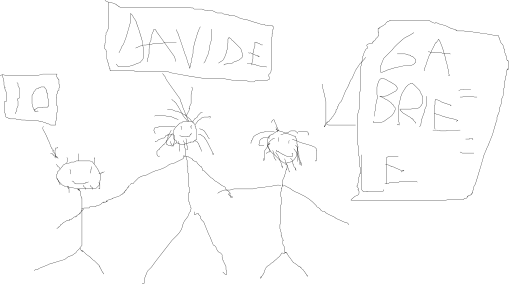
\includegraphics[width=0.7\textwidth]{gruppo_rel}
\end{center}

\vspace{ \stretch{1} }
% Le varie sezioni
%\section{Obiettivi}
\begin{abstract}
	\noindent
	L'obiettivo dell'esperienza è la misura della curva di trasferimento di un amplificatore (in configurazione invertente e non invertente) e 
lo studio della sua risposta in frequenza (in configurazione non invertente).

\end{abstract}

\newpage


\microtypesetup{protrusion=false} % disables protrusion locally in the document
\tableofcontents % prints Table of Contents
%\listoftabella
%\listoffigures
%\listoftables
\microtypesetup{protrusion=true} % enables protrusion

%\begin{multicols}{2}

% \section{Apparato strumentale}
% 	\begin{figure}
 \centering 
 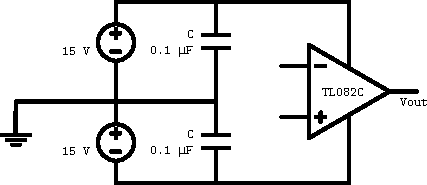
\includegraphics[width=\textwidth]{alimentazione_opamp.pdf}
 \caption{Alimentazione OpAmp} 
\end{figure}

\begin{figure}
 \centering 
 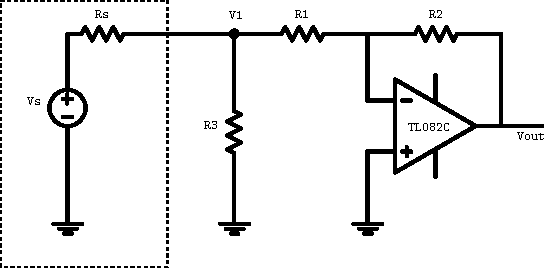
\includegraphics[width=\textwidth]{amplificazione_invertente.pdf}
 \caption{Amplificazione configurazione invertente} 
\end{figure}

\begin{figure}
 \centering 
 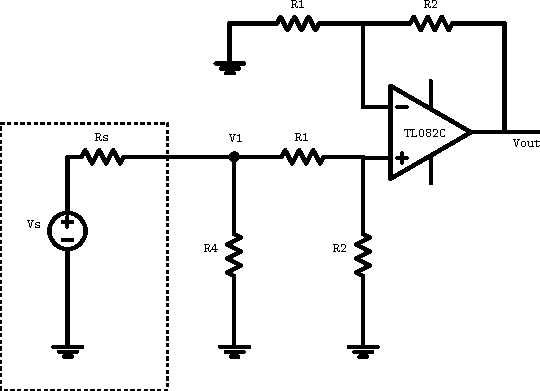
\includegraphics[width=\textwidth]{amplificazione_non_invertente.pdf}
 \caption{Amplificazione configurazione non invertente} 
\end{figure}


% \section{Metodologia di misura}
% 	\input{./sezioni/metodologia_misura.tex}

%\newpage
%\end{multicols}
% \section{Presentazione dei dati}
 	%inserire circuito
\section{Parte I}
\subsection{Amplificatore invertente}
Schema amplificatore invertente:
%inserire circuito
Le resistenze sono state scelte in modo da avere guadagno $A=-10 \frac{V}{V}$\\
$R_1=9.85 \pm 0.05\,k\Omega $\\ %mettere errore
$R_2=101.3 \pm 0.6\,k\Omega$\\ %mettere errore
$R_3=56.0 \pm 0.3\,\Omega$\\ %mettere errore

Per il calcolo degli errori sul valore delle resistenze, lette sull'Agilent U1232A, è stata utilizzata la seguente formula:
$$\sigma_{tot}=\sqrt{ \sigma^{2} _{\%} + \sigma^{2} _{dgt}}$$
Per il calcolo delle $\sigma_{tot}$ è stato cercato del datasheet dello strumento, l'errore percentuale e di digit
corrispondente al fondo scala utilizzato.

\subsubsection{Calcolo amplificazione}
Dimostrazione che amplificazione in configurazione invertente è data da %inserire dimostrazione

\subsubsection{Analisi}
La stima di A teorica, a partire dalle resistenze misurate è:
$A_{teorica}=$ %inserire valore teorico

Le misure sono state fatte applicando una tensione sinusoidale di frequenza $ f=1 \,kHz$, variando l'ampiezza tra 
$0.2 V_{pp}$ e $4 V_{pp}$.

\begin{grafico} 
 \centering 
 \begin{tikzpicture}
\pgfdeclareplotmark{cross} {
\pgfpathmoveto{\pgfpoint{-0.3\pgfplotmarksize}{\pgfplotmarksize}}
\pgfpathlineto{\pgfpoint{+0.3\pgfplotmarksize}{\pgfplotmarksize}}
\pgfpathlineto{\pgfpoint{+0.3\pgfplotmarksize}{0.3\pgfplotmarksize}}
\pgfpathlineto{\pgfpoint{+1\pgfplotmarksize}{0.3\pgfplotmarksize}}
\pgfpathlineto{\pgfpoint{+1\pgfplotmarksize}{-0.3\pgfplotmarksize}}
\pgfpathlineto{\pgfpoint{+0.3\pgfplotmarksize}{-0.3\pgfplotmarksize}}
\pgfpathlineto{\pgfpoint{+0.3\pgfplotmarksize}{-1.\pgfplotmarksize}}
\pgfpathlineto{\pgfpoint{-0.3\pgfplotmarksize}{-1.\pgfplotmarksize}}
\pgfpathlineto{\pgfpoint{-0.3\pgfplotmarksize}{-0.3\pgfplotmarksize}}
\pgfpathlineto{\pgfpoint{-1.\pgfplotmarksize}{-0.3\pgfplotmarksize}}
\pgfpathlineto{\pgfpoint{-1.\pgfplotmarksize}{0.3\pgfplotmarksize}}
\pgfpathlineto{\pgfpoint{-0.3\pgfplotmarksize}{0.3\pgfplotmarksize}}
\pgfpathclose
\pgfusepathqstroke
}
\pgfdeclareplotmark{cross*} {
\pgfpathmoveto{\pgfpoint{-0.3\pgfplotmarksize}{\pgfplotmarksize}}
\pgfpathlineto{\pgfpoint{+0.3\pgfplotmarksize}{\pgfplotmarksize}}
\pgfpathlineto{\pgfpoint{+0.3\pgfplotmarksize}{0.3\pgfplotmarksize}}
\pgfpathlineto{\pgfpoint{+1\pgfplotmarksize}{0.3\pgfplotmarksize}}
\pgfpathlineto{\pgfpoint{+1\pgfplotmarksize}{-0.3\pgfplotmarksize}}
\pgfpathlineto{\pgfpoint{+0.3\pgfplotmarksize}{-0.3\pgfplotmarksize}}
\pgfpathlineto{\pgfpoint{+0.3\pgfplotmarksize}{-1.\pgfplotmarksize}}
\pgfpathlineto{\pgfpoint{-0.3\pgfplotmarksize}{-1.\pgfplotmarksize}}
\pgfpathlineto{\pgfpoint{-0.3\pgfplotmarksize}{-0.3\pgfplotmarksize}}
\pgfpathlineto{\pgfpoint{-1.\pgfplotmarksize}{-0.3\pgfplotmarksize}}
\pgfpathlineto{\pgfpoint{-1.\pgfplotmarksize}{0.3\pgfplotmarksize}}
\pgfpathlineto{\pgfpoint{-0.3\pgfplotmarksize}{0.3\pgfplotmarksize}}
\pgfpathclose
\pgfusepathqfillstroke
}
\pgfdeclareplotmark{newstar} {
\pgfpathmoveto{\pgfqpoint{0pt}{\pgfplotmarksize}}
\pgfpathlineto{\pgfqpointpolar{44}{0.5\pgfplotmarksize}}
\pgfpathlineto{\pgfqpointpolar{18}{\pgfplotmarksize}}
\pgfpathlineto{\pgfqpointpolar{-20}{0.5\pgfplotmarksize}}
\pgfpathlineto{\pgfqpointpolar{-54}{\pgfplotmarksize}}
\pgfpathlineto{\pgfqpointpolar{-90}{0.5\pgfplotmarksize}}
\pgfpathlineto{\pgfqpointpolar{234}{\pgfplotmarksize}}
\pgfpathlineto{\pgfqpointpolar{198}{0.5\pgfplotmarksize}}
\pgfpathlineto{\pgfqpointpolar{162}{\pgfplotmarksize}}
\pgfpathlineto{\pgfqpointpolar{134}{0.5\pgfplotmarksize}}
\pgfpathclose
\pgfusepathqstroke
}
\pgfdeclareplotmark{newstar*} {
\pgfpathmoveto{\pgfqpoint{0pt}{\pgfplotmarksize}}
\pgfpathlineto{\pgfqpointpolar{44}{0.5\pgfplotmarksize}}
\pgfpathlineto{\pgfqpointpolar{18}{\pgfplotmarksize}}
\pgfpathlineto{\pgfqpointpolar{-20}{0.5\pgfplotmarksize}}
\pgfpathlineto{\pgfqpointpolar{-54}{\pgfplotmarksize}}
\pgfpathlineto{\pgfqpointpolar{-90}{0.5\pgfplotmarksize}}
\pgfpathlineto{\pgfqpointpolar{234}{\pgfplotmarksize}}
\pgfpathlineto{\pgfqpointpolar{198}{0.5\pgfplotmarksize}}
\pgfpathlineto{\pgfqpointpolar{162}{\pgfplotmarksize}}
\pgfpathlineto{\pgfqpointpolar{134}{0.5\pgfplotmarksize}}
\pgfpathclose
\pgfusepathqfillstroke
}
\definecolor{c}{rgb}{1,1,1};
\draw [color=c, fill=c] (0,0) rectangle (20,13.5632);
\definecolor{c}{rgb}{0.8,0.78,0.67};
\draw [color=c, fill=c] (2,1.35632) rectangle (18,12.2069);
\definecolor{c}{rgb}{0,0,0};
\draw [c,line width=0.9] (2,1.35632) -- (2,12.2069) -- (18,12.2069) -- (18,1.35632) -- (2,1.35632);
\definecolor{c}{rgb}{0.8,0.78,0.67};
\draw [color=c, fill=c] (2,1.35632) rectangle (18,12.2069);
\definecolor{c}{rgb}{0,0,0};
\draw [c,line width=0.9] (2,1.35632) -- (2,12.2069) -- (18,12.2069) -- (18,1.35632) -- (2,1.35632);
\draw [c,line width=0.9] (2,1.35632) -- (18,1.35632);
\draw [c,dotted,line width=0.9] (3.78447,12.2069) -- (3.78447,1.35632);
\draw [c,dotted,line width=0.9] (6.89224,12.2069) -- (6.89224,1.35632);
\draw [c,dotted,line width=0.9] (10,12.2069) -- (10,1.35632);
\draw [c,dotted,line width=0.9] (13.1078,12.2069) -- (13.1078,1.35632);
\draw [c,dotted,line width=0.9] (16.2155,12.2069) -- (16.2155,1.35632);
\draw [c,dotted,line width=0.9] (3.78447,12.2069) -- (3.78447,1.35632);
\draw [c,dotted,line width=0.9] (16.2155,12.2069) -- (16.2155,1.35632);
\draw [c,line width=0.9] (2,1.35632) -- (2,12.2069);
\draw [c,dotted,line width=0.9] (18,2.13085) -- (2,2.13085);
\draw [c,dotted,line width=0.9] (18,3.64523) -- (2,3.64523);
\draw [c,dotted,line width=0.9] (18,5.1596) -- (2,5.1596);
\draw [c,dotted,line width=0.9] (18,6.67397) -- (2,6.67397);
\draw [c,dotted,line width=0.9] (18,8.18834) -- (2,8.18834);
\draw [c,dotted,line width=0.9] (18,9.70271) -- (2,9.70271);
\draw [c,dotted,line width=0.9] (18,11.2171) -- (2,11.2171);
\draw [c,dotted,line width=0.9] (18,2.13085) -- (2,2.13085);
\draw [c,dotted,line width=0.9] (18,11.2171) -- (2,11.2171);
\draw [c,line width=0.9] (2,1.35632) -- (18,1.35632);
\draw [anchor= east] (18,0.596782) node[scale=1.08496, color=c, rotate=0]{$V_{out} [V]$};
\draw [c,line width=0.9] (3.78447,1.68184) -- (3.78447,1.35632);
\draw [c,line width=0.9] (4.40603,1.51908) -- (4.40603,1.35632);
\draw [c,line width=0.9] (5.02758,1.51908) -- (5.02758,1.35632);
\draw [c,line width=0.9] (5.64913,1.51908) -- (5.64913,1.35632);
\draw [c,line width=0.9] (6.27068,1.51908) -- (6.27068,1.35632);
\draw [c,line width=0.9] (6.89224,1.68184) -- (6.89224,1.35632);
\draw [c,line width=0.9] (7.51379,1.51908) -- (7.51379,1.35632);
\draw [c,line width=0.9] (8.13534,1.51908) -- (8.13534,1.35632);
\draw [c,line width=0.9] (8.7569,1.51908) -- (8.7569,1.35632);
\draw [c,line width=0.9] (9.37845,1.51908) -- (9.37845,1.35632);
\draw [c,line width=0.9] (10,1.68184) -- (10,1.35632);
\draw [c,line width=0.9] (10.6216,1.51908) -- (10.6216,1.35632);
\draw [c,line width=0.9] (11.2431,1.51908) -- (11.2431,1.35632);
\draw [c,line width=0.9] (11.8647,1.51908) -- (11.8647,1.35632);
\draw [c,line width=0.9] (12.4862,1.51908) -- (12.4862,1.35632);
\draw [c,line width=0.9] (13.1078,1.68184) -- (13.1078,1.35632);
\draw [c,line width=0.9] (13.7293,1.51908) -- (13.7293,1.35632);
\draw [c,line width=0.9] (14.3509,1.51908) -- (14.3509,1.35632);
\draw [c,line width=0.9] (14.9724,1.51908) -- (14.9724,1.35632);
\draw [c,line width=0.9] (15.594,1.51908) -- (15.594,1.35632);
\draw [c,line width=0.9] (16.2155,1.68184) -- (16.2155,1.35632);
\draw [c,line width=0.9] (3.78447,1.68184) -- (3.78447,1.35632);
\draw [c,line width=0.9] (3.16292,1.51908) -- (3.16292,1.35632);
\draw [c,line width=0.9] (2.54137,1.51908) -- (2.54137,1.35632);
\draw [c,line width=0.9] (16.2155,1.68184) -- (16.2155,1.35632);
\draw [c,line width=0.9] (16.8371,1.51908) -- (16.8371,1.35632);
\draw [c,line width=0.9] (17.4586,1.51908) -- (17.4586,1.35632);
\draw [anchor=base] (3.78447,0.908736) node[scale=1.08496, color=c, rotate=0]{-2};
\draw [anchor=base] (6.89224,0.908736) node[scale=1.08496, color=c, rotate=0]{-1};
\draw [anchor=base] (10,0.908736) node[scale=1.08496, color=c, rotate=0]{0};
\draw [anchor=base] (13.1078,0.908736) node[scale=1.08496, color=c, rotate=0]{1};
\draw [anchor=base] (16.2155,0.908736) node[scale=1.08496, color=c, rotate=0]{2};
\draw [c,line width=0.9] (2,1.35632) -- (2,12.2069);
\draw [anchor= east] (0.88,12.2069) node[scale=1.08496, color=c, rotate=90]{$V_{in} [V]$};
\draw [c,line width=0.9] (2.48,2.13085) -- (2,2.13085);
\draw [c,line width=0.9] (2.24,2.43373) -- (2,2.43373);
\draw [c,line width=0.9] (2.24,2.7366) -- (2,2.7366);
\draw [c,line width=0.9] (2.24,3.03948) -- (2,3.03948);
\draw [c,line width=0.9] (2.24,3.34235) -- (2,3.34235);
\draw [c,line width=0.9] (2.48,3.64523) -- (2,3.64523);
\draw [c,line width=0.9] (2.24,3.9481) -- (2,3.9481);
\draw [c,line width=0.9] (2.24,4.25097) -- (2,4.25097);
\draw [c,line width=0.9] (2.24,4.55385) -- (2,4.55385);
\draw [c,line width=0.9] (2.24,4.85672) -- (2,4.85672);
\draw [c,line width=0.9] (2.48,5.1596) -- (2,5.1596);
\draw [c,line width=0.9] (2.24,5.46247) -- (2,5.46247);
\draw [c,line width=0.9] (2.24,5.76535) -- (2,5.76535);
\draw [c,line width=0.9] (2.24,6.06822) -- (2,6.06822);
\draw [c,line width=0.9] (2.24,6.37109) -- (2,6.37109);
\draw [c,line width=0.9] (2.48,6.67397) -- (2,6.67397);
\draw [c,line width=0.9] (2.24,6.97684) -- (2,6.97684);
\draw [c,line width=0.9] (2.24,7.27972) -- (2,7.27972);
\draw [c,line width=0.9] (2.24,7.58259) -- (2,7.58259);
\draw [c,line width=0.9] (2.24,7.88546) -- (2,7.88546);
\draw [c,line width=0.9] (2.48,8.18834) -- (2,8.18834);
\draw [c,line width=0.9] (2.24,8.49121) -- (2,8.49121);
\draw [c,line width=0.9] (2.24,8.79409) -- (2,8.79409);
\draw [c,line width=0.9] (2.24,9.09696) -- (2,9.09696);
\draw [c,line width=0.9] (2.24,9.39984) -- (2,9.39984);
\draw [c,line width=0.9] (2.48,9.70271) -- (2,9.70271);
\draw [c,line width=0.9] (2.24,10.0056) -- (2,10.0056);
\draw [c,line width=0.9] (2.24,10.3085) -- (2,10.3085);
\draw [c,line width=0.9] (2.24,10.6113) -- (2,10.6113);
\draw [c,line width=0.9] (2.24,10.9142) -- (2,10.9142);
\draw [c,line width=0.9] (2.48,11.2171) -- (2,11.2171);
\draw [c,line width=0.9] (2.48,2.13085) -- (2,2.13085);
\draw [c,line width=0.9] (2.24,1.82798) -- (2,1.82798);
\draw [c,line width=0.9] (2.24,1.52511) -- (2,1.52511);
\draw [c,line width=0.9] (2.48,11.2171) -- (2,11.2171);
\draw [c,line width=0.9] (2.24,11.52) -- (2,11.52);
\draw [c,line width=0.9] (2.24,11.8228) -- (2,11.8228);
\draw [c,line width=0.9] (2.24,12.1257) -- (2,12.1257);
\draw [anchor= east] (1.9,2.13085) node[scale=1.08496, color=c, rotate=0]{-15};
\draw [anchor= east] (1.9,3.64523) node[scale=1.08496, color=c, rotate=0]{-10};
\draw [anchor= east] (1.9,5.1596) node[scale=1.08496, color=c, rotate=0]{-5};
\draw [anchor= east] (1.9,6.67397) node[scale=1.08496, color=c, rotate=0]{0};
\draw [anchor= east] (1.9,8.18834) node[scale=1.08496, color=c, rotate=0]{5};
\draw [anchor= east] (1.9,9.70271) node[scale=1.08496, color=c, rotate=0]{10};
\draw [anchor= east] (1.9,11.2171) node[scale=1.08496, color=c, rotate=0]{15};
\definecolor{c}{rgb}{0,0,1};
\foreach \P in {(13.2942,3.43321), (6.76793,9.88443), (10.3325,6.35898), (9.66436,7.00107), (11.3426,5.39584), (8.68852,7.98238), (12.2625,4.46904), (7.71269,8.92735), (14.2266,2.4943), (5.71129,10.8839), (15.221,2.40344), (4.77896,11.1868),
 (16.1844,2.37315), (3.81555,11.1868), (16.4952,2.37315), (3.50478,11.1868)}{\draw[mark options={color=c,fill=c},mark size=1.681682pt,mark=*,mark size=1pt] plot coordinates {\P};}
\definecolor{c}{rgb}{0,1,0};
\draw [c,line width=0.9] (5.38497,11.1925) -- (5.4782,11.1013) -- (5.57144,11.0102) -- (5.66467,10.919) -- (5.7579,10.8279) -- (5.85114,10.7367) -- (5.94437,10.6456) -- (6.0376,10.5544) -- (6.13084,10.4632) -- (6.22407,10.3721) -- (6.3173,10.2809) --
 (6.41053,10.1898) -- (6.50377,10.0986) -- (6.597,10.0075) -- (6.69023,9.91629) -- (6.78346,9.82514) -- (6.8767,9.73398) -- (6.96993,9.64282) -- (7.06316,9.55166) -- (7.1564,9.4605) -- (7.24963,9.36935) -- (7.34286,9.27819) -- (7.4361,9.18703) --
 (7.52933,9.09587) -- (7.62256,9.00471) -- (7.71579,8.91356) -- (7.80903,8.8224) -- (7.90226,8.73124) -- (7.99549,8.64008) -- (8.08873,8.54892) -- (8.18196,8.45777) -- (8.27519,8.36661) -- (8.36842,8.27545) -- (8.46166,8.18429) -- (8.55489,8.09313)
 -- (8.64812,8.00198) -- (8.74136,7.91082) -- (8.83459,7.81966) -- (8.92782,7.7285) -- (9.02105,7.63734) -- (9.11429,7.54618) -- (9.20752,7.45503) -- (9.30075,7.36387) -- (9.39399,7.27271) -- (9.48722,7.18155) -- (9.58045,7.09039) --
 (9.67369,6.99924) -- (9.76692,6.90808) -- (9.86015,6.81692) -- (9.95338,6.72576);
\draw [c,line width=0.9] (9.95338,6.72576) -- (10.0466,6.6346) -- (10.1398,6.54345) -- (10.2331,6.45229) -- (10.3263,6.36113) -- (10.4195,6.26997) -- (10.5128,6.17881) -- (10.606,6.08766) -- (10.6992,5.9965) -- (10.7925,5.90534) -- (10.8857,5.81418)
 -- (10.9789,5.72302) -- (11.0722,5.63187) -- (11.1654,5.54071) -- (11.2586,5.44955) -- (11.3519,5.35839) -- (11.4451,5.26723) -- (11.5383,5.17607) -- (11.6316,5.08492) -- (11.7248,4.99376) -- (11.818,4.9026) -- (11.9113,4.81144) -- (12.0045,4.72028)
 -- (12.0977,4.62913) -- (12.191,4.53797) -- (12.2842,4.44681) -- (12.3774,4.35565) -- (12.4707,4.26449) -- (12.5639,4.17334) -- (12.6571,4.08218) -- (12.7504,3.99102) -- (12.8436,3.89986) -- (12.9368,3.8087) -- (13.0301,3.71755) -- (13.1233,3.62639)
 -- (13.2165,3.53523) -- (13.3098,3.44407) -- (13.403,3.35291) -- (13.4962,3.26176) -- (13.5895,3.1706) -- (13.6827,3.07944) -- (13.7759,2.98828) -- (13.8692,2.89712) -- (13.9624,2.80597) -- (14.0556,2.71481) -- (14.1489,2.62365) -- (14.2421,2.53249)
 -- (14.3353,2.44133) -- (14.4286,2.35017) -- (14.5218,2.25902);
\draw [c,line width=0.9] (14.5218,2.25902) -- (14.615,2.16786);
\definecolor{c}{rgb}{1,0,0};
\draw [c,line width=0.9] (13.2942,3.43321) -- (13.2078,3.43321);
\draw [c,line width=0.9] (13.2078,3.37574) -- (13.2078,3.49068);
\draw [c,line width=0.9] (13.2942,3.43321) -- (13.3807,3.43321);
\draw [c,line width=0.9] (13.3807,3.37574) -- (13.3807,3.49068);
\draw [c,line width=0.9] (13.2942,3.43321) -- (13.2942,3.51791);
\draw [c,line width=0.9] (13.2368,3.51791) -- (13.3517,3.51791);
\draw [c,line width=0.9] (13.2942,3.43321) -- (13.2942,3.34852);
\draw [c,line width=0.9] (13.2368,3.34852) -- (13.3517,3.34852);
\draw [c,line width=0.9] (6.76793,9.88443) -- (6.68244,9.88443);
\draw [c,line width=0.9] (6.68244,9.82696) -- (6.68244,9.94191);
\draw [c,line width=0.9] (6.76793,9.88443) -- (6.85341,9.88443);
\draw [c,line width=0.9] (6.85341,9.82696) -- (6.85341,9.94191);
\draw [c,line width=0.9] (6.76793,9.88443) -- (6.76793,9.96867);
\draw [c,line width=0.9] (6.71045,9.96867) -- (6.8254,9.96867);
\draw [c,line width=0.9] (6.76793,9.88443) -- (6.76793,9.8002);
\draw [c,line width=0.9] (6.71045,9.8002) -- (6.8254,9.8002);
\draw [c,line width=0.9] (10.3325,6.35898) -- (10.3238,6.35898);
\draw [c,line width=0.9] (10.3238,6.30151) -- (10.3238,6.41645);
\draw [c,line width=0.9] (10.3325,6.35898) -- (10.3412,6.35898);
\draw [c,line width=0.9] (10.3412,6.30151) -- (10.3412,6.41645);
\draw [c,line width=0.9] (10.3325,6.35898) -- (10.3325,6.36731);
\draw [c,line width=0.9] (10.2751,6.36731) -- (10.39,6.36731);
\draw [c,line width=0.9] (10.3325,6.35898) -- (10.3325,6.35065);
\draw [c,line width=0.9] (10.2751,6.35065) -- (10.39,6.35065);
\draw [c,line width=0.9] (9.66436,7.00107) -- (9.65562,7.00107);
\draw [c,line width=0.9] (9.65562,6.9436) -- (9.65562,7.05854);
\draw [c,line width=0.9] (9.66436,7.00107) -- (9.6731,7.00107);
\draw [c,line width=0.9] (9.6731,6.9436) -- (9.6731,7.05854);
\draw [c,line width=0.9] (9.66436,7.00107) -- (9.66436,7.00959);
\draw [c,line width=0.9] (9.60689,7.00959) -- (9.72183,7.00959);
\draw [c,line width=0.9] (9.66436,7.00107) -- (9.66436,6.99256);
\draw [c,line width=0.9] (9.60689,6.99256) -- (9.72183,6.99256);
\draw [c,line width=0.9] (11.3426,5.39584) -- (11.3076,5.39584);
\draw [c,line width=0.9] (11.3076,5.33837) -- (11.3076,5.45331);
\draw [c,line width=0.9] (11.3426,5.39584) -- (11.3775,5.39584);
\draw [c,line width=0.9] (11.3775,5.33837) -- (11.3775,5.45331);
\draw [c,line width=0.9] (11.3426,5.39584) -- (11.3426,5.42944);
\draw [c,line width=0.9] (11.2851,5.42944) -- (11.4,5.42944);
\draw [c,line width=0.9] (11.3426,5.39584) -- (11.3426,5.36224);
\draw [c,line width=0.9] (11.2851,5.36224) -- (11.4,5.36224);
\draw [c,line width=0.9] (8.68852,7.98238) -- (8.65405,7.98238);
\draw [c,line width=0.9] (8.65405,7.92491) -- (8.65405,8.03986);
\draw [c,line width=0.9] (8.68852,7.98238) -- (8.723,7.98238);
\draw [c,line width=0.9] (8.723,7.92491) -- (8.723,8.03986);
\draw [c,line width=0.9] (8.68852,7.98238) -- (8.68852,8.01645);
\draw [c,line width=0.9] (8.63105,8.01645) -- (8.746,8.01645);
\draw [c,line width=0.9] (8.68852,7.98238) -- (8.68852,7.94832);
\draw [c,line width=0.9] (8.63105,7.94832) -- (8.746,7.94832);
\draw [c,line width=0.9] (12.2625,4.46904) -- (12.2038,4.46904);
\draw [c,line width=0.9] (12.2038,4.41157) -- (12.2038,4.52651);
\draw [c,line width=0.9] (12.2625,4.46904) -- (12.3211,4.46904);
\draw [c,line width=0.9] (12.3211,4.41157) -- (12.3211,4.52651);
\draw [c,line width=0.9] (12.2625,4.46904) -- (12.2625,4.52619);
\draw [c,line width=0.9] (12.205,4.52619) -- (12.3199,4.52619);
\draw [c,line width=0.9] (12.2625,4.46904) -- (12.2625,4.4119);
\draw [c,line width=0.9] (12.205,4.4119) -- (12.3199,4.4119);
\draw [c,line width=0.9] (7.71269,8.92735) -- (7.65367,8.92735);
\draw [c,line width=0.9] (7.65367,8.86988) -- (7.65367,8.98482);
\draw [c,line width=0.9] (7.71269,8.92735) -- (7.77171,8.92735);
\draw [c,line width=0.9] (7.77171,8.86988) -- (7.77171,8.98482);
\draw [c,line width=0.9] (7.71269,8.92735) -- (7.71269,8.98525);
\draw [c,line width=0.9] (7.65522,8.98525) -- (7.77016,8.98525);
\draw [c,line width=0.9] (7.71269,8.92735) -- (7.71269,8.86946);
\draw [c,line width=0.9] (7.65522,8.86946) -- (7.77016,8.86946);
\draw [c,line width=0.9] (14.2266,2.4943) -- (14.1138,2.4943);
\draw [c,line width=0.9] (14.1138,2.43683) -- (14.1138,2.55177);
\draw [c,line width=0.9] (14.2266,2.4943) -- (14.3393,2.4943);
\draw [c,line width=0.9] (14.3393,2.43683) -- (14.3393,2.55177);
\draw [c,line width=0.9] (14.2266,2.4943) -- (14.2266,2.60508);
\draw [c,line width=0.9] (14.1691,2.60508) -- (14.284,2.60508);
\draw [c,line width=0.9] (14.2266,2.4943) -- (14.2266,2.38353);
\draw [c,line width=0.9] (14.1691,2.38353) -- (14.284,2.38353);
\draw [c,line width=0.9] (5.71129,10.8839) -- (5.59762,10.8839);
\draw [c,line width=0.9] (5.59762,10.8264) -- (5.59762,10.9414);
\draw [c,line width=0.9] (5.71129,10.8839) -- (5.82495,10.8839);
\draw [c,line width=0.9] (5.82495,10.8264) -- (5.82495,10.9414);
\draw [c,line width=0.9] (5.71129,10.8839) -- (5.71129,10.9952);
\draw [c,line width=0.9] (5.65382,10.9952) -- (5.76876,10.9952);
\draw [c,line width=0.9] (5.71129,10.8839) -- (5.71129,10.7727);
\draw [c,line width=0.9] (5.65382,10.7727) -- (5.76876,10.7727);
\draw [c,line width=0.9] (15.221,2.40344) -- (15.0811,2.40344);
\draw [c,line width=0.9] (15.0811,2.34597) -- (15.0811,2.46091);
\draw [c,line width=0.9] (15.221,2.40344) -- (15.361,2.40344);
\draw [c,line width=0.9] (15.361,2.34597) -- (15.361,2.46091);
\draw [c,line width=0.9] (15.221,2.40344) -- (15.221,2.5156);
\draw [c,line width=0.9] (15.1636,2.5156) -- (15.2785,2.5156);
\draw [c,line width=0.9] (15.221,2.40344) -- (15.221,2.29129);
\draw [c,line width=0.9] (15.1636,2.29129) -- (15.2785,2.29129);
\draw [c,line width=0.9] (4.77896,11.1868) -- (4.63897,11.1868);
\draw [c,line width=0.9] (4.63897,11.1293) -- (4.63897,11.2443);
\draw [c,line width=0.9] (4.77896,11.1868) -- (4.91894,11.1868);
\draw [c,line width=0.9] (4.91894,11.1293) -- (4.91894,11.2443);
\draw [c,line width=0.9] (4.77896,11.1868) -- (4.77896,11.3027);
\draw [c,line width=0.9] (4.72149,11.3027) -- (4.83643,11.3027);
\draw [c,line width=0.9] (4.77896,11.1868) -- (4.77896,11.0709);
\draw [c,line width=0.9] (4.72149,11.0709) -- (4.83643,11.0709);
\draw [c,line width=0.9] (16.1844,2.37315) -- (16.0177,2.37315);
\draw [c,line width=0.9] (16.0177,2.31568) -- (16.0177,2.43062);
\draw [c,line width=0.9] (16.1844,2.37315) -- (16.3512,2.37315);
\draw [c,line width=0.9] (16.3512,2.31568) -- (16.3512,2.43062);
\draw [c,line width=0.9] (16.1844,2.37315) -- (16.1844,2.48577);
\draw [c,line width=0.9] (16.127,2.48577) -- (16.2419,2.48577);
\draw [c,line width=0.9] (16.1844,2.37315) -- (16.1844,2.26054);
\draw [c,line width=0.9] (16.127,2.26054) -- (16.2419,2.26054);
\draw [c,line width=0.9] (3.81555,11.1868) -- (3.64877,11.1868);
\draw [c,line width=0.9] (3.64877,11.1293) -- (3.64877,11.2443);
\draw [c,line width=0.9] (3.81555,11.1868) -- (3.98233,11.1868);
\draw [c,line width=0.9] (3.98233,11.1293) -- (3.98233,11.2443);
\draw [c,line width=0.9] (3.81555,11.1868) -- (3.81555,11.3027);
\draw [c,line width=0.9] (3.75808,11.3027) -- (3.87302,11.3027);
\draw [c,line width=0.9] (3.81555,11.1868) -- (3.81555,11.0709);
\draw [c,line width=0.9] (3.75808,11.0709) -- (3.87302,11.0709);
\draw [c,line width=0.9] (16.4952,2.37315) -- (16.3238,2.37315);
\draw [c,line width=0.9] (16.3238,2.31568) -- (16.3238,2.43062);
\draw [c,line width=0.9] (16.4952,2.37315) -- (16.6667,2.37315);
\draw [c,line width=0.9] (16.6667,2.31568) -- (16.6667,2.43062);
\draw [c,line width=0.9] (16.4952,2.37315) -- (16.4952,2.48577);
\draw [c,line width=0.9] (16.4378,2.48577) -- (16.5527,2.48577);
\draw [c,line width=0.9] (16.4952,2.37315) -- (16.4952,2.26054);
\draw [c,line width=0.9] (16.4378,2.26054) -- (16.5527,2.26054);
\draw [c,line width=0.9] (3.50478,11.1868) -- (3.33333,11.1868);
\draw [c,line width=0.9] (3.33333,11.1293) -- (3.33333,11.2443);
\draw [c,line width=0.9] (3.50478,11.1868) -- (3.67622,11.1868);
\draw [c,line width=0.9] (3.67622,11.1293) -- (3.67622,11.2443);
\draw [c,line width=0.9] (3.50478,11.1868) -- (3.50478,11.3027);
\draw [c,line width=0.9] (3.4473,11.3027) -- (3.56225,11.3027);
\draw [c,line width=0.9] (3.50478,11.1868) -- (3.50478,11.0709);
\draw [c,line width=0.9] (3.4473,11.0709) -- (3.56225,11.0709);
\definecolor{c}{rgb}{0,0,0};
\draw (10,13.1224) node[scale=1.40406, color=c, rotate=0]{Gain};
\end{tikzpicture}
 
 \caption{Curva di trasferimento di un amplificatore invertente} 
 \label{gr:amp_inv.tex} 
\end{grafico}

\begin{tabella}
 \centering
 \begin{center}
\begin{tabulary}{\textwidth}{CCCCCC}
\toprule
$V_{in+}$ (V) & $V_{in-}$ (V) & FS (V) & $V_{out+}$(V) & $V_{out-}$ (V) & FS (V) \\ \midrule 
1.06 & -1.04 & 0.3 & -10.7 & 10.6 & 3 \\ \midrule
0.107 & -0.108 & 0.03 & -1.04 & 1.08 & 0.3 \\ \midrule
0.432 & -0.422 & 0.12 & -4.22 & 4.32 & 1.2 \\ \midrule
0.728 & -0.736 & 0.2 & -7.28 & 7.44 & 2 \\ \midrule
1.36 & -1.38 & 0.4 & -13.8 & 13.9 & 4 \\ \midrule
1.68 & -1.68 & 0.5 & -14.1 & 14.9 & 4 \\ \midrule
1.99 & -1.99 & 0.6 & -14.2 & 14.9 & 4 \\ \midrule
2.09 & -2.09 & 0.6 & -14.2 & 14.9 & 4 \\ \midrule

 \bottomrule
\end{tabulary}
\end{center}
 
 \caption{Dati curva di trasferimento}
 \label{tab:tab_inv.tex}
\end{tabella}

Per il calcolo degli errori sui valori di $V_{in}$ e $V_{out}$ letti sull'oscilloscopio, è stata utilizzata la seguente formula:
$$\sigma_{tot}=\sqrt{ (0.02\cdot V_{letto})^2 + (0.06 \cdot V_{div})^2}$$

E' stata fatta l'interpolazione lineare pesata dei punti compresi tra 0 e 1.5 V.\\
$q = 0.02 \pm 0.03 \,V$\\
$m = -10.0 \pm 0.1 \, \frac{V}{V}$




\subsection{Amplificatore non invertente}

Schema amplificatore non invertente:
%inserire circuito
Le resistenze sono state scelte in modo da avere guadagno $A=10 \frac{V}{V}$\\
$R_{1,up}=9.91 \pm0.05 \,k\Omega $\\ %mettere errore
$R_{1,down}=9.85 \pm 0.05\,k\Omega$\\ %mettere errore
$R_{2,up}=99.7 \pm 0.6\,k\Omega$\\ %mettere errore
$R_{2,down}=101.3 \pm 0.6\,k\Omega$\\
$R_4=56.0 \pm 0.3\,\Omega$

\subsubsection{Calcolo amplificazione}
Dimostrazione che amplificazione in configurazione non invertente è data da %inserire dimostrazione

\subsubsection{Analisi}
La stima di A teorica, a partire dalle resistenze misurate è:\\
$A_{teorica}=$ %inserire valore teorico

Le misure sono state fatte applicando una tensione sinusoidale di frequenza $ f=1 \,kHz$, variando l'ampiezza tra 
$0.2 V_{pp}$ e $4 V_{pp}$.

\begin{grafico} 
 \centering 
 \begin{tikzpicture}
\pgfdeclareplotmark{cross} {
\pgfpathmoveto{\pgfpoint{-0.3\pgfplotmarksize}{\pgfplotmarksize}}
\pgfpathlineto{\pgfpoint{+0.3\pgfplotmarksize}{\pgfplotmarksize}}
\pgfpathlineto{\pgfpoint{+0.3\pgfplotmarksize}{0.3\pgfplotmarksize}}
\pgfpathlineto{\pgfpoint{+1\pgfplotmarksize}{0.3\pgfplotmarksize}}
\pgfpathlineto{\pgfpoint{+1\pgfplotmarksize}{-0.3\pgfplotmarksize}}
\pgfpathlineto{\pgfpoint{+0.3\pgfplotmarksize}{-0.3\pgfplotmarksize}}
\pgfpathlineto{\pgfpoint{+0.3\pgfplotmarksize}{-1.\pgfplotmarksize}}
\pgfpathlineto{\pgfpoint{-0.3\pgfplotmarksize}{-1.\pgfplotmarksize}}
\pgfpathlineto{\pgfpoint{-0.3\pgfplotmarksize}{-0.3\pgfplotmarksize}}
\pgfpathlineto{\pgfpoint{-1.\pgfplotmarksize}{-0.3\pgfplotmarksize}}
\pgfpathlineto{\pgfpoint{-1.\pgfplotmarksize}{0.3\pgfplotmarksize}}
\pgfpathlineto{\pgfpoint{-0.3\pgfplotmarksize}{0.3\pgfplotmarksize}}
\pgfpathclose
\pgfusepathqstroke
}
\pgfdeclareplotmark{cross*} {
\pgfpathmoveto{\pgfpoint{-0.3\pgfplotmarksize}{\pgfplotmarksize}}
\pgfpathlineto{\pgfpoint{+0.3\pgfplotmarksize}{\pgfplotmarksize}}
\pgfpathlineto{\pgfpoint{+0.3\pgfplotmarksize}{0.3\pgfplotmarksize}}
\pgfpathlineto{\pgfpoint{+1\pgfplotmarksize}{0.3\pgfplotmarksize}}
\pgfpathlineto{\pgfpoint{+1\pgfplotmarksize}{-0.3\pgfplotmarksize}}
\pgfpathlineto{\pgfpoint{+0.3\pgfplotmarksize}{-0.3\pgfplotmarksize}}
\pgfpathlineto{\pgfpoint{+0.3\pgfplotmarksize}{-1.\pgfplotmarksize}}
\pgfpathlineto{\pgfpoint{-0.3\pgfplotmarksize}{-1.\pgfplotmarksize}}
\pgfpathlineto{\pgfpoint{-0.3\pgfplotmarksize}{-0.3\pgfplotmarksize}}
\pgfpathlineto{\pgfpoint{-1.\pgfplotmarksize}{-0.3\pgfplotmarksize}}
\pgfpathlineto{\pgfpoint{-1.\pgfplotmarksize}{0.3\pgfplotmarksize}}
\pgfpathlineto{\pgfpoint{-0.3\pgfplotmarksize}{0.3\pgfplotmarksize}}
\pgfpathclose
\pgfusepathqfillstroke
}
\pgfdeclareplotmark{newstar} {
\pgfpathmoveto{\pgfqpoint{0pt}{\pgfplotmarksize}}
\pgfpathlineto{\pgfqpointpolar{44}{0.5\pgfplotmarksize}}
\pgfpathlineto{\pgfqpointpolar{18}{\pgfplotmarksize}}
\pgfpathlineto{\pgfqpointpolar{-20}{0.5\pgfplotmarksize}}
\pgfpathlineto{\pgfqpointpolar{-54}{\pgfplotmarksize}}
\pgfpathlineto{\pgfqpointpolar{-90}{0.5\pgfplotmarksize}}
\pgfpathlineto{\pgfqpointpolar{234}{\pgfplotmarksize}}
\pgfpathlineto{\pgfqpointpolar{198}{0.5\pgfplotmarksize}}
\pgfpathlineto{\pgfqpointpolar{162}{\pgfplotmarksize}}
\pgfpathlineto{\pgfqpointpolar{134}{0.5\pgfplotmarksize}}
\pgfpathclose
\pgfusepathqstroke
}
\pgfdeclareplotmark{newstar*} {
\pgfpathmoveto{\pgfqpoint{0pt}{\pgfplotmarksize}}
\pgfpathlineto{\pgfqpointpolar{44}{0.5\pgfplotmarksize}}
\pgfpathlineto{\pgfqpointpolar{18}{\pgfplotmarksize}}
\pgfpathlineto{\pgfqpointpolar{-20}{0.5\pgfplotmarksize}}
\pgfpathlineto{\pgfqpointpolar{-54}{\pgfplotmarksize}}
\pgfpathlineto{\pgfqpointpolar{-90}{0.5\pgfplotmarksize}}
\pgfpathlineto{\pgfqpointpolar{234}{\pgfplotmarksize}}
\pgfpathlineto{\pgfqpointpolar{198}{0.5\pgfplotmarksize}}
\pgfpathlineto{\pgfqpointpolar{162}{\pgfplotmarksize}}
\pgfpathlineto{\pgfqpointpolar{134}{0.5\pgfplotmarksize}}
\pgfpathclose
\pgfusepathqfillstroke
}
\definecolor{c}{rgb}{1,1,1};
\draw [color=c, fill=c] (0,0) rectangle (20,13.5632);
\definecolor{c}{rgb}{0.8,0.78,0.67};
\draw [color=c, fill=c] (2,1.35632) rectangle (18,12.2069);
\definecolor{c}{rgb}{0,0,0};
\draw [c,line width=0.9] (2,1.35632) -- (2,12.2069) -- (18,12.2069) -- (18,1.35632) -- (2,1.35632);
\definecolor{c}{rgb}{0.8,0.78,0.67};
\draw [color=c, fill=c] (2,1.35632) rectangle (18,12.2069);
\definecolor{c}{rgb}{0,0,0};
\draw [c,line width=0.9] (2,1.35632) -- (2,12.2069) -- (18,12.2069) -- (18,1.35632) -- (2,1.35632);
\draw [c,line width=0.9] (2,1.35632) -- (18,1.35632);
\draw [c,dotted,line width=0.9] (3.7792,12.2069) -- (3.7792,1.35632);
\draw [c,dotted,line width=0.9] (6.85062,12.2069) -- (6.85062,1.35632);
\draw [c,dotted,line width=0.9] (9.92204,12.2069) -- (9.92204,1.35632);
\draw [c,dotted,line width=0.9] (12.9935,12.2069) -- (12.9935,1.35632);
\draw [c,dotted,line width=0.9] (16.0649,12.2069) -- (16.0649,1.35632);
\draw [c,dotted,line width=0.9] (3.7792,12.2069) -- (3.7792,1.35632);
\draw [c,dotted,line width=0.9] (16.0649,12.2069) -- (16.0649,1.35632);
\draw [c,line width=0.9] (2,1.35632) -- (2,12.2069);
\draw [c,dotted,line width=0.9] (18,2.19282) -- (2,2.19282);
\draw [c,dotted,line width=0.9] (18,3.69696) -- (2,3.69696);
\draw [c,dotted,line width=0.9] (18,5.2011) -- (2,5.2011);
\draw [c,dotted,line width=0.9] (18,6.70524) -- (2,6.70524);
\draw [c,dotted,line width=0.9] (18,8.20938) -- (2,8.20938);
\draw [c,dotted,line width=0.9] (18,9.71352) -- (2,9.71352);
\draw [c,dotted,line width=0.9] (18,11.2177) -- (2,11.2177);
\draw [c,dotted,line width=0.9] (18,2.19282) -- (2,2.19282);
\draw [c,dotted,line width=0.9] (18,11.2177) -- (2,11.2177);
\draw [c,line width=0.9] (2,1.35632) -- (18,1.35632);
\draw [anchor= east] (18,0.596782) node[scale=1.08496, color=c, rotate=0]{$V_{out} [V]$};
\draw [c,line width=0.9] (3.7792,1.68184) -- (3.7792,1.35632);
\draw [c,line width=0.9] (4.39348,1.51908) -- (4.39348,1.35632);
\draw [c,line width=0.9] (5.00777,1.51908) -- (5.00777,1.35632);
\draw [c,line width=0.9] (5.62205,1.51908) -- (5.62205,1.35632);
\draw [c,line width=0.9] (6.23634,1.51908) -- (6.23634,1.35632);
\draw [c,line width=0.9] (6.85062,1.68184) -- (6.85062,1.35632);
\draw [c,line width=0.9] (7.46491,1.51908) -- (7.46491,1.35632);
\draw [c,line width=0.9] (8.07919,1.51908) -- (8.07919,1.35632);
\draw [c,line width=0.9] (8.69348,1.51908) -- (8.69348,1.35632);
\draw [c,line width=0.9] (9.30776,1.51908) -- (9.30776,1.35632);
\draw [c,line width=0.9] (9.92204,1.68184) -- (9.92204,1.35632);
\draw [c,line width=0.9] (10.5363,1.51908) -- (10.5363,1.35632);
\draw [c,line width=0.9] (11.1506,1.51908) -- (11.1506,1.35632);
\draw [c,line width=0.9] (11.7649,1.51908) -- (11.7649,1.35632);
\draw [c,line width=0.9] (12.3792,1.51908) -- (12.3792,1.35632);
\draw [c,line width=0.9] (12.9935,1.68184) -- (12.9935,1.35632);
\draw [c,line width=0.9] (13.6078,1.51908) -- (13.6078,1.35632);
\draw [c,line width=0.9] (14.222,1.51908) -- (14.222,1.35632);
\draw [c,line width=0.9] (14.8363,1.51908) -- (14.8363,1.35632);
\draw [c,line width=0.9] (15.4506,1.51908) -- (15.4506,1.35632);
\draw [c,line width=0.9] (16.0649,1.68184) -- (16.0649,1.35632);
\draw [c,line width=0.9] (3.7792,1.68184) -- (3.7792,1.35632);
\draw [c,line width=0.9] (3.16491,1.51908) -- (3.16491,1.35632);
\draw [c,line width=0.9] (2.55063,1.51908) -- (2.55063,1.35632);
\draw [c,line width=0.9] (16.0649,1.68184) -- (16.0649,1.35632);
\draw [c,line width=0.9] (16.6792,1.51908) -- (16.6792,1.35632);
\draw [c,line width=0.9] (17.2935,1.51908) -- (17.2935,1.35632);
\draw [c,line width=0.9] (17.9077,1.51908) -- (17.9077,1.35632);
\draw [anchor=base] (3.7792,0.908736) node[scale=1.08496, color=c, rotate=0]{-2};
\draw [anchor=base] (6.85062,0.908736) node[scale=1.08496, color=c, rotate=0]{-1};
\draw [anchor=base] (9.92204,0.908736) node[scale=1.08496, color=c, rotate=0]{0};
\draw [anchor=base] (12.9935,0.908736) node[scale=1.08496, color=c, rotate=0]{1};
\draw [anchor=base] (16.0649,0.908736) node[scale=1.08496, color=c, rotate=0]{2};
\draw [c,line width=0.9] (2,1.35632) -- (2,12.2069);
\draw [anchor= east] (0.88,12.2069) node[scale=1.08496, color=c, rotate=90]{$V_{in} [V]$};
\draw [c,line width=0.9] (2.48,2.19282) -- (2,2.19282);
\draw [c,line width=0.9] (2.24,2.49365) -- (2,2.49365);
\draw [c,line width=0.9] (2.24,2.79447) -- (2,2.79447);
\draw [c,line width=0.9] (2.24,3.0953) -- (2,3.0953);
\draw [c,line width=0.9] (2.24,3.39613) -- (2,3.39613);
\draw [c,line width=0.9] (2.48,3.69696) -- (2,3.69696);
\draw [c,line width=0.9] (2.24,3.99779) -- (2,3.99779);
\draw [c,line width=0.9] (2.24,4.29861) -- (2,4.29861);
\draw [c,line width=0.9] (2.24,4.59944) -- (2,4.59944);
\draw [c,line width=0.9] (2.24,4.90027) -- (2,4.90027);
\draw [c,line width=0.9] (2.48,5.2011) -- (2,5.2011);
\draw [c,line width=0.9] (2.24,5.50193) -- (2,5.50193);
\draw [c,line width=0.9] (2.24,5.80275) -- (2,5.80275);
\draw [c,line width=0.9] (2.24,6.10358) -- (2,6.10358);
\draw [c,line width=0.9] (2.24,6.40441) -- (2,6.40441);
\draw [c,line width=0.9] (2.48,6.70524) -- (2,6.70524);
\draw [c,line width=0.9] (2.24,7.00607) -- (2,7.00607);
\draw [c,line width=0.9] (2.24,7.30689) -- (2,7.30689);
\draw [c,line width=0.9] (2.24,7.60772) -- (2,7.60772);
\draw [c,line width=0.9] (2.24,7.90855) -- (2,7.90855);
\draw [c,line width=0.9] (2.48,8.20938) -- (2,8.20938);
\draw [c,line width=0.9] (2.24,8.51021) -- (2,8.51021);
\draw [c,line width=0.9] (2.24,8.81104) -- (2,8.81104);
\draw [c,line width=0.9] (2.24,9.11186) -- (2,9.11186);
\draw [c,line width=0.9] (2.24,9.41269) -- (2,9.41269);
\draw [c,line width=0.9] (2.48,9.71352) -- (2,9.71352);
\draw [c,line width=0.9] (2.24,10.0143) -- (2,10.0143);
\draw [c,line width=0.9] (2.24,10.3152) -- (2,10.3152);
\draw [c,line width=0.9] (2.24,10.616) -- (2,10.616);
\draw [c,line width=0.9] (2.24,10.9168) -- (2,10.9168);
\draw [c,line width=0.9] (2.48,11.2177) -- (2,11.2177);
\draw [c,line width=0.9] (2.48,2.19282) -- (2,2.19282);
\draw [c,line width=0.9] (2.24,1.89199) -- (2,1.89199);
\draw [c,line width=0.9] (2.24,1.59116) -- (2,1.59116);
\draw [c,line width=0.9] (2.48,11.2177) -- (2,11.2177);
\draw [c,line width=0.9] (2.24,11.5185) -- (2,11.5185);
\draw [c,line width=0.9] (2.24,11.8193) -- (2,11.8193);
\draw [c,line width=0.9] (2.24,12.1201) -- (2,12.1201);
\draw [anchor= east] (1.9,2.19282) node[scale=1.08496, color=c, rotate=0]{-15};
\draw [anchor= east] (1.9,3.69696) node[scale=1.08496, color=c, rotate=0]{-10};
\draw [anchor= east] (1.9,5.2011) node[scale=1.08496, color=c, rotate=0]{-5};
\draw [anchor= east] (1.9,6.70524) node[scale=1.08496, color=c, rotate=0]{0};
\draw [anchor= east] (1.9,8.20938) node[scale=1.08496, color=c, rotate=0]{5};
\draw [anchor= east] (1.9,9.71352) node[scale=1.08496, color=c, rotate=0]{10};
\draw [anchor= east] (1.9,11.2177) node[scale=1.08496, color=c, rotate=0]{15};
\definecolor{c}{rgb}{0,0,1};
\foreach \P in {(13.2392,9.9241), (6.72776,3.48638), (10.2538,7.02712), (9.5934,6.38335), (11.2489,8.00482), (8.61055,5.4207), (12.2072,8.9434), (7.63691,4.46708), (14.1913,10.8867), (5.68348,2.52373), (15.2049,11.1876), (4.70063,2.37331),
 (16.1877,11.1274), (3.80991,2.43348), (16.4949,11.1876), (3.50277,2.43348)}{\draw[mark options={color=c,fill=c},mark size=1.681682pt,mark=*,mark size=1pt] plot coordinates {\P};}
\definecolor{c}{rgb}{0,1,0};
\draw [c,line width=0.9] (5.36098,2.22861) -- (5.45312,2.319) -- (5.54527,2.4094) -- (5.63741,2.4998) -- (5.72955,2.59019) -- (5.82169,2.68059) -- (5.91384,2.77099) -- (6.00598,2.86138) -- (6.09812,2.95178) -- (6.19027,3.04218) -- (6.28241,3.13257)
 -- (6.37455,3.22297) -- (6.46669,3.31337) -- (6.55884,3.40376) -- (6.65098,3.49416) -- (6.74312,3.58456) -- (6.83526,3.67495) -- (6.92741,3.76535) -- (7.01955,3.85575) -- (7.11169,3.94614) -- (7.20384,4.03654) -- (7.29598,4.12694) --
 (7.38812,4.21733) -- (7.48026,4.30773) -- (7.57241,4.39812) -- (7.66455,4.48852) -- (7.75669,4.57892) -- (7.84883,4.66931) -- (7.94098,4.75971) -- (8.03312,4.85011) -- (8.12526,4.9405) -- (8.21741,5.0309) -- (8.30955,5.1213) -- (8.40169,5.21169) --
 (8.49383,5.30209) -- (8.58598,5.39249) -- (8.67812,5.48288) -- (8.77026,5.57328) -- (8.8624,5.66368) -- (8.95455,5.75407) -- (9.04669,5.84447) -- (9.13883,5.93487) -- (9.23098,6.02526) -- (9.32312,6.11566) -- (9.41526,6.20606) -- (9.5074,6.29645) --
 (9.59955,6.38685) -- (9.69169,6.47725) -- (9.78383,6.56764) -- (9.87597,6.65804);
\draw [c,line width=0.9] (9.87597,6.65804) -- (9.96812,6.74844) -- (10.0603,6.83883) -- (10.1524,6.92923) -- (10.2445,7.01963) -- (10.3367,7.11002) -- (10.4288,7.20042) -- (10.521,7.29082) -- (10.6131,7.38121) -- (10.7053,7.47161) --
 (10.7974,7.56201) -- (10.8895,7.6524) -- (10.9817,7.7428) -- (11.0738,7.8332) -- (11.166,7.92359) -- (11.2581,8.01399) -- (11.3503,8.10439) -- (11.4424,8.19478) -- (11.5345,8.28518) -- (11.6267,8.37558) -- (11.7188,8.46597) -- (11.811,8.55637) --
 (11.9031,8.64677) -- (11.9953,8.73716) -- (12.0874,8.82756) -- (12.1795,8.91796) -- (12.2717,9.00835) -- (12.3638,9.09875) -- (12.456,9.18915) -- (12.5481,9.27954) -- (12.6403,9.36994) -- (12.7324,9.46034) -- (12.8245,9.55073) -- (12.9167,9.64113)
 -- (13.0088,9.73153) -- (13.101,9.82192) -- (13.1931,9.91232) -- (13.2853,10.0027) -- (13.3774,10.0931) -- (13.4695,10.1835) -- (13.5617,10.2739) -- (13.6538,10.3643) -- (13.746,10.4547) -- (13.8381,10.5451) -- (13.9303,10.6355) -- (14.0224,10.7259)
 -- (14.1145,10.8163) -- (14.2067,10.9067) -- (14.2988,10.9971) -- (14.391,11.0875);
\draw [c,line width=0.9] (14.391,11.0875) -- (14.4831,11.1779);
\definecolor{c}{rgb}{1,0,0};
\draw [c,line width=0.9] (13.2392,9.9241) -- (13.1528,9.9241);
\draw [c,line width=0.9] (13.1528,9.86663) -- (13.1528,9.98157);
\draw [c,line width=0.9] (13.2392,9.9241) -- (13.3255,9.9241);
\draw [c,line width=0.9] (13.3255,9.86663) -- (13.3255,9.98157);
\draw [c,line width=0.9] (13.2392,9.9241) -- (13.2392,10.0082);
\draw [c,line width=0.9] (13.1817,10.0082) -- (13.2967,10.0082);
\draw [c,line width=0.9] (13.2392,9.9241) -- (13.2392,9.83998);
\draw [c,line width=0.9] (13.1817,9.83998) -- (13.2967,9.83998);
\draw [c,line width=0.9] (6.72776,3.48638) -- (6.64328,3.48638);
\draw [c,line width=0.9] (6.64328,3.42891) -- (6.64328,3.54385);
\draw [c,line width=0.9] (6.72776,3.48638) -- (6.81225,3.48638);
\draw [c,line width=0.9] (6.81225,3.42891) -- (6.81225,3.54385);
\draw [c,line width=0.9] (6.72776,3.48638) -- (6.72776,3.5705);
\draw [c,line width=0.9] (6.67029,3.5705) -- (6.78524,3.5705);
\draw [c,line width=0.9] (6.72776,3.48638) -- (6.72776,3.40226);
\draw [c,line width=0.9] (6.67029,3.40226) -- (6.78524,3.40226);
\draw [c,line width=0.9] (10.2538,7.02712) -- (10.2451,7.02712);
\draw [c,line width=0.9] (10.2451,6.96965) -- (10.2451,7.0846);
\draw [c,line width=0.9] (10.2538,7.02712) -- (10.2624,7.02712);
\draw [c,line width=0.9] (10.2624,6.96965) -- (10.2624,7.0846);
\draw [c,line width=0.9] (10.2538,7.02712) -- (10.2538,7.03554);
\draw [c,line width=0.9] (10.1963,7.03554) -- (10.3112,7.03554);
\draw [c,line width=0.9] (10.2538,7.02712) -- (10.2538,7.01871);
\draw [c,line width=0.9] (10.1963,7.01871) -- (10.3112,7.01871);
\draw [c,line width=0.9] (9.5934,6.38335) -- (9.58481,6.38335);
\draw [c,line width=0.9] (9.58481,6.32588) -- (9.58481,6.44082);
\draw [c,line width=0.9] (9.5934,6.38335) -- (9.60199,6.38335);
\draw [c,line width=0.9] (9.60199,6.32588) -- (9.60199,6.44082);
\draw [c,line width=0.9] (9.5934,6.38335) -- (9.5934,6.39176);
\draw [c,line width=0.9] (9.53593,6.39176) -- (9.65087,6.39176);
\draw [c,line width=0.9] (9.5934,6.38335) -- (9.5934,6.37494);
\draw [c,line width=0.9] (9.53593,6.37494) -- (9.65087,6.37494);
\draw [c,line width=0.9] (11.2489,8.00482) -- (11.2144,8.00482);
\draw [c,line width=0.9] (11.2144,7.94734) -- (11.2144,8.06229);
\draw [c,line width=0.9] (11.2489,8.00482) -- (11.2834,8.00482);
\draw [c,line width=0.9] (11.2834,7.94734) -- (11.2834,8.06229);
\draw [c,line width=0.9] (11.2489,8.00482) -- (11.2489,8.03865);
\draw [c,line width=0.9] (11.1914,8.03865) -- (11.3064,8.03865);
\draw [c,line width=0.9] (11.2489,8.00482) -- (11.2489,7.97098);
\draw [c,line width=0.9] (11.1914,7.97098) -- (11.3064,7.97098);
\draw [c,line width=0.9] (8.61055,5.4207) -- (8.57624,5.4207);
\draw [c,line width=0.9] (8.57624,5.36323) -- (8.57624,5.47817);
\draw [c,line width=0.9] (8.61055,5.4207) -- (8.64486,5.4207);
\draw [c,line width=0.9] (8.64486,5.36323) -- (8.64486,5.47817);
\draw [c,line width=0.9] (8.61055,5.4207) -- (8.61055,5.45431);
\draw [c,line width=0.9] (8.55308,5.45431) -- (8.66802,5.45431);
\draw [c,line width=0.9] (8.61055,5.4207) -- (8.61055,5.3871);
\draw [c,line width=0.9] (8.55308,5.3871) -- (8.66802,5.3871);
\draw [c,line width=0.9] (12.2072,8.9434) -- (12.1485,8.9434);
\draw [c,line width=0.9] (12.1485,8.88593) -- (12.1485,9.00087);
\draw [c,line width=0.9] (12.2072,8.9434) -- (12.2659,8.9434);
\draw [c,line width=0.9] (12.2659,8.88593) -- (12.2659,9.00087);
\draw [c,line width=0.9] (12.2072,8.9434) -- (12.2072,9.00091);
\draw [c,line width=0.9] (12.1497,9.00091) -- (12.2647,9.00091);
\draw [c,line width=0.9] (12.2072,8.9434) -- (12.2072,8.88589);
\draw [c,line width=0.9] (12.1497,8.88589) -- (12.2647,8.88589);
\draw [c,line width=0.9] (7.63691,4.46708) -- (7.57819,4.46708);
\draw [c,line width=0.9] (7.57819,4.40961) -- (7.57819,4.52455);
\draw [c,line width=0.9] (7.63691,4.46708) -- (7.69562,4.46708);
\draw [c,line width=0.9] (7.69562,4.40961) -- (7.69562,4.52455);
\draw [c,line width=0.9] (7.63691,4.46708) -- (7.63691,4.52458);
\draw [c,line width=0.9] (7.57943,4.52458) -- (7.69438,4.52458);
\draw [c,line width=0.9] (7.63691,4.46708) -- (7.63691,4.40957);
\draw [c,line width=0.9] (7.57943,4.40957) -- (7.69438,4.40957);
\draw [c,line width=0.9] (14.1913,10.8867) -- (14.0785,10.8867);
\draw [c,line width=0.9] (14.0785,10.8293) -- (14.0785,10.9442);
\draw [c,line width=0.9] (14.1913,10.8867) -- (14.3041,10.8867);
\draw [c,line width=0.9] (14.3041,10.8293) -- (14.3041,10.9442);
\draw [c,line width=0.9] (14.1913,10.8867) -- (14.1913,10.9972);
\draw [c,line width=0.9] (14.1339,10.9972) -- (14.2488,10.9972);
\draw [c,line width=0.9] (14.1913,10.8867) -- (14.1913,10.7763);
\draw [c,line width=0.9] (14.1339,10.7763) -- (14.2488,10.7763);
\draw [c,line width=0.9] (5.68348,2.52373) -- (5.57114,2.52373);
\draw [c,line width=0.9] (5.57114,2.46626) -- (5.57114,2.5812);
\draw [c,line width=0.9] (5.68348,2.52373) -- (5.79582,2.52373);
\draw [c,line width=0.9] (5.79582,2.46626) -- (5.79582,2.5812);
\draw [c,line width=0.9] (5.68348,2.52373) -- (5.68348,2.63421);
\draw [c,line width=0.9] (5.62601,2.63421) -- (5.74095,2.63421);
\draw [c,line width=0.9] (5.68348,2.52373) -- (5.68348,2.41324);
\draw [c,line width=0.9] (5.62601,2.41324) -- (5.74095,2.41324);
\draw [c,line width=0.9] (15.2049,11.1876) -- (15.0647,11.1876);
\draw [c,line width=0.9] (15.0647,11.1301) -- (15.0647,11.245);
\draw [c,line width=0.9] (15.2049,11.1876) -- (15.3451,11.1876);
\draw [c,line width=0.9] (15.3451,11.1301) -- (15.3451,11.245);
\draw [c,line width=0.9] (15.2049,11.1876) -- (15.2049,11.3027);
\draw [c,line width=0.9] (15.1474,11.3027) -- (15.2624,11.3027);
\draw [c,line width=0.9] (15.2049,11.1876) -- (15.2049,11.0725);
\draw [c,line width=0.9] (15.1474,11.0725) -- (15.2624,11.0725);
\draw [c,line width=0.9] (4.70063,2.37331) -- (4.56136,2.37331);
\draw [c,line width=0.9] (4.56136,2.31584) -- (4.56136,2.43079);
\draw [c,line width=0.9] (4.70063,2.37331) -- (4.83989,2.37331);
\draw [c,line width=0.9] (4.83989,2.31584) -- (4.83989,2.43079);
\draw [c,line width=0.9] (4.70063,2.37331) -- (4.70063,2.48609);
\draw [c,line width=0.9] (4.64315,2.48609) -- (4.7581,2.48609);
\draw [c,line width=0.9] (4.70063,2.37331) -- (4.70063,2.26054);
\draw [c,line width=0.9] (4.64315,2.26054) -- (4.7581,2.26054);
\draw [c,line width=0.9] (16.1877,11.1274) -- (16.0206,11.1274);
\draw [c,line width=0.9] (16.0206,11.0699) -- (16.0206,11.1849);
\draw [c,line width=0.9] (16.1877,11.1274) -- (16.3549,11.1274);
\draw [c,line width=0.9] (16.3549,11.0699) -- (16.3549,11.1849);
\draw [c,line width=0.9] (16.1877,11.1274) -- (16.1877,11.2416);
\draw [c,line width=0.9] (16.1303,11.2416) -- (16.2452,11.2416);
\draw [c,line width=0.9] (16.1877,11.1274) -- (16.1877,11.0132);
\draw [c,line width=0.9] (16.1303,11.0132) -- (16.2452,11.0132);
\draw [c,line width=0.9] (3.80991,2.43348) -- (3.64508,2.43348);
\draw [c,line width=0.9] (3.64508,2.37601) -- (3.64508,2.49095);
\draw [c,line width=0.9] (3.80991,2.43348) -- (3.97474,2.43348);
\draw [c,line width=0.9] (3.97474,2.37601) -- (3.97474,2.49095);
\draw [c,line width=0.9] (3.80991,2.43348) -- (3.80991,2.54534);
\draw [c,line width=0.9] (3.75244,2.54534) -- (3.86738,2.54534);
\draw [c,line width=0.9] (3.80991,2.43348) -- (3.80991,2.32162);
\draw [c,line width=0.9] (3.75244,2.32162) -- (3.86738,2.32162);
\draw [c,line width=0.9] (16.4949,11.1876) -- (16.3231,11.1876);
\draw [c,line width=0.9] (16.3231,11.1301) -- (16.3231,11.245);
\draw [c,line width=0.9] (16.4949,11.1876) -- (16.6667,11.1876);
\draw [c,line width=0.9] (16.6667,11.1301) -- (16.6667,11.245);
\draw [c,line width=0.9] (16.4949,11.1876) -- (16.4949,11.3027);
\draw [c,line width=0.9] (16.4374,11.3027) -- (16.5524,11.3027);
\draw [c,line width=0.9] (16.4949,11.1876) -- (16.4949,11.0725);
\draw [c,line width=0.9] (16.4374,11.0725) -- (16.5524,11.0725);
\draw [c,line width=0.9] (3.50277,2.43348) -- (3.33333,2.43348);
\draw [c,line width=0.9] (3.33333,2.37601) -- (3.33333,2.49095);
\draw [c,line width=0.9] (3.50277,2.43348) -- (3.67221,2.43348);
\draw [c,line width=0.9] (3.67221,2.37601) -- (3.67221,2.49095);
\draw [c,line width=0.9] (3.50277,2.43348) -- (3.50277,2.54534);
\draw [c,line width=0.9] (3.4453,2.54534) -- (3.56024,2.54534);
\draw [c,line width=0.9] (3.50277,2.43348) -- (3.50277,2.32162);
\draw [c,line width=0.9] (3.4453,2.32162) -- (3.56024,2.32162);
\definecolor{c}{rgb}{0,0,0};
\draw (10,13.1224) node[scale=1.40406, color=c, rotate=0]{Gain};
\end{tikzpicture}
 
 \caption{Curva di trasferimento di un amplificatore invertente} 
 \label{gr:amp_noninv.tex} 
\end{grafico}

\begin{tabella}
 \centering
 \begin{center}
\begin{tabulary}{\textwidth}{CCCCCC}
\toprule
$V_{in+}$ (V) & $V_{in-}$ (V) & FS (V) & $V_{out+}$(V) & $V_{out-}$ (V) & FS (V) \\ \midrule 
1.08 & -1.04 & 0.3 & 10.7 & -10.7 & 3 \\ \midrule
0.108 & -0.107 & 0.03 & 1.07 & -1.07 & 0.3 \\ \midrule
0.432 & -0.427 & 0.120 & 4.32 & -4.27 & 1.2 \\ \midrule
0.744 & -0.744 & 0.2 & 7.44 & -7.44 & 2 \\ \midrule 
1.39 & -1.38 & 0.4 & 13.9 & -13.9 & 4 \\ \midrule
1.72 & -1.70 & 0.5 & 14.9 & -14.4 & 4 \\ \midrule
2.04 & -1.99 & 0.6 & 14.7 & -14.2 & 4 \\ \midrule
2.14 & -2.09 & 0.6 & 14.9 & -14.2 & 4 \\ \midrule


\bottomrule
\end{tabulary}
\end{center}
 
 \caption{Dati curva di trasferimento}
 \label{tab:tab_non_inv.tex}
\end{tabella}

E' stata fatta l'interpolazione lineare pesata dei punti compresi tra 0 e 1.5 V.\\
$q = -0.007 \pm 0.03 \, V$\\
$m = 10.0 \pm 0.1 \,\frac{V}{V}$


\FloatBarrier

\section{Parte II}
Le misure sono state effettuate sull'amplificatore non invertente utilizzato al punto precedente e applicando una tensione sinusoidale 
di frequenza variabile mantenendo l'ampiezza $V_s= 2 V_{pp}$.

\subsection{Amplificatore con A=10}
Le resistenze inserite sono le stesse dello schema precedente, e quindi anche l'amplificazione teorica.

\begin{grafico}
 \centering 
 \begin{tikzpicture}
\pgfdeclareplotmark{cross} {
\pgfpathmoveto{\pgfpoint{-0.3\pgfplotmarksize}{\pgfplotmarksize}}
\pgfpathlineto{\pgfpoint{+0.3\pgfplotmarksize}{\pgfplotmarksize}}
\pgfpathlineto{\pgfpoint{+0.3\pgfplotmarksize}{0.3\pgfplotmarksize}}
\pgfpathlineto{\pgfpoint{+1\pgfplotmarksize}{0.3\pgfplotmarksize}}
\pgfpathlineto{\pgfpoint{+1\pgfplotmarksize}{-0.3\pgfplotmarksize}}
\pgfpathlineto{\pgfpoint{+0.3\pgfplotmarksize}{-0.3\pgfplotmarksize}}
\pgfpathlineto{\pgfpoint{+0.3\pgfplotmarksize}{-1.\pgfplotmarksize}}
\pgfpathlineto{\pgfpoint{-0.3\pgfplotmarksize}{-1.\pgfplotmarksize}}
\pgfpathlineto{\pgfpoint{-0.3\pgfplotmarksize}{-0.3\pgfplotmarksize}}
\pgfpathlineto{\pgfpoint{-1.\pgfplotmarksize}{-0.3\pgfplotmarksize}}
\pgfpathlineto{\pgfpoint{-1.\pgfplotmarksize}{0.3\pgfplotmarksize}}
\pgfpathlineto{\pgfpoint{-0.3\pgfplotmarksize}{0.3\pgfplotmarksize}}
\pgfpathclose
\pgfusepathqstroke
}
\pgfdeclareplotmark{cross*} {
\pgfpathmoveto{\pgfpoint{-0.3\pgfplotmarksize}{\pgfplotmarksize}}
\pgfpathlineto{\pgfpoint{+0.3\pgfplotmarksize}{\pgfplotmarksize}}
\pgfpathlineto{\pgfpoint{+0.3\pgfplotmarksize}{0.3\pgfplotmarksize}}
\pgfpathlineto{\pgfpoint{+1\pgfplotmarksize}{0.3\pgfplotmarksize}}
\pgfpathlineto{\pgfpoint{+1\pgfplotmarksize}{-0.3\pgfplotmarksize}}
\pgfpathlineto{\pgfpoint{+0.3\pgfplotmarksize}{-0.3\pgfplotmarksize}}
\pgfpathlineto{\pgfpoint{+0.3\pgfplotmarksize}{-1.\pgfplotmarksize}}
\pgfpathlineto{\pgfpoint{-0.3\pgfplotmarksize}{-1.\pgfplotmarksize}}
\pgfpathlineto{\pgfpoint{-0.3\pgfplotmarksize}{-0.3\pgfplotmarksize}}
\pgfpathlineto{\pgfpoint{-1.\pgfplotmarksize}{-0.3\pgfplotmarksize}}
\pgfpathlineto{\pgfpoint{-1.\pgfplotmarksize}{0.3\pgfplotmarksize}}
\pgfpathlineto{\pgfpoint{-0.3\pgfplotmarksize}{0.3\pgfplotmarksize}}
\pgfpathclose
\pgfusepathqfillstroke
}
\pgfdeclareplotmark{newstar} {
\pgfpathmoveto{\pgfqpoint{0pt}{\pgfplotmarksize}}
\pgfpathlineto{\pgfqpointpolar{44}{0.5\pgfplotmarksize}}
\pgfpathlineto{\pgfqpointpolar{18}{\pgfplotmarksize}}
\pgfpathlineto{\pgfqpointpolar{-20}{0.5\pgfplotmarksize}}
\pgfpathlineto{\pgfqpointpolar{-54}{\pgfplotmarksize}}
\pgfpathlineto{\pgfqpointpolar{-90}{0.5\pgfplotmarksize}}
\pgfpathlineto{\pgfqpointpolar{234}{\pgfplotmarksize}}
\pgfpathlineto{\pgfqpointpolar{198}{0.5\pgfplotmarksize}}
\pgfpathlineto{\pgfqpointpolar{162}{\pgfplotmarksize}}
\pgfpathlineto{\pgfqpointpolar{134}{0.5\pgfplotmarksize}}
\pgfpathclose
\pgfusepathqstroke
}
\pgfdeclareplotmark{newstar*} {
\pgfpathmoveto{\pgfqpoint{0pt}{\pgfplotmarksize}}
\pgfpathlineto{\pgfqpointpolar{44}{0.5\pgfplotmarksize}}
\pgfpathlineto{\pgfqpointpolar{18}{\pgfplotmarksize}}
\pgfpathlineto{\pgfqpointpolar{-20}{0.5\pgfplotmarksize}}
\pgfpathlineto{\pgfqpointpolar{-54}{\pgfplotmarksize}}
\pgfpathlineto{\pgfqpointpolar{-90}{0.5\pgfplotmarksize}}
\pgfpathlineto{\pgfqpointpolar{234}{\pgfplotmarksize}}
\pgfpathlineto{\pgfqpointpolar{198}{0.5\pgfplotmarksize}}
\pgfpathlineto{\pgfqpointpolar{162}{\pgfplotmarksize}}
\pgfpathlineto{\pgfqpointpolar{134}{0.5\pgfplotmarksize}}
\pgfpathclose
\pgfusepathqfillstroke
}
\definecolor{c}{rgb}{1,1,1};
\draw [color=c, fill=c] (0,0) rectangle (20,13.5632);
\draw [color=c, fill=c] (2,1.35632) rectangle (18,12.2069);
\definecolor{c}{rgb}{0,0,0};
\draw [c,line width=0.9] (2,1.35632) -- (2,12.2069) -- (18,12.2069) -- (18,1.35632) -- (2,1.35632);
\definecolor{c}{rgb}{1,1,1};
\draw [color=c, fill=c] (2,1.35632) rectangle (18,12.2069);
\definecolor{c}{rgb}{0,0,0};
\draw [c,line width=0.9] (2,1.35632) -- (2,12.2069) -- (18,12.2069) -- (18,1.35632) -- (2,1.35632);
\draw [c,line width=0.9] (2,1.35632) -- (18,1.35632);
\draw [c,dotted,line width=0.9] (2.12653,12.2069) -- (2.12653,1.35632);
\draw [c,dotted,line width=0.9] (4.89177,12.2069) -- (4.89177,1.35632);
\draw [c,dotted,line width=0.9] (7.657,12.2069) -- (7.657,1.35632);
\draw [c,dotted,line width=0.9] (10.4222,12.2069) -- (10.4222,1.35632);
\draw [c,dotted,line width=0.9] (13.1875,12.2069) -- (13.1875,1.35632);
\draw [c,dotted,line width=0.9] (15.9527,12.2069) -- (15.9527,1.35632);
\draw [c,line width=0.9] (2,1.35632) -- (2,12.2069);
\draw [c,dotted,line width=0.9] (18,1.4593) -- (2,1.4593);
\draw [c,dotted,line width=0.9] (18,3.02864) -- (2,3.02864);
\draw [c,dotted,line width=0.9] (18,3.94665) -- (2,3.94665);
\draw [c,dotted,line width=0.9] (18,4.59799) -- (2,4.59799);
\draw [c,dotted,line width=0.9] (18,5.1032) -- (2,5.1032);
\draw [c,dotted,line width=0.9] (18,5.516) -- (2,5.516);
\draw [c,dotted,line width=0.9] (18,5.86501) -- (2,5.86501);
\draw [c,dotted,line width=0.9] (18,6.16733) -- (2,6.16733);
\draw [c,dotted,line width=0.9] (18,6.434) -- (2,6.434);
\draw [c,dotted,line width=0.9] (18,6.67255) -- (2,6.67255);
\draw [c,dotted,line width=0.9] (18,8.24189) -- (2,8.24189);
\draw [c,dotted,line width=0.9] (18,9.1599) -- (2,9.1599);
\draw [c,dotted,line width=0.9] (18,9.81124) -- (2,9.81124);
\draw [c,dotted,line width=0.9] (18,10.3165) -- (2,10.3165);
\draw [c,dotted,line width=0.9] (18,10.7292) -- (2,10.7292);
\draw [c,dotted,line width=0.9] (18,11.0783) -- (2,11.0783);
\draw [c,dotted,line width=0.9] (18,11.3806) -- (2,11.3806);
\draw [c,dotted,line width=0.9] (18,11.6472) -- (2,11.6472);
\draw [c,dotted,line width=0.9] (18,11.8858) -- (2,11.8858);
\draw [c,line width=0.9] (2,1.35632) -- (18,1.35632);
\draw [anchor= east] (18,0.596782) node[scale=1.08496, color=c, rotate=0]{f [Hz]};
\draw [c,line width=0.9] (2.12653,1.68184) -- (2.12653,1.35632);
\draw [anchor=base] (2.12653,0.742586) node[scale=1.08496, color=c, rotate=0]{10};
\draw [c,line width=0.9] (2.95895,1.51908) -- (2.95895,1.35632);
\draw [c,line width=0.9] (3.44588,1.51908) -- (3.44588,1.35632);
\draw [c,line width=0.9] (3.79137,1.51908) -- (3.79137,1.35632);
\draw [c,line width=0.9] (4.05935,1.51908) -- (4.05935,1.35632);
\draw [c,line width=0.9] (4.2783,1.51908) -- (4.2783,1.35632);
\draw [c,line width=0.9] (4.46343,1.51908) -- (4.46343,1.35632);
\draw [c,line width=0.9] (4.62379,1.51908) -- (4.62379,1.35632);
\draw [c,line width=0.9] (4.76524,1.51908) -- (4.76524,1.35632);
\draw [c,line width=0.9] (4.89177,1.68184) -- (4.89177,1.35632);
\draw [anchor=base] (4.89177,0.742586) node[scale=1.08496, color=c, rotate=0]{$10^{2}$};
\draw [c,line width=0.9] (5.72419,1.51908) -- (5.72419,1.35632);
\draw [c,line width=0.9] (6.21112,1.51908) -- (6.21112,1.35632);
\draw [c,line width=0.9] (6.55661,1.51908) -- (6.55661,1.35632);
\draw [c,line width=0.9] (6.82458,1.51908) -- (6.82458,1.35632);
\draw [c,line width=0.9] (7.04354,1.51908) -- (7.04354,1.35632);
\draw [c,line width=0.9] (7.22866,1.51908) -- (7.22866,1.35632);
\draw [c,line width=0.9] (7.38903,1.51908) -- (7.38903,1.35632);
\draw [c,line width=0.9] (7.53047,1.51908) -- (7.53047,1.35632);
\draw [c,line width=0.9] (7.657,1.68184) -- (7.657,1.35632);
\draw [anchor=base] (7.657,0.742586) node[scale=1.08496, color=c, rotate=0]{$10^{3}$};
\draw [c,line width=0.9] (8.48942,1.51908) -- (8.48942,1.35632);
\draw [c,line width=0.9] (8.97636,1.51908) -- (8.97636,1.35632);
\draw [c,line width=0.9] (9.32184,1.51908) -- (9.32184,1.35632);
\draw [c,line width=0.9] (9.58982,1.51908) -- (9.58982,1.35632);
\draw [c,line width=0.9] (9.80878,1.51908) -- (9.80878,1.35632);
\draw [c,line width=0.9] (9.9939,1.51908) -- (9.9939,1.35632);
\draw [c,line width=0.9] (10.1543,1.51908) -- (10.1543,1.35632);
\draw [c,line width=0.9] (10.2957,1.51908) -- (10.2957,1.35632);
\draw [c,line width=0.9] (10.4222,1.68184) -- (10.4222,1.35632);
\draw [anchor=base] (10.4222,0.742586) node[scale=1.08496, color=c, rotate=0]{$10^{4}$};
\draw [c,line width=0.9] (11.2547,1.51908) -- (11.2547,1.35632);
\draw [c,line width=0.9] (11.7416,1.51908) -- (11.7416,1.35632);
\draw [c,line width=0.9] (12.0871,1.51908) -- (12.0871,1.35632);
\draw [c,line width=0.9] (12.3551,1.51908) -- (12.3551,1.35632);
\draw [c,line width=0.9] (12.574,1.51908) -- (12.574,1.35632);
\draw [c,line width=0.9] (12.7591,1.51908) -- (12.7591,1.35632);
\draw [c,line width=0.9] (12.9195,1.51908) -- (12.9195,1.35632);
\draw [c,line width=0.9] (13.061,1.51908) -- (13.061,1.35632);
\draw [c,line width=0.9] (13.1875,1.68184) -- (13.1875,1.35632);
\draw [anchor=base] (13.1875,0.742586) node[scale=1.08496, color=c, rotate=0]{$10^{5}$};
\draw [c,line width=0.9] (14.0199,1.51908) -- (14.0199,1.35632);
\draw [c,line width=0.9] (14.5068,1.51908) -- (14.5068,1.35632);
\draw [c,line width=0.9] (14.8523,1.51908) -- (14.8523,1.35632);
\draw [c,line width=0.9] (15.1203,1.51908) -- (15.1203,1.35632);
\draw [c,line width=0.9] (15.3393,1.51908) -- (15.3393,1.35632);
\draw [c,line width=0.9] (15.5244,1.51908) -- (15.5244,1.35632);
\draw [c,line width=0.9] (15.6847,1.51908) -- (15.6847,1.35632);
\draw [c,line width=0.9] (15.8262,1.51908) -- (15.8262,1.35632);
\draw [c,line width=0.9] (15.9527,1.68184) -- (15.9527,1.35632);
\draw [anchor=base] (15.9527,0.742586) node[scale=1.08496, color=c, rotate=0]{$10^{6}$};
\draw [c,line width=0.9] (16.7851,1.51908) -- (16.7851,1.35632);
\draw [c,line width=0.9] (17.2721,1.51908) -- (17.2721,1.35632);
\draw [c,line width=0.9] (17.6176,1.51908) -- (17.6176,1.35632);
\draw [c,line width=0.9] (17.8855,1.51908) -- (17.8855,1.35632);
\draw [c,line width=0.9] (2,1.35632) -- (2,12.2069);
\draw [anchor= east] (0.88,12.2069) node[scale=1.08496, color=c, rotate=90]{A};
\draw [c,line width=0.9] (2.48,1.4593) -- (2,1.4593);
\draw [anchor= east] (1.844,1.4593) node[scale=1.08496, color=c, rotate=0]{$10^{-1}$};
\draw [c,line width=0.9] (2.24,3.02864) -- (2,3.02864);
\draw [c,line width=0.9] (2.24,3.94665) -- (2,3.94665);
\draw [c,line width=0.9] (2.24,4.59799) -- (2,4.59799);
\draw [c,line width=0.9] (2.24,5.1032) -- (2,5.1032);
\draw [c,line width=0.9] (2.24,5.516) -- (2,5.516);
\draw [c,line width=0.9] (2.24,5.86501) -- (2,5.86501);
\draw [c,line width=0.9] (2.24,6.16733) -- (2,6.16733);
\draw [c,line width=0.9] (2.24,6.434) -- (2,6.434);
\draw [c,line width=0.9] (2.48,6.67255) -- (2,6.67255);
\draw [anchor= east] (1.844,6.67255) node[scale=1.08496, color=c, rotate=0]{1};
\draw [c,line width=0.9] (2.24,8.24189) -- (2,8.24189);
\draw [c,line width=0.9] (2.24,9.1599) -- (2,9.1599);
\draw [c,line width=0.9] (2.24,9.81124) -- (2,9.81124);
\draw [c,line width=0.9] (2.24,10.3165) -- (2,10.3165);
\draw [c,line width=0.9] (2.24,10.7292) -- (2,10.7292);
\draw [c,line width=0.9] (2.24,11.0783) -- (2,11.0783);
\draw [c,line width=0.9] (2.24,11.3806) -- (2,11.3806);
\draw [c,line width=0.9] (2.24,11.6472) -- (2,11.6472);
\draw [c,line width=0.9] (2.48,11.8858) -- (2,11.8858);
\draw [anchor= east] (1.844,11.8858) node[scale=1.08496, color=c, rotate=0]{10};
\definecolor{c}{rgb}{0,0,1};
\foreach \P in {(2.12653,11.9173), (4.05935,11.9061), (4.89177,11.8971), (6.82459,11.9173), (7.65701,11.9061), (9.58983,11.8971), (12.3551,11.736), (13.1875,11.7044), (14.0199,11.2284), (14.0842,11.1231), (14.1068,11.1072), (14.1344,11.1072),
 (14.1877,11.0588), (14.2879,10.9244), (14.5068,10.6719), (14.8523,10.157), (15.1203,9.6286), (15.9527,7.69382), (17.8855,1.67509)}{\draw[mark options={color=c,fill=c},mark size=1.681682pt,mark=*,mark size=1pt] plot coordinates {\P};}
\definecolor{c}{rgb}{1,0,0};
\draw [c,line width=0.9] (2.05724,11.8539) -- (2.16911,11.8539) -- (2.28099,11.8539) -- (2.39286,11.8539) -- (2.50474,11.8539) -- (2.61661,11.8539) -- (2.72849,11.8539) -- (2.84036,11.8539) -- (2.95224,11.8539) -- (3.06411,11.8539) --
 (3.17599,11.8539) -- (3.28786,11.8539) -- (3.39974,11.8539) -- (3.51161,11.8539) -- (3.62349,11.8539) -- (3.73536,11.8539) -- (3.84724,11.8539) -- (3.95911,11.8539) -- (4.07099,11.8539) -- (4.18286,11.8539) -- (4.29474,11.8539) -- (4.40661,11.8539)
 -- (4.51849,11.8539) -- (4.63036,11.8539) -- (4.74224,11.8539) -- (4.85411,11.8539) -- (4.96599,11.8539) -- (5.07786,11.8539) -- (5.18974,11.8539) -- (5.30161,11.8539) -- (5.41349,11.8539) -- (5.52536,11.8539) -- (5.63724,11.8539) --
 (5.74911,11.8539) -- (5.86099,11.8539) -- (5.97286,11.8539) -- (6.08474,11.8539) -- (6.19661,11.8539) -- (6.30849,11.8539) -- (6.42036,11.8539) -- (6.53224,11.8539) -- (6.64411,11.8539) -- (6.75599,11.8539) -- (6.86786,11.8539) -- (6.97974,11.8539)
 -- (7.09161,11.8539) -- (7.20349,11.8539) -- (7.31536,11.8539) -- (7.42724,11.8539) -- (7.53911,11.8539);
\draw [c,line width=0.9] (7.53911,11.8539) -- (7.65099,11.8539) -- (7.76286,11.8539) -- (7.87474,11.8539) -- (7.98661,11.8539) -- (8.09849,11.8539) -- (8.21036,11.8539) -- (8.32224,11.8539) -- (8.43411,11.8539) -- (8.54599,11.8539) --
 (8.65786,11.8539) -- (8.76974,11.8539) -- (8.88161,11.8539) -- (8.99349,11.8539) -- (9.10536,11.8539) -- (9.21724,11.8539) -- (9.32911,11.8539) -- (9.44099,11.8539) -- (9.55286,11.8539) -- (9.66474,11.8539) -- (9.77661,11.8539) -- (9.88849,11.8539)
 -- (10.0004,11.8539) -- (10.1122,11.8539) -- (10.2241,11.8539) -- (10.336,11.8539) -- (10.4479,11.8539) -- (10.5597,11.8539) -- (10.6716,11.8539) -- (10.7835,11.8539) -- (10.8954,11.8539) -- (11.0072,11.8539) -- (11.1191,11.8539) -- (11.231,11.8539)
 -- (11.3429,11.8539) -- (11.4547,11.8539) -- (11.5666,11.8539) -- (11.6785,11.8539) -- (11.7904,11.8539) -- (11.9022,11.8539) -- (12.0141,11.8539) -- (12.126,11.8539) -- (12.2379,11.8539) -- (12.3497,11.8539) -- (12.4616,11.8539) --
 (12.5735,11.8539) -- (12.6854,11.8539) -- (12.7972,11.8539) -- (12.9091,11.8539) -- (13.021,11.8539);
\draw [c,line width=0.9] (13.021,11.8539) -- (13.1329,11.8539);
\definecolor{c}{rgb}{0,0,1};
\draw [c,line width=0.9] (13.1958,12.1351) -- (13.2125,12.1166) -- (13.2291,12.0981) -- (13.2458,12.0796) -- (13.2624,12.0611) -- (13.2791,12.0427) -- (13.2957,12.0242) -- (13.3124,12.0057) -- (13.329,11.9872) -- (13.3457,11.9687) --
 (13.3623,11.9502) -- (13.379,11.9317) -- (13.3956,11.9132) -- (13.4123,11.8947) -- (13.4289,11.8762) -- (13.4456,11.8577) -- (13.4622,11.8393) -- (13.4789,11.8208) -- (13.4955,11.8023) -- (13.5122,11.7838) -- (13.5288,11.7653) -- (13.5455,11.7468)
 -- (13.5621,11.7283) -- (13.5788,11.7098) -- (13.5954,11.6913) -- (13.6121,11.6728) -- (13.6287,11.6544) -- (13.6454,11.6359) -- (13.662,11.6174) -- (13.6786,11.5989) -- (13.6953,11.5804) -- (13.7119,11.5619) -- (13.7286,11.5434) --
 (13.7452,11.5249) -- (13.7619,11.5064) -- (13.7785,11.4879) -- (13.7952,11.4694) -- (13.8118,11.451) -- (13.8285,11.4325) -- (13.8451,11.414) -- (13.8618,11.3955) -- (13.8784,11.377) -- (13.8951,11.3585) -- (13.9117,11.34) -- (13.9284,11.3215) --
 (13.945,11.303) -- (13.9617,11.2845) -- (13.9783,11.266) -- (13.995,11.2476) -- (14.0116,11.2291);
\draw [c,line width=0.9] (14.0116,11.2291) -- (14.0283,11.2106) -- (14.0449,11.1921) -- (14.0616,11.1736) -- (14.0782,11.1551) -- (14.0949,11.1366) -- (14.1115,11.1181) -- (14.1281,11.0996) -- (14.1448,11.0811) -- (14.1614,11.0627) --
 (14.1781,11.0442) -- (14.1947,11.0257) -- (14.2114,11.0072) -- (14.228,10.9887) -- (14.2447,10.9702) -- (14.2613,10.9517) -- (14.278,10.9332) -- (14.2946,10.9147) -- (14.3113,10.8962) -- (14.3279,10.8777) -- (14.3446,10.8593) -- (14.3612,10.8408) --
 (14.3779,10.8223) -- (14.3945,10.8038) -- (14.4112,10.7853) -- (14.4278,10.7668) -- (14.4445,10.7483) -- (14.4611,10.7298) -- (14.4778,10.7113) -- (14.4944,10.6928) -- (14.5111,10.6744) -- (14.5277,10.6559) -- (14.5444,10.6374) -- (14.561,10.6189)
 -- (14.5777,10.6004) -- (14.5943,10.5819) -- (14.6109,10.5634) -- (14.6276,10.5449) -- (14.6442,10.5264) -- (14.6609,10.5079) -- (14.6775,10.4894) -- (14.6942,10.471) -- (14.7108,10.4525) -- (14.7275,10.434) -- (14.7441,10.4155) -- (14.7608,10.397)
 -- (14.7774,10.3785) -- (14.7941,10.36) -- (14.8107,10.3415) -- (14.8274,10.323);
\draw [c,line width=0.9] (14.8274,10.323) -- (14.844,10.3045);
\definecolor{c}{rgb}{1,0,0};
\draw [c,line width=0.9] (2.12653,11.9173) -- (2.12653,11.9932);
\draw [c,line width=0.9] (2.06906,11.9932) -- (2.184,11.9932);
\draw [c,line width=0.9] (2.12653,11.9173) -- (2.12653,11.8387);
\draw [c,line width=0.9] (2.06906,11.8387) -- (2.184,11.8387);
\draw [c,line width=0.9] (4.05935,11.9061) -- (4.05935,11.9821);
\draw [c,line width=0.9] (4.00188,11.9821) -- (4.11682,11.9821);
\draw [c,line width=0.9] (4.05935,11.9061) -- (4.05935,11.8275);
\draw [c,line width=0.9] (4.00188,11.8275) -- (4.11682,11.8275);
\draw [c,line width=0.9] (4.89177,11.8971) -- (4.89177,11.9731);
\draw [c,line width=0.9] (4.8343,11.9731) -- (4.94924,11.9731);
\draw [c,line width=0.9] (4.89177,11.8971) -- (4.89177,11.8184);
\draw [c,line width=0.9] (4.8343,11.8184) -- (4.94924,11.8184);
\draw [c,line width=0.9] (6.82459,11.9173) -- (6.82459,11.9932);
\draw [c,line width=0.9] (6.76712,11.9932) -- (6.88206,11.9932);
\draw [c,line width=0.9] (6.82459,11.9173) -- (6.82459,11.8387);
\draw [c,line width=0.9] (6.76712,11.8387) -- (6.88206,11.8387);
\draw [c,line width=0.9] (7.65701,11.9061) -- (7.65701,11.9821);
\draw [c,line width=0.9] (7.59954,11.9821) -- (7.71448,11.9821);
\draw [c,line width=0.9] (7.65701,11.9061) -- (7.65701,11.8275);
\draw [c,line width=0.9] (7.59954,11.8275) -- (7.71448,11.8275);
\draw [c,line width=0.9] (9.58983,11.8971) -- (9.58983,11.9731);
\draw [c,line width=0.9] (9.53235,11.9731) -- (9.6473,11.9731);
\draw [c,line width=0.9] (9.58983,11.8971) -- (9.58983,11.8184);
\draw [c,line width=0.9] (9.53235,11.8184) -- (9.6473,11.8184);
\draw [c,line width=0.9] (12.3551,11.736) -- (12.3551,11.8102);
\draw [c,line width=0.9] (12.2976,11.8102) -- (12.4125,11.8102);
\draw [c,line width=0.9] (12.3551,11.736) -- (12.3551,11.6594);
\draw [c,line width=0.9] (12.2976,11.6594) -- (12.4125,11.6594);
\draw [c,line width=0.9] (13.1875,11.7044) -- (13.1875,11.7787);
\draw [c,line width=0.9] (13.13,11.7787) -- (13.245,11.7787);
\draw [c,line width=0.9] (13.1875,11.7044) -- (13.1875,11.6276);
\draw [c,line width=0.9] (13.13,11.6276) -- (13.245,11.6276);
\draw [c,line width=0.9] (14.0199,11.2284) -- (14.0199,11.3056);
\draw [c,line width=0.9] (13.9624,11.3056) -- (14.0774,11.3056);
\draw [c,line width=0.9] (14.0199,11.2284) -- (14.0199,11.1485);
\draw [c,line width=0.9] (13.9624,11.1485) -- (14.0774,11.1485);
\draw [c,line width=0.9] (14.0842,11.1231) -- (14.0842,11.1971);
\draw [c,line width=0.9] (14.0267,11.1971) -- (14.1417,11.1971);
\draw [c,line width=0.9] (14.0842,11.1231) -- (14.0842,11.0466);
\draw [c,line width=0.9] (14.0267,11.0466) -- (14.1417,11.0466);
\draw [c,line width=0.9] (14.1068,11.1072) -- (14.1068,11.1812);
\draw [c,line width=0.9] (14.0493,11.1812) -- (14.1642,11.1812);
\draw [c,line width=0.9] (14.1068,11.1072) -- (14.1068,11.0306);
\draw [c,line width=0.9] (14.0493,11.0306) -- (14.1642,11.0306);
\draw [c,line width=0.9] (14.1344,11.1072) -- (14.1344,11.1812);
\draw [c,line width=0.9] (14.0769,11.1812) -- (14.1918,11.1812);
\draw [c,line width=0.9] (14.1344,11.1072) -- (14.1344,11.0306);
\draw [c,line width=0.9] (14.0769,11.0306) -- (14.1918,11.0306);
\draw [c,line width=0.9] (14.1877,11.0588) -- (14.1877,11.133);
\draw [c,line width=0.9] (14.1303,11.133) -- (14.2452,11.133);
\draw [c,line width=0.9] (14.1877,11.0588) -- (14.1877,10.982);
\draw [c,line width=0.9] (14.1303,10.982) -- (14.2452,10.982);
\draw [c,line width=0.9] (14.2879,10.9244) -- (14.2879,10.9993);
\draw [c,line width=0.9] (14.2304,10.9993) -- (14.3454,10.9993);
\draw [c,line width=0.9] (14.2879,10.9244) -- (14.2879,10.8468);
\draw [c,line width=0.9] (14.2304,10.8468) -- (14.3454,10.8468);
\draw [c,line width=0.9] (14.5068,10.6719) -- (14.5068,10.7484);
\draw [c,line width=0.9] (14.4494,10.7484) -- (14.5643,10.7484);
\draw [c,line width=0.9] (14.5068,10.6719) -- (14.5068,10.5928);
\draw [c,line width=0.9] (14.4494,10.5928) -- (14.5643,10.5928);
\draw [c,line width=0.9] (14.8523,10.157) -- (14.8523,10.2312);
\draw [c,line width=0.9] (14.7949,10.2312) -- (14.9098,10.2312);
\draw [c,line width=0.9] (14.8523,10.157) -- (14.8523,10.0803);
\draw [c,line width=0.9] (14.7949,10.0803) -- (14.9098,10.0803);
\draw [c,line width=0.9] (15.1203,9.6286) -- (15.1203,9.70596);
\draw [c,line width=0.9] (15.0628,9.70596) -- (15.1778,9.70596);
\draw [c,line width=0.9] (15.1203,9.6286) -- (15.1203,9.54849);
\draw [c,line width=0.9] (15.0628,9.54849) -- (15.1778,9.54849);
\draw [c,line width=0.9] (15.9527,7.69382) -- (15.9527,7.77021);
\draw [c,line width=0.9] (15.8952,7.77021) -- (16.0102,7.77021);
\draw [c,line width=0.9] (15.9527,7.69382) -- (15.9527,7.61476);
\draw [c,line width=0.9] (15.8952,7.61476) -- (16.0102,7.61476);
\draw [c,line width=0.9] (17.8855,1.67509) -- (17.8855,1.75256);
\draw [c,line width=0.9] (17.8281,1.75256) -- (17.943,1.75256);
\draw [c,line width=0.9] (17.8855,1.67509) -- (17.8855,1.59487);
\draw [c,line width=0.9] (17.8281,1.59487) -- (17.943,1.59487);
\definecolor{c}{rgb}{1,1,1};
\draw [color=c, fill=c] (16,10.8506) rectangle (18,12.2069);
\definecolor{c}{rgb}{0,0,0};
\draw [c,line width=0.9] (16,10.8506) -- (18,10.8506);
\draw [c,line width=0.9] (18,10.8506) -- (18,12.2069);
\draw [c,line width=0.9] (18,12.2069) -- (16,12.2069);
\draw [c,line width=0.9] (16,12.2069) -- (16,10.8506);
\draw [anchor=base west] (16.5,11.8791) node[scale=0.702031, color=c, rotate=0]{Data};
\definecolor{c}{rgb}{1,0,0};
\draw [c,line width=0.9] (16.075,11.9808) -- (16.425,11.9808);
\definecolor{c}{rgb}{0,0,1};
\foreach \P in {(16.25,11.9808)}{\draw[mark options={color=c,fill=c},mark size=1.681682pt,mark=*,mark size=1pt] plot coordinates {\P};}
\definecolor{c}{rgb}{0,0,0};
\draw [anchor=base west] (16.5,11.427) node[scale=0.702031, color=c, rotate=0]{Discesa};
\definecolor{c}{rgb}{0,0,1};
\draw [c,line width=0.9] (16.075,11.5287) -- (16.425,11.5287);
\definecolor{c}{rgb}{0,0,0};
\draw [anchor=base west] (16.5,10.9749) node[scale=0.702031, color=c, rotate=0]{Plateau};
\definecolor{c}{rgb}{1,0,0};
\draw [c,line width=0.9] (16.075,11.0766) -- (16.425,11.0766);
\definecolor{c}{rgb}{0,0,0};
\draw (10,13.0816) node[scale=1.5317, color=c, rotate=0]{Frequency response};
\end{tikzpicture}
 
 \caption{Risposta in frequenza di un amplificatore non invertente con A=10} 
 \label{gr:amp_noninv_A10.tex} 
\end{grafico}

\begin{tabella}
 \centering
 \begin{center}
\begin{tabulary}{\textwidth}{CC}
\toprule
f(Hz) & A   \\ \midrule
10 & 10.1$\pm$0.3  \\ \midrule
50 & 10.1$\pm$0.3  \\ \midrule
100 & 10.1$\pm$0.3  \\ \midrule
500 & 10.1$\pm$0.3  \\ \midrule
1000 & 10.1$\pm$0.3  \\ \midrule
5000 & 10.1$\pm$0.3  \\ \midrule
50000 & 9.4$\pm$0.3  \\ \midrule
100000 & 9.2$\pm$0.3  \\ \midrule
200000 & 7.5$\pm$0.3  \\ \midrule
211000 & 7.1$\pm$0.2  \\ \midrule
215000 & 7.1$\pm$0.2  \\ \midrule
220000 & 7.1$\pm$0.2  \\ \midrule
230000 & 6.9$\pm$0.2  \\ \midrule
250000 & 6.5$\pm$0.2  \\ \midrule
300000 & 5.9$\pm$0.2  \\ \midrule
400000 & 4.7$\pm$0.2  \\ \midrule
500000 & 3.69$\pm$0.1  \\ \midrule
1000000 & 1.57$\pm$0.05  \\ \midrule
5000000 & 0.110$\pm$0.003  \\ \midrule
\bottomrule
\end{tabulary}
\end{center} 
 \caption{Dati risposta in frequenza}
 \label{tab:tab_noninv_A10.tex}
\end{tabella}

Sono state interpolate separatamente la zona di plateau e di discesa, ottenendo come risultati:
$A_{plateau}=quel che è \pm$
%inserire retta interpolante

La closed-loop bandwidth, $f_b$, del circuito, è stata ricavata intersecando la retta di discesa con la retta orizzontale a 
$-3 \,dB$ e applicando la propagazione degli errori al calcolo %da fare
$f_b= \pm \,Hz $
Il GBP è
$GBP=A_{CL} \cdot f_b $

\subsection{Amplificatore con A=5}
Le resistenze inserite sono state sostituite con:
$R_{1,up}=5.54 \pm 0.03\,k\Omega $%mettere errore
$R_{1,down}=5.54 \pm 0.03\,k\Omega$ %mettere errore
$R_{2,up}=26.9 \pm 0.1\,k\Omega$ %mettere errore
$R_{2,down}=26.9 \pm 0.2 \,k\Omega$
$R_4=56.0 \pm 0.3\,\Omega$

\begin{grafico}
 \centering 
 \begin{tikzpicture}
\pgfdeclareplotmark{cross} {
\pgfpathmoveto{\pgfpoint{-0.3\pgfplotmarksize}{\pgfplotmarksize}}
\pgfpathlineto{\pgfpoint{+0.3\pgfplotmarksize}{\pgfplotmarksize}}
\pgfpathlineto{\pgfpoint{+0.3\pgfplotmarksize}{0.3\pgfplotmarksize}}
\pgfpathlineto{\pgfpoint{+1\pgfplotmarksize}{0.3\pgfplotmarksize}}
\pgfpathlineto{\pgfpoint{+1\pgfplotmarksize}{-0.3\pgfplotmarksize}}
\pgfpathlineto{\pgfpoint{+0.3\pgfplotmarksize}{-0.3\pgfplotmarksize}}
\pgfpathlineto{\pgfpoint{+0.3\pgfplotmarksize}{-1.\pgfplotmarksize}}
\pgfpathlineto{\pgfpoint{-0.3\pgfplotmarksize}{-1.\pgfplotmarksize}}
\pgfpathlineto{\pgfpoint{-0.3\pgfplotmarksize}{-0.3\pgfplotmarksize}}
\pgfpathlineto{\pgfpoint{-1.\pgfplotmarksize}{-0.3\pgfplotmarksize}}
\pgfpathlineto{\pgfpoint{-1.\pgfplotmarksize}{0.3\pgfplotmarksize}}
\pgfpathlineto{\pgfpoint{-0.3\pgfplotmarksize}{0.3\pgfplotmarksize}}
\pgfpathclose
\pgfusepathqstroke
}
\pgfdeclareplotmark{cross*} {
\pgfpathmoveto{\pgfpoint{-0.3\pgfplotmarksize}{\pgfplotmarksize}}
\pgfpathlineto{\pgfpoint{+0.3\pgfplotmarksize}{\pgfplotmarksize}}
\pgfpathlineto{\pgfpoint{+0.3\pgfplotmarksize}{0.3\pgfplotmarksize}}
\pgfpathlineto{\pgfpoint{+1\pgfplotmarksize}{0.3\pgfplotmarksize}}
\pgfpathlineto{\pgfpoint{+1\pgfplotmarksize}{-0.3\pgfplotmarksize}}
\pgfpathlineto{\pgfpoint{+0.3\pgfplotmarksize}{-0.3\pgfplotmarksize}}
\pgfpathlineto{\pgfpoint{+0.3\pgfplotmarksize}{-1.\pgfplotmarksize}}
\pgfpathlineto{\pgfpoint{-0.3\pgfplotmarksize}{-1.\pgfplotmarksize}}
\pgfpathlineto{\pgfpoint{-0.3\pgfplotmarksize}{-0.3\pgfplotmarksize}}
\pgfpathlineto{\pgfpoint{-1.\pgfplotmarksize}{-0.3\pgfplotmarksize}}
\pgfpathlineto{\pgfpoint{-1.\pgfplotmarksize}{0.3\pgfplotmarksize}}
\pgfpathlineto{\pgfpoint{-0.3\pgfplotmarksize}{0.3\pgfplotmarksize}}
\pgfpathclose
\pgfusepathqfillstroke
}
\pgfdeclareplotmark{newstar} {
\pgfpathmoveto{\pgfqpoint{0pt}{\pgfplotmarksize}}
\pgfpathlineto{\pgfqpointpolar{44}{0.5\pgfplotmarksize}}
\pgfpathlineto{\pgfqpointpolar{18}{\pgfplotmarksize}}
\pgfpathlineto{\pgfqpointpolar{-20}{0.5\pgfplotmarksize}}
\pgfpathlineto{\pgfqpointpolar{-54}{\pgfplotmarksize}}
\pgfpathlineto{\pgfqpointpolar{-90}{0.5\pgfplotmarksize}}
\pgfpathlineto{\pgfqpointpolar{234}{\pgfplotmarksize}}
\pgfpathlineto{\pgfqpointpolar{198}{0.5\pgfplotmarksize}}
\pgfpathlineto{\pgfqpointpolar{162}{\pgfplotmarksize}}
\pgfpathlineto{\pgfqpointpolar{134}{0.5\pgfplotmarksize}}
\pgfpathclose
\pgfusepathqstroke
}
\pgfdeclareplotmark{newstar*} {
\pgfpathmoveto{\pgfqpoint{0pt}{\pgfplotmarksize}}
\pgfpathlineto{\pgfqpointpolar{44}{0.5\pgfplotmarksize}}
\pgfpathlineto{\pgfqpointpolar{18}{\pgfplotmarksize}}
\pgfpathlineto{\pgfqpointpolar{-20}{0.5\pgfplotmarksize}}
\pgfpathlineto{\pgfqpointpolar{-54}{\pgfplotmarksize}}
\pgfpathlineto{\pgfqpointpolar{-90}{0.5\pgfplotmarksize}}
\pgfpathlineto{\pgfqpointpolar{234}{\pgfplotmarksize}}
\pgfpathlineto{\pgfqpointpolar{198}{0.5\pgfplotmarksize}}
\pgfpathlineto{\pgfqpointpolar{162}{\pgfplotmarksize}}
\pgfpathlineto{\pgfqpointpolar{134}{0.5\pgfplotmarksize}}
\pgfpathclose
\pgfusepathqfillstroke
}
\definecolor{c}{rgb}{1,1,1};
\draw [color=c, fill=c] (0,0) rectangle (20,13.5632);
\draw [color=c, fill=c] (2,1.35632) rectangle (18,12.2069);
\definecolor{c}{rgb}{0,0,0};
\draw [c,line width=0.9] (2,1.35632) -- (2,12.2069) -- (18,12.2069) -- (18,1.35632) -- (2,1.35632);
\definecolor{c}{rgb}{1,1,1};
\draw [color=c, fill=c] (2,1.35632) rectangle (18,12.2069);
\definecolor{c}{rgb}{0,0,0};
\draw [c,line width=0.9] (2,1.35632) -- (2,12.2069) -- (18,12.2069) -- (18,1.35632) -- (2,1.35632);
\draw [c,line width=0.9] (2,1.35632) -- (18,1.35632);
\draw [c,dotted,line width=0.9] (2.12653,12.2069) -- (2.12653,1.35632);
\draw [c,dotted,line width=0.9] (4.89177,12.2069) -- (4.89177,1.35632);
\draw [c,dotted,line width=0.9] (7.657,12.2069) -- (7.657,1.35632);
\draw [c,dotted,line width=0.9] (10.4222,12.2069) -- (10.4222,1.35632);
\draw [c,dotted,line width=0.9] (13.1875,12.2069) -- (13.1875,1.35632);
\draw [c,dotted,line width=0.9] (15.9527,12.2069) -- (15.9527,1.35632);
\draw [c,line width=0.9] (2,1.35632) -- (2,12.2069);
\draw [c,dotted,line width=0.9] (18,2.25939) -- (2,2.25939);
\draw [c,dotted,line width=0.9] (18,3.47074) -- (2,3.47074);
\draw [c,dotted,line width=0.9] (18,4.3302) -- (2,4.3302);
\draw [c,dotted,line width=0.9] (18,4.99685) -- (2,4.99685);
\draw [c,dotted,line width=0.9] (18,5.54154) -- (2,5.54154);
\draw [c,dotted,line width=0.9] (18,6.00207) -- (2,6.00207);
\draw [c,dotted,line width=0.9] (18,6.401) -- (2,6.401);
\draw [c,dotted,line width=0.9] (18,6.75288) -- (2,6.75288);
\draw [c,dotted,line width=0.9] (18,7.06765) -- (2,7.06765);
\draw [c,dotted,line width=0.9] (18,9.13846) -- (2,9.13846);
\draw [c,dotted,line width=0.9] (18,10.3498) -- (2,10.3498);
\draw [c,dotted,line width=0.9] (18,11.2093) -- (2,11.2093);
\draw [c,dotted,line width=0.9] (18,11.8759) -- (2,11.8759);
\draw [c,line width=0.9] (2,1.35632) -- (18,1.35632);
\draw [anchor= east] (18,0.596782) node[scale=1.08496, color=c, rotate=0]{f [Hz]};
\draw [c,line width=0.9] (2.12653,1.68184) -- (2.12653,1.35632);
\draw [anchor=base] (2.12653,0.742586) node[scale=1.08496, color=c, rotate=0]{10};
\draw [c,line width=0.9] (2.95895,1.51908) -- (2.95895,1.35632);
\draw [c,line width=0.9] (3.44588,1.51908) -- (3.44588,1.35632);
\draw [c,line width=0.9] (3.79137,1.51908) -- (3.79137,1.35632);
\draw [c,line width=0.9] (4.05935,1.51908) -- (4.05935,1.35632);
\draw [c,line width=0.9] (4.2783,1.51908) -- (4.2783,1.35632);
\draw [c,line width=0.9] (4.46343,1.51908) -- (4.46343,1.35632);
\draw [c,line width=0.9] (4.62379,1.51908) -- (4.62379,1.35632);
\draw [c,line width=0.9] (4.76524,1.51908) -- (4.76524,1.35632);
\draw [c,line width=0.9] (4.89177,1.68184) -- (4.89177,1.35632);
\draw [anchor=base] (4.89177,0.742586) node[scale=1.08496, color=c, rotate=0]{$10^{2}$};
\draw [c,line width=0.9] (5.72419,1.51908) -- (5.72419,1.35632);
\draw [c,line width=0.9] (6.21112,1.51908) -- (6.21112,1.35632);
\draw [c,line width=0.9] (6.55661,1.51908) -- (6.55661,1.35632);
\draw [c,line width=0.9] (6.82458,1.51908) -- (6.82458,1.35632);
\draw [c,line width=0.9] (7.04354,1.51908) -- (7.04354,1.35632);
\draw [c,line width=0.9] (7.22866,1.51908) -- (7.22866,1.35632);
\draw [c,line width=0.9] (7.38903,1.51908) -- (7.38903,1.35632);
\draw [c,line width=0.9] (7.53047,1.51908) -- (7.53047,1.35632);
\draw [c,line width=0.9] (7.657,1.68184) -- (7.657,1.35632);
\draw [anchor=base] (7.657,0.742586) node[scale=1.08496, color=c, rotate=0]{$10^{3}$};
\draw [c,line width=0.9] (8.48942,1.51908) -- (8.48942,1.35632);
\draw [c,line width=0.9] (8.97636,1.51908) -- (8.97636,1.35632);
\draw [c,line width=0.9] (9.32184,1.51908) -- (9.32184,1.35632);
\draw [c,line width=0.9] (9.58982,1.51908) -- (9.58982,1.35632);
\draw [c,line width=0.9] (9.80878,1.51908) -- (9.80878,1.35632);
\draw [c,line width=0.9] (9.9939,1.51908) -- (9.9939,1.35632);
\draw [c,line width=0.9] (10.1543,1.51908) -- (10.1543,1.35632);
\draw [c,line width=0.9] (10.2957,1.51908) -- (10.2957,1.35632);
\draw [c,line width=0.9] (10.4222,1.68184) -- (10.4222,1.35632);
\draw [anchor=base] (10.4222,0.742586) node[scale=1.08496, color=c, rotate=0]{$10^{4}$};
\draw [c,line width=0.9] (11.2547,1.51908) -- (11.2547,1.35632);
\draw [c,line width=0.9] (11.7416,1.51908) -- (11.7416,1.35632);
\draw [c,line width=0.9] (12.0871,1.51908) -- (12.0871,1.35632);
\draw [c,line width=0.9] (12.3551,1.51908) -- (12.3551,1.35632);
\draw [c,line width=0.9] (12.574,1.51908) -- (12.574,1.35632);
\draw [c,line width=0.9] (12.7591,1.51908) -- (12.7591,1.35632);
\draw [c,line width=0.9] (12.9195,1.51908) -- (12.9195,1.35632);
\draw [c,line width=0.9] (13.061,1.51908) -- (13.061,1.35632);
\draw [c,line width=0.9] (13.1875,1.68184) -- (13.1875,1.35632);
\draw [anchor=base] (13.1875,0.742586) node[scale=1.08496, color=c, rotate=0]{$10^{5}$};
\draw [c,line width=0.9] (14.0199,1.51908) -- (14.0199,1.35632);
\draw [c,line width=0.9] (14.5068,1.51908) -- (14.5068,1.35632);
\draw [c,line width=0.9] (14.8523,1.51908) -- (14.8523,1.35632);
\draw [c,line width=0.9] (15.1203,1.51908) -- (15.1203,1.35632);
\draw [c,line width=0.9] (15.3393,1.51908) -- (15.3393,1.35632);
\draw [c,line width=0.9] (15.5244,1.51908) -- (15.5244,1.35632);
\draw [c,line width=0.9] (15.6847,1.51908) -- (15.6847,1.35632);
\draw [c,line width=0.9] (15.8262,1.51908) -- (15.8262,1.35632);
\draw [c,line width=0.9] (15.9527,1.68184) -- (15.9527,1.35632);
\draw [anchor=base] (15.9527,0.742586) node[scale=1.08496, color=c, rotate=0]{$10^{6}$};
\draw [c,line width=0.9] (16.7851,1.51908) -- (16.7851,1.35632);
\draw [c,line width=0.9] (17.2721,1.51908) -- (17.2721,1.35632);
\draw [c,line width=0.9] (17.6176,1.51908) -- (17.6176,1.35632);
\draw [c,line width=0.9] (17.8855,1.51908) -- (17.8855,1.35632);
\draw [c,line width=0.9] (2,1.35632) -- (2,12.2069);
\draw [anchor= east] (0.88,12.2069) node[scale=1.08496, color=c, rotate=90]{A};
\draw [c,line width=0.9] (2.24,2.25939) -- (2,2.25939);
\draw [c,line width=0.9] (2.24,3.47074) -- (2,3.47074);
\draw [c,line width=0.9] (2.24,4.3302) -- (2,4.3302);
\draw [c,line width=0.9] (2.24,4.99685) -- (2,4.99685);
\draw [c,line width=0.9] (2.24,5.54154) -- (2,5.54154);
\draw [c,line width=0.9] (2.24,6.00207) -- (2,6.00207);
\draw [c,line width=0.9] (2.24,6.401) -- (2,6.401);
\draw [c,line width=0.9] (2.24,6.75288) -- (2,6.75288);
\draw [c,line width=0.9] (2.48,7.06765) -- (2,7.06765);
\draw [anchor= east] (1.844,7.06765) node[scale=1.08496, color=c, rotate=0]{1};
\draw [c,line width=0.9] (2.24,9.13846) -- (2,9.13846);
\draw [c,line width=0.9] (2.24,10.3498) -- (2,10.3498);
\draw [c,line width=0.9] (2.24,11.2093) -- (2,11.2093);
\draw [c,line width=0.9] (2.24,11.8759) -- (2,11.8759);
\definecolor{c}{rgb}{0,0,1};
\foreach \P in {(2.12653,11.8216), (3.79137,11.7911), (4.89177,11.8338), (6.21112,11.8033), (7.65701,11.8033), (8.97636,11.7911), (10.4222,11.7911), (11.7416,11.7849), (13.1875,11.754), (14.5068,11.4392), (14.8523,11.1792), (15.1558,10.8103),
 (15.3393,10.505), (15.9527,9.16818), (17.2721,4.61494), (17.8855,1.77386)}{\draw[mark options={color=c,fill=c},mark size=1.681682pt,mark=*,mark size=1pt] plot coordinates {\P};}
\draw [c,line width=0.9] (2.05724,11.7969) -- (2.16911,11.7969) -- (2.28099,11.7969) -- (2.39286,11.7969) -- (2.50474,11.7969) -- (2.61661,11.7969) -- (2.72849,11.7969) -- (2.84036,11.7969) -- (2.95224,11.7969) -- (3.06411,11.7969) --
 (3.17599,11.7969) -- (3.28786,11.7969) -- (3.39974,11.7969) -- (3.51161,11.7969) -- (3.62349,11.7969) -- (3.73536,11.7969) -- (3.84724,11.7969) -- (3.95911,11.7969) -- (4.07099,11.7969) -- (4.18286,11.7969) -- (4.29474,11.7969) -- (4.40661,11.7969)
 -- (4.51849,11.7969) -- (4.63036,11.7969) -- (4.74224,11.7969) -- (4.85411,11.7969) -- (4.96599,11.7969) -- (5.07786,11.7969) -- (5.18974,11.7969) -- (5.30161,11.7969) -- (5.41349,11.7969) -- (5.52536,11.7969) -- (5.63724,11.7969) --
 (5.74911,11.7969) -- (5.86099,11.7969) -- (5.97286,11.7969) -- (6.08474,11.7969) -- (6.19661,11.7969) -- (6.30849,11.7969) -- (6.42036,11.7969) -- (6.53224,11.7969) -- (6.64411,11.7969) -- (6.75599,11.7969) -- (6.86786,11.7969) -- (6.97974,11.7969)
 -- (7.09161,11.7969) -- (7.20349,11.7969) -- (7.31536,11.7969) -- (7.42724,11.7969) -- (7.53911,11.7969);
\draw [c,line width=0.9] (7.53911,11.7969) -- (7.65099,11.7969) -- (7.76286,11.7969) -- (7.87474,11.7969) -- (7.98661,11.7969) -- (8.09849,11.7969) -- (8.21036,11.7969) -- (8.32224,11.7969) -- (8.43411,11.7969) -- (8.54599,11.7969) --
 (8.65786,11.7969) -- (8.76974,11.7969) -- (8.88161,11.7969) -- (8.99349,11.7969) -- (9.10536,11.7969) -- (9.21724,11.7969) -- (9.32911,11.7969) -- (9.44099,11.7969) -- (9.55286,11.7969) -- (9.66474,11.7969) -- (9.77661,11.7969) -- (9.88849,11.7969)
 -- (10.0004,11.7969) -- (10.1122,11.7969) -- (10.2241,11.7969) -- (10.336,11.7969) -- (10.4479,11.7969) -- (10.5597,11.7969) -- (10.6716,11.7969) -- (10.7835,11.7969) -- (10.8954,11.7969) -- (11.0072,11.7969) -- (11.1191,11.7969) -- (11.231,11.7969)
 -- (11.3429,11.7969) -- (11.4547,11.7969) -- (11.5666,11.7969) -- (11.6785,11.7969) -- (11.7904,11.7969) -- (11.9022,11.7969) -- (12.0141,11.7969) -- (12.126,11.7969) -- (12.2379,11.7969) -- (12.3497,11.7969) -- (12.4616,11.7969) --
 (12.5735,11.7969) -- (12.6854,11.7969) -- (12.7972,11.7969) -- (12.9091,11.7969) -- (13.021,11.7969);
\draw [c,line width=0.9] (13.021,11.7969) -- (13.1329,11.7969);
\draw [c,line width=0.9] (14.1947,12.2069) -- (14.2114,12.1824) -- (14.228,12.1405) -- (14.2447,12.0986) -- (14.2613,12.0567) -- (14.278,12.0149) -- (14.2946,11.973) -- (14.3113,11.9311) -- (14.3279,11.8892) -- (14.3446,11.8474) -- (14.3612,11.8055)
 -- (14.3779,11.7636) -- (14.3945,11.7217) -- (14.4112,11.6798) -- (14.4278,11.638) -- (14.4445,11.5961) -- (14.4611,11.5542) -- (14.4778,11.5123) -- (14.4944,11.4704) -- (14.5111,11.4286) -- (14.5277,11.3867) -- (14.5444,11.3448) -- (14.561,11.3029)
 -- (14.5777,11.2611) -- (14.5943,11.2192) -- (14.6109,11.1773) -- (14.6276,11.1354) -- (14.6442,11.0935) -- (14.6609,11.0517) -- (14.6775,11.0098) -- (14.6942,10.9679) -- (14.7108,10.926) -- (14.7275,10.8841) -- (14.7441,10.8423) --
 (14.7608,10.8004) -- (14.7774,10.7585) -- (14.7941,10.7166) -- (14.8107,10.6748) -- (14.8274,10.6329) -- (14.844,10.591);
\definecolor{c}{rgb}{1,0,0};
\draw [c,line width=0.9] (2.12653,11.8216) -- (2.12653,11.9188);
\draw [c,line width=0.9] (2.06906,11.9188) -- (2.184,11.9188);
\draw [c,line width=0.9] (2.12653,11.8216) -- (2.12653,11.7212);
\draw [c,line width=0.9] (2.06906,11.7212) -- (2.184,11.7212);
\draw [c,line width=0.9] (3.79137,11.7911) -- (3.79137,11.8884);
\draw [c,line width=0.9] (3.7339,11.8884) -- (3.84884,11.8884);
\draw [c,line width=0.9] (3.79137,11.7911) -- (3.79137,11.6905);
\draw [c,line width=0.9] (3.7339,11.6905) -- (3.84884,11.6905);
\draw [c,line width=0.9] (4.89177,11.8338) -- (4.89177,11.9309);
\draw [c,line width=0.9] (4.8343,11.9309) -- (4.94924,11.9309);
\draw [c,line width=0.9] (4.89177,11.8338) -- (4.89177,11.7334);
\draw [c,line width=0.9] (4.8343,11.7334) -- (4.94924,11.7334);
\draw [c,line width=0.9] (6.21112,11.8033) -- (6.21112,11.9006);
\draw [c,line width=0.9] (6.15365,11.9006) -- (6.26859,11.9006);
\draw [c,line width=0.9] (6.21112,11.8033) -- (6.21112,11.7028);
\draw [c,line width=0.9] (6.15365,11.7028) -- (6.26859,11.7028);
\draw [c,line width=0.9] (7.65701,11.8033) -- (7.65701,11.9006);
\draw [c,line width=0.9] (7.59954,11.9006) -- (7.71448,11.9006);
\draw [c,line width=0.9] (7.65701,11.8033) -- (7.65701,11.7028);
\draw [c,line width=0.9] (7.59954,11.7028) -- (7.71448,11.7028);
\draw [c,line width=0.9] (8.97636,11.7911) -- (8.97636,11.8884);
\draw [c,line width=0.9] (8.91889,11.8884) -- (9.03383,11.8884);
\draw [c,line width=0.9] (8.97636,11.7911) -- (8.97636,11.6905);
\draw [c,line width=0.9] (8.91889,11.6905) -- (9.03383,11.6905);
\draw [c,line width=0.9] (10.4222,11.7911) -- (10.4222,11.8884);
\draw [c,line width=0.9] (10.3648,11.8884) -- (10.4797,11.8884);
\draw [c,line width=0.9] (10.4222,11.7911) -- (10.4222,11.6905);
\draw [c,line width=0.9] (10.3648,11.6905) -- (10.4797,11.6905);
\draw [c,line width=0.9] (11.7416,11.7849) -- (11.7416,11.8823);
\draw [c,line width=0.9] (11.6841,11.8823) -- (11.7991,11.8823);
\draw [c,line width=0.9] (11.7416,11.7849) -- (11.7416,11.6843);
\draw [c,line width=0.9] (11.6841,11.6843) -- (11.7991,11.6843);
\draw [c,line width=0.9] (13.1875,11.754) -- (13.1875,11.8514);
\draw [c,line width=0.9] (13.13,11.8514) -- (13.245,11.8514);
\draw [c,line width=0.9] (13.1875,11.754) -- (13.1875,11.6532);
\draw [c,line width=0.9] (13.13,11.6532) -- (13.245,11.6532);
\draw [c,line width=0.9] (14.5068,11.4392) -- (14.5068,11.5383);
\draw [c,line width=0.9] (14.4494,11.5383) -- (14.5643,11.5383);
\draw [c,line width=0.9] (14.5068,11.4392) -- (14.5068,11.3367);
\draw [c,line width=0.9] (14.4494,11.3367) -- (14.5643,11.3367);
\draw [c,line width=0.9] (14.8523,11.1792) -- (14.8523,11.2799);
\draw [c,line width=0.9] (14.7949,11.2799) -- (14.9098,11.2799);
\draw [c,line width=0.9] (14.8523,11.1792) -- (14.8523,11.0751);
\draw [c,line width=0.9] (14.7949,11.0751) -- (14.9098,11.0751);
\draw [c,line width=0.9] (15.1558,10.8103) -- (15.1558,10.9136);
\draw [c,line width=0.9] (15.0983,10.9136) -- (15.2133,10.9136);
\draw [c,line width=0.9] (15.1558,10.8103) -- (15.1558,10.7033);
\draw [c,line width=0.9] (15.0983,10.7033) -- (15.2133,10.7033);
\draw [c,line width=0.9] (15.3393,10.505) -- (15.3393,10.611);
\draw [c,line width=0.9] (15.2818,10.611) -- (15.3967,10.611);
\draw [c,line width=0.9] (15.3393,10.505) -- (15.3393,10.3951);
\draw [c,line width=0.9] (15.2818,10.3951) -- (15.3967,10.3951);
\draw [c,line width=0.9] (15.9527,9.16818) -- (15.9527,9.26843);
\draw [c,line width=0.9] (15.8952,9.26843) -- (16.0102,9.26843);
\draw [c,line width=0.9] (15.9527,9.16818) -- (15.9527,9.06445);
\draw [c,line width=0.9] (15.8952,9.06445) -- (16.0102,9.06445);
\draw [c,line width=0.9] (17.2721,4.61494) -- (17.2721,4.71371);
\draw [c,line width=0.9] (17.2146,4.71371) -- (17.3295,4.71371);
\draw [c,line width=0.9] (17.2721,4.61494) -- (17.2721,4.51278);
\draw [c,line width=0.9] (17.2146,4.51278) -- (17.3295,4.51278);
\draw [c,line width=0.9] (17.8855,1.77386) -- (17.8855,1.8732);
\draw [c,line width=0.9] (17.8281,1.8732) -- (17.943,1.8732);
\draw [c,line width=0.9] (17.8855,1.77386) -- (17.8855,1.67109);
\draw [c,line width=0.9] (17.8281,1.67109) -- (17.943,1.67109);
\definecolor{c}{rgb}{1,1,1};
\draw [color=c, fill=c] (16,10.8506) rectangle (18,12.2069);
\definecolor{c}{rgb}{0,0,0};
\draw [c,line width=0.9] (16,10.8506) -- (18,10.8506);
\draw [c,line width=0.9] (18,10.8506) -- (18,12.2069);
\draw [c,line width=0.9] (18,12.2069) -- (16,12.2069);
\draw [c,line width=0.9] (16,12.2069) -- (16,10.8506);
\draw [anchor=base west] (16.5,11.8791) node[scale=0.702031, color=c, rotate=0]{Data};
\definecolor{c}{rgb}{1,0,0};
\draw [c,line width=0.9] (16.075,11.9808) -- (16.425,11.9808);
\definecolor{c}{rgb}{0,0,1};
\foreach \P in {(16.25,11.9808)}{\draw[mark options={color=c,fill=c},mark size=1.681682pt,mark=*,mark size=1pt] plot coordinates {\P};}
\definecolor{c}{rgb}{0,0,0};
\draw [anchor=base west] (16.5,11.427) node[scale=0.702031, color=c, rotate=0]{Discesa};
\definecolor{c}{rgb}{0,0,1};
\draw [c,line width=0.9] (16.075,11.5287) -- (16.425,11.5287);
\definecolor{c}{rgb}{0,0,0};
\draw [anchor=base west] (16.5,10.9749) node[scale=0.702031, color=c, rotate=0]{Plateau};
\definecolor{c}{rgb}{0,0,1};
\draw [c,line width=0.9] (16.075,11.0766) -- (16.425,11.0766);
\definecolor{c}{rgb}{0,0,0};
\draw (10,13.1224) node[scale=1.40406, color=c, rotate=0]{Gain};
\end{tikzpicture}
 
 \caption{Risposta in frequenza di un amplificatore non invertente con A=5} 
 \label{gr:amp_noninv_A5.tex} 
\end{grafico}

\begin{tabella}
 \centering
  \begin{center}
\begin{tabulary}{\textwidth}{CC}
\toprule
f(Hz) & A  \\ \midrule
10 & 4.91  \\ \midrule
40 & 4.86  \\ \midrule
100 & 4.93  \\ \midrule
300 & 4.88  \\ \midrule
1000 & 4.88  \\ \midrule
3000 & 4.86  \\ \midrule
10000 & 4.86 \\ \midrule
30000 & 4.85  \\ \midrule
100000 & 4.8  \\ \midrule
300000 & 4.32  \\ \midrule
400000 & 3.96  \\ \midrule
515000 & 3.50  \\ \midrule
600000 & 3.16  \\ \midrule
1000000 & 2.02  \\ \midrule
3000000 & 0.44  \\ \midrule
5000000 & 0.17  \\ \midrule
 \bottomrule
\end{tabulary}
\end{center}



 
 \caption{Dati risposta in frequenza}
 \label{tab:tab_noninv_A5.tex}
\end{tabella}

Sono state interpolate separatamente la zona di plateau e di discesa, ottenendo come risultati:
$A_{plateau}=quel che è \pm$
%inserire retta interpolante

Dall'interpolazione si è poi ricavato 
$f_b= \pm \,Hz $
Il GBP è
$GBP=A_{CL} \cdot f_b $


\subsection{Amplificatore con A=1}
Le resistenze inserite sono state sostituite con:
$R_{1,up}=32.6 \pm 0.2 \,k\Omega $%mettere errore
$R_{1,down}=32.6 \pm 0.2\,k\Omega$ %mettere errore
$R_{2,up}=32.7 \pm 0.2\,k\Omega$ %mettere errore
$R_{2,down}=32.5 \pm 0.2\,k\Omega$
$R_4=56.0 \pm 0.3\,\Omega$
\begin{grafico}
 \centering 
 \begin{tikzpicture}
\pgfdeclareplotmark{cross} {
\pgfpathmoveto{\pgfpoint{-0.3\pgfplotmarksize}{\pgfplotmarksize}}
\pgfpathlineto{\pgfpoint{+0.3\pgfplotmarksize}{\pgfplotmarksize}}
\pgfpathlineto{\pgfpoint{+0.3\pgfplotmarksize}{0.3\pgfplotmarksize}}
\pgfpathlineto{\pgfpoint{+1\pgfplotmarksize}{0.3\pgfplotmarksize}}
\pgfpathlineto{\pgfpoint{+1\pgfplotmarksize}{-0.3\pgfplotmarksize}}
\pgfpathlineto{\pgfpoint{+0.3\pgfplotmarksize}{-0.3\pgfplotmarksize}}
\pgfpathlineto{\pgfpoint{+0.3\pgfplotmarksize}{-1.\pgfplotmarksize}}
\pgfpathlineto{\pgfpoint{-0.3\pgfplotmarksize}{-1.\pgfplotmarksize}}
\pgfpathlineto{\pgfpoint{-0.3\pgfplotmarksize}{-0.3\pgfplotmarksize}}
\pgfpathlineto{\pgfpoint{-1.\pgfplotmarksize}{-0.3\pgfplotmarksize}}
\pgfpathlineto{\pgfpoint{-1.\pgfplotmarksize}{0.3\pgfplotmarksize}}
\pgfpathlineto{\pgfpoint{-0.3\pgfplotmarksize}{0.3\pgfplotmarksize}}
\pgfpathclose
\pgfusepathqstroke
}
\pgfdeclareplotmark{cross*} {
\pgfpathmoveto{\pgfpoint{-0.3\pgfplotmarksize}{\pgfplotmarksize}}
\pgfpathlineto{\pgfpoint{+0.3\pgfplotmarksize}{\pgfplotmarksize}}
\pgfpathlineto{\pgfpoint{+0.3\pgfplotmarksize}{0.3\pgfplotmarksize}}
\pgfpathlineto{\pgfpoint{+1\pgfplotmarksize}{0.3\pgfplotmarksize}}
\pgfpathlineto{\pgfpoint{+1\pgfplotmarksize}{-0.3\pgfplotmarksize}}
\pgfpathlineto{\pgfpoint{+0.3\pgfplotmarksize}{-0.3\pgfplotmarksize}}
\pgfpathlineto{\pgfpoint{+0.3\pgfplotmarksize}{-1.\pgfplotmarksize}}
\pgfpathlineto{\pgfpoint{-0.3\pgfplotmarksize}{-1.\pgfplotmarksize}}
\pgfpathlineto{\pgfpoint{-0.3\pgfplotmarksize}{-0.3\pgfplotmarksize}}
\pgfpathlineto{\pgfpoint{-1.\pgfplotmarksize}{-0.3\pgfplotmarksize}}
\pgfpathlineto{\pgfpoint{-1.\pgfplotmarksize}{0.3\pgfplotmarksize}}
\pgfpathlineto{\pgfpoint{-0.3\pgfplotmarksize}{0.3\pgfplotmarksize}}
\pgfpathclose
\pgfusepathqfillstroke
}
\pgfdeclareplotmark{newstar} {
\pgfpathmoveto{\pgfqpoint{0pt}{\pgfplotmarksize}}
\pgfpathlineto{\pgfqpointpolar{44}{0.5\pgfplotmarksize}}
\pgfpathlineto{\pgfqpointpolar{18}{\pgfplotmarksize}}
\pgfpathlineto{\pgfqpointpolar{-20}{0.5\pgfplotmarksize}}
\pgfpathlineto{\pgfqpointpolar{-54}{\pgfplotmarksize}}
\pgfpathlineto{\pgfqpointpolar{-90}{0.5\pgfplotmarksize}}
\pgfpathlineto{\pgfqpointpolar{234}{\pgfplotmarksize}}
\pgfpathlineto{\pgfqpointpolar{198}{0.5\pgfplotmarksize}}
\pgfpathlineto{\pgfqpointpolar{162}{\pgfplotmarksize}}
\pgfpathlineto{\pgfqpointpolar{134}{0.5\pgfplotmarksize}}
\pgfpathclose
\pgfusepathqstroke
}
\pgfdeclareplotmark{newstar*} {
\pgfpathmoveto{\pgfqpoint{0pt}{\pgfplotmarksize}}
\pgfpathlineto{\pgfqpointpolar{44}{0.5\pgfplotmarksize}}
\pgfpathlineto{\pgfqpointpolar{18}{\pgfplotmarksize}}
\pgfpathlineto{\pgfqpointpolar{-20}{0.5\pgfplotmarksize}}
\pgfpathlineto{\pgfqpointpolar{-54}{\pgfplotmarksize}}
\pgfpathlineto{\pgfqpointpolar{-90}{0.5\pgfplotmarksize}}
\pgfpathlineto{\pgfqpointpolar{234}{\pgfplotmarksize}}
\pgfpathlineto{\pgfqpointpolar{198}{0.5\pgfplotmarksize}}
\pgfpathlineto{\pgfqpointpolar{162}{\pgfplotmarksize}}
\pgfpathlineto{\pgfqpointpolar{134}{0.5\pgfplotmarksize}}
\pgfpathclose
\pgfusepathqfillstroke
}
\definecolor{c}{rgb}{1,1,1};
\draw [color=c, fill=c] (0,0) rectangle (20,13.5632);
\draw [color=c, fill=c] (2,1.35632) rectangle (18,12.2069);
\definecolor{c}{rgb}{0,0,0};
\draw [c,line width=0.9] (2,1.35632) -- (2,12.2069) -- (18,12.2069) -- (18,1.35632) -- (2,1.35632);
\definecolor{c}{rgb}{1,1,1};
\draw [color=c, fill=c] (2,1.35632) rectangle (18,12.2069);
\definecolor{c}{rgb}{0,0,0};
\draw [c,line width=0.9] (2,1.35632) -- (2,12.2069) -- (18,12.2069) -- (18,1.35632) -- (2,1.35632);
\draw [c,line width=0.9] (2,1.35632) -- (18,1.35632);
\draw [c,dotted,line width=0.9] (2.12482,12.2069) -- (2.12482,1.35632);
\draw [c,dotted,line width=0.9] (4.85273,12.2069) -- (4.85273,1.35632);
\draw [c,dotted,line width=0.9] (7.58064,12.2069) -- (7.58064,1.35632);
\draw [c,dotted,line width=0.9] (10.3085,12.2069) -- (10.3085,1.35632);
\draw [c,dotted,line width=0.9] (13.0365,12.2069) -- (13.0365,1.35632);
\draw [c,dotted,line width=0.9] (15.7644,12.2069) -- (15.7644,1.35632);
\draw [c,line width=0.9] (2,1.35632) -- (2,12.2069);
\draw [c,dotted,line width=0.9] (18,1.78746) -- (2,1.78746);
\draw [c,dotted,line width=0.9] (18,2.57687) -- (2,2.57687);
\draw [c,dotted,line width=0.9] (18,3.18919) -- (2,3.18919);
\draw [c,dotted,line width=0.9] (18,3.68949) -- (2,3.68949);
\draw [c,dotted,line width=0.9] (18,4.11248) -- (2,4.11248);
\draw [c,dotted,line width=0.9] (18,4.4789) -- (2,4.4789);
\draw [c,dotted,line width=0.9] (18,4.8021) -- (2,4.8021);
\draw [c,dotted,line width=0.9] (18,5.09122) -- (2,5.09122);
\draw [c,dotted,line width=0.9] (18,6.99325) -- (2,6.99325);
\draw [c,dotted,line width=0.9] (18,8.10586) -- (2,8.10586);
\draw [c,dotted,line width=0.9] (18,8.89528) -- (2,8.89528);
\draw [c,dotted,line width=0.9] (18,9.50759) -- (2,9.50759);
\draw [c,dotted,line width=0.9] (18,10.0079) -- (2,10.0079);
\draw [c,dotted,line width=0.9] (18,10.4309) -- (2,10.4309);
\draw [c,dotted,line width=0.9] (18,10.7973) -- (2,10.7973);
\draw [c,dotted,line width=0.9] (18,11.1205) -- (2,11.1205);
\draw [c,dotted,line width=0.9] (18,11.4096) -- (2,11.4096);
\draw [c,line width=0.9] (2,1.35632) -- (18,1.35632);
\draw [anchor= east] (18,0.596782) node[scale=1.08496, color=c, rotate=0]{f [Hz]};
\draw [c,line width=0.9] (2.12482,1.68184) -- (2.12482,1.35632);
\draw [anchor=base] (2.12482,0.742586) node[scale=1.08496, color=c, rotate=0]{10};
\draw [c,line width=0.9] (2.946,1.51908) -- (2.946,1.35632);
\draw [c,line width=0.9] (3.42636,1.51908) -- (3.42636,1.35632);
\draw [c,line width=0.9] (3.76718,1.51908) -- (3.76718,1.35632);
\draw [c,line width=0.9] (4.03155,1.51908) -- (4.03155,1.35632);
\draw [c,line width=0.9] (4.24754,1.51908) -- (4.24754,1.35632);
\draw [c,line width=0.9] (4.43017,1.51908) -- (4.43017,1.35632);
\draw [c,line width=0.9] (4.58837,1.51908) -- (4.58837,1.35632);
\draw [c,line width=0.9] (4.72791,1.51908) -- (4.72791,1.35632);
\draw [c,line width=0.9] (4.85273,1.68184) -- (4.85273,1.35632);
\draw [anchor=base] (4.85273,0.742586) node[scale=1.08496, color=c, rotate=0]{$10^{2}$};
\draw [c,line width=0.9] (5.67391,1.51908) -- (5.67391,1.35632);
\draw [c,line width=0.9] (6.15427,1.51908) -- (6.15427,1.35632);
\draw [c,line width=0.9] (6.49509,1.51908) -- (6.49509,1.35632);
\draw [c,line width=0.9] (6.75945,1.51908) -- (6.75945,1.35632);
\draw [c,line width=0.9] (6.97545,1.51908) -- (6.97545,1.35632);
\draw [c,line width=0.9] (7.15808,1.51908) -- (7.15808,1.35632);
\draw [c,line width=0.9] (7.31627,1.51908) -- (7.31627,1.35632);
\draw [c,line width=0.9] (7.45581,1.51908) -- (7.45581,1.35632);
\draw [c,line width=0.9] (7.58064,1.68184) -- (7.58064,1.35632);
\draw [anchor=base] (7.58064,0.742586) node[scale=1.08496, color=c, rotate=0]{$10^{3}$};
\draw [c,line width=0.9] (8.40182,1.51908) -- (8.40182,1.35632);
\draw [c,line width=0.9] (8.88218,1.51908) -- (8.88218,1.35632);
\draw [c,line width=0.9] (9.223,1.51908) -- (9.223,1.35632);
\draw [c,line width=0.9] (9.48736,1.51908) -- (9.48736,1.35632);
\draw [c,line width=0.9] (9.70336,1.51908) -- (9.70336,1.35632);
\draw [c,line width=0.9] (9.88599,1.51908) -- (9.88599,1.35632);
\draw [c,line width=0.9] (10.0442,1.51908) -- (10.0442,1.35632);
\draw [c,line width=0.9] (10.1837,1.51908) -- (10.1837,1.35632);
\draw [c,line width=0.9] (10.3085,1.68184) -- (10.3085,1.35632);
\draw [anchor=base] (10.3085,0.742586) node[scale=1.08496, color=c, rotate=0]{$10^{4}$};
\draw [c,line width=0.9] (11.1297,1.51908) -- (11.1297,1.35632);
\draw [c,line width=0.9] (11.6101,1.51908) -- (11.6101,1.35632);
\draw [c,line width=0.9] (11.9509,1.51908) -- (11.9509,1.35632);
\draw [c,line width=0.9] (12.2153,1.51908) -- (12.2153,1.35632);
\draw [c,line width=0.9] (12.4313,1.51908) -- (12.4313,1.35632);
\draw [c,line width=0.9] (12.6139,1.51908) -- (12.6139,1.35632);
\draw [c,line width=0.9] (12.7721,1.51908) -- (12.7721,1.35632);
\draw [c,line width=0.9] (12.9116,1.51908) -- (12.9116,1.35632);
\draw [c,line width=0.9] (13.0365,1.68184) -- (13.0365,1.35632);
\draw [anchor=base] (13.0365,0.742586) node[scale=1.08496, color=c, rotate=0]{$10^{5}$};
\draw [c,line width=0.9] (13.8576,1.51908) -- (13.8576,1.35632);
\draw [c,line width=0.9] (14.338,1.51908) -- (14.338,1.35632);
\draw [c,line width=0.9] (14.6788,1.51908) -- (14.6788,1.35632);
\draw [c,line width=0.9] (14.9432,1.51908) -- (14.9432,1.35632);
\draw [c,line width=0.9] (15.1592,1.51908) -- (15.1592,1.35632);
\draw [c,line width=0.9] (15.3418,1.51908) -- (15.3418,1.35632);
\draw [c,line width=0.9] (15.5,1.51908) -- (15.5,1.35632);
\draw [c,line width=0.9] (15.6395,1.51908) -- (15.6395,1.35632);
\draw [c,line width=0.9] (15.7644,1.68184) -- (15.7644,1.35632);
\draw [anchor=base] (15.7644,0.742586) node[scale=1.08496, color=c, rotate=0]{$10^{6}$};
\draw [c,line width=0.9] (16.5855,1.51908) -- (16.5855,1.35632);
\draw [c,line width=0.9] (17.0659,1.51908) -- (17.0659,1.35632);
\draw [c,line width=0.9] (17.4067,1.51908) -- (17.4067,1.35632);
\draw [c,line width=0.9] (17.6711,1.51908) -- (17.6711,1.35632);
\draw [c,line width=0.9] (17.8871,1.51908) -- (17.8871,1.35632);
\draw [c,line width=0.9] (2,1.35632) -- (2,12.2069);
\draw [anchor= east] (0.88,12.2069) node[scale=1.08496, color=c, rotate=90]{A};
\draw [c,line width=0.9] (2.24,1.78746) -- (2,1.78746);
\draw [c,line width=0.9] (2.24,2.57687) -- (2,2.57687);
\draw [c,line width=0.9] (2.24,3.18919) -- (2,3.18919);
\draw [c,line width=0.9] (2.24,3.68949) -- (2,3.68949);
\draw [c,line width=0.9] (2.24,4.11248) -- (2,4.11248);
\draw [c,line width=0.9] (2.24,4.4789) -- (2,4.4789);
\draw [c,line width=0.9] (2.24,4.8021) -- (2,4.8021);
\draw [c,line width=0.9] (2.48,5.09122) -- (2,5.09122);
\draw [anchor= east] (1.844,5.09122) node[scale=1.08496, color=c, rotate=0]{$10^{-1}$};
\draw [c,line width=0.9] (2.24,6.99325) -- (2,6.99325);
\draw [c,line width=0.9] (2.24,8.10586) -- (2,8.10586);
\draw [c,line width=0.9] (2.24,8.89528) -- (2,8.89528);
\draw [c,line width=0.9] (2.24,9.50759) -- (2,9.50759);
\draw [c,line width=0.9] (2.24,10.0079) -- (2,10.0079);
\draw [c,line width=0.9] (2.24,10.4309) -- (2,10.4309);
\draw [c,line width=0.9] (2.24,10.7973) -- (2,10.7973);
\draw [c,line width=0.9] (2.24,11.1205) -- (2,11.1205);
\draw [c,line width=0.9] (2.48,11.4096) -- (2,11.4096);
\draw [anchor= east] (1.844,11.4096) node[scale=1.08496, color=c, rotate=0]{1};
\definecolor{c}{rgb}{0,0,1};
\foreach \P in {(2.12482,11.4369), (3.42636,11.4369), (4.85273,11.4369), (6.15427,11.4369), (7.58064,11.4369), (8.88218,11.4096), (10.3085,11.4096), (11.6101,11.4369), (13.0365,11.464), (14.338,11.6208), (15.5,11.8638), (15.6395,11.5435),
 (15.7644,11.1205), (15.9092,10.4698), (16.2447,8.8258), (16.5855,7.12713), (17.0659,4.8021), (17.8871,1.78745)}{\draw[mark options={color=c,fill=c},mark size=1.681682pt,mark=*,mark size=1pt] plot coordinates {\P};}
\definecolor{c}{rgb}{1,0,0};
\draw [c,line width=0.9] (2.05647,11.4338) -- (2.16683,11.4338) -- (2.2772,11.4338) -- (2.38756,11.4338) -- (2.49793,11.4338) -- (2.60829,11.4338) -- (2.71865,11.4338) -- (2.82902,11.4338) -- (2.93938,11.4338) -- (3.04975,11.4338) --
 (3.16011,11.4338) -- (3.27048,11.4338) -- (3.38084,11.4338) -- (3.49121,11.4338) -- (3.60157,11.4338) -- (3.71194,11.4338) -- (3.8223,11.4338) -- (3.93267,11.4338) -- (4.04303,11.4338) -- (4.1534,11.4338) -- (4.26376,11.4338) -- (4.37412,11.4338) --
 (4.48449,11.4338) -- (4.59485,11.4338) -- (4.70522,11.4338) -- (4.81558,11.4338) -- (4.92595,11.4338) -- (5.03631,11.4338) -- (5.14668,11.4338) -- (5.25704,11.4338) -- (5.36741,11.4338) -- (5.47777,11.4338) -- (5.58814,11.4338) -- (5.6985,11.4338)
 -- (5.80887,11.4338) -- (5.91923,11.4338) -- (6.02959,11.4338) -- (6.13996,11.4338) -- (6.25032,11.4338) -- (6.36069,11.4338) -- (6.47105,11.4338) -- (6.58142,11.4338) -- (6.69178,11.4338) -- (6.80215,11.4338) -- (6.91251,11.4338) --
 (7.02288,11.4338) -- (7.13324,11.4338) -- (7.24361,11.4338) -- (7.35397,11.4338) -- (7.46433,11.4338);
\draw [c,line width=0.9] (7.46433,11.4338) -- (7.5747,11.4338) -- (7.68506,11.4338) -- (7.79543,11.4338) -- (7.90579,11.4338) -- (8.01616,11.4338) -- (8.12652,11.4338) -- (8.23689,11.4338) -- (8.34725,11.4338) -- (8.45762,11.4338) --
 (8.56798,11.4338) -- (8.67835,11.4338) -- (8.78871,11.4338) -- (8.89907,11.4338) -- (9.00944,11.4338) -- (9.1198,11.4338) -- (9.23017,11.4338) -- (9.34053,11.4338) -- (9.4509,11.4338) -- (9.56126,11.4338) -- (9.67163,11.4338) -- (9.78199,11.4338) --
 (9.89236,11.4338) -- (10.0027,11.4338) -- (10.1131,11.4338) -- (10.2235,11.4338) -- (10.3338,11.4338) -- (10.4442,11.4338) -- (10.5545,11.4338) -- (10.6649,11.4338) -- (10.7753,11.4338) -- (10.8856,11.4338) -- (10.996,11.4338) -- (11.1064,11.4338)
 -- (11.2167,11.4338) -- (11.3271,11.4338) -- (11.4375,11.4338) -- (11.5478,11.4338) -- (11.6582,11.4338) -- (11.7686,11.4338) -- (11.8789,11.4338) -- (11.9893,11.4338) -- (12.0996,11.4338) -- (12.21,11.4338) -- (12.3204,11.4338) -- (12.4307,11.4338)
 -- (12.5411,11.4338) -- (12.6515,11.4338) -- (12.7618,11.4338) -- (12.8722,11.4338);
\draw [c,line width=0.9] (12.8722,11.4338) -- (12.9826,11.4338);
\definecolor{c}{rgb}{0,0,1};
\draw [c,line width=0.9] (14.0794,12.2069) -- (14.0958,12.1837) -- (14.1122,12.1455) -- (14.1287,12.1074) -- (14.1451,12.0692) -- (14.1615,12.031) -- (14.1779,11.9928) -- (14.1943,11.9547) -- (14.2108,11.9165) -- (14.2272,11.8783) --
 (14.2436,11.8402) -- (14.26,11.802) -- (14.2765,11.7638) -- (14.2929,11.7256) -- (14.3093,11.6875) -- (14.3257,11.6493) -- (14.3422,11.6111) -- (14.3586,11.573) -- (14.375,11.5348) -- (14.3914,11.4966) -- (14.4079,11.4584) -- (14.4243,11.4203) --
 (14.4407,11.3821) -- (14.4571,11.3439) -- (14.4735,11.3058) -- (14.49,11.2676) -- (14.5064,11.2294) -- (14.5228,11.1912) -- (14.5392,11.1531) -- (14.5557,11.1149) -- (14.5721,11.0767) -- (14.5885,11.0386) -- (14.6049,11.0004) -- (14.6214,10.9622) --
 (14.6378,10.924) -- (14.6542,10.8859) -- (14.6706,10.8477);
\definecolor{c}{rgb}{1,0,0};
\draw [c,line width=0.9] (2.12482,11.4369) -- (2.12482,11.5259);
\draw [c,line width=0.9] (2.06735,11.5259) -- (2.18229,11.5259);
\draw [c,line width=0.9] (2.12482,11.4369) -- (2.12482,11.345);
\draw [c,line width=0.9] (2.06735,11.345) -- (2.18229,11.345);
\draw [c,line width=0.9] (3.42636,11.4369) -- (3.42636,11.5259);
\draw [c,line width=0.9] (3.36889,11.5259) -- (3.48384,11.5259);
\draw [c,line width=0.9] (3.42636,11.4369) -- (3.42636,11.345);
\draw [c,line width=0.9] (3.36889,11.345) -- (3.48384,11.345);
\draw [c,line width=0.9] (4.85273,11.4369) -- (4.85273,11.5259);
\draw [c,line width=0.9] (4.79526,11.5259) -- (4.9102,11.5259);
\draw [c,line width=0.9] (4.85273,11.4369) -- (4.85273,11.345);
\draw [c,line width=0.9] (4.79526,11.345) -- (4.9102,11.345);
\draw [c,line width=0.9] (6.15427,11.4369) -- (6.15427,11.5259);
\draw [c,line width=0.9] (6.0968,11.5259) -- (6.21174,11.5259);
\draw [c,line width=0.9] (6.15427,11.4369) -- (6.15427,11.345);
\draw [c,line width=0.9] (6.0968,11.345) -- (6.21174,11.345);
\draw [c,line width=0.9] (7.58064,11.4369) -- (7.58064,11.5259);
\draw [c,line width=0.9] (7.52317,11.5259) -- (7.63811,11.5259);
\draw [c,line width=0.9] (7.58064,11.4369) -- (7.58064,11.345);
\draw [c,line width=0.9] (7.52317,11.345) -- (7.63811,11.345);
\draw [c,line width=0.9] (8.88218,11.4096) -- (8.88218,11.4987);
\draw [c,line width=0.9] (8.82471,11.4987) -- (8.93965,11.4987);
\draw [c,line width=0.9] (8.88218,11.4096) -- (8.88218,11.3176);
\draw [c,line width=0.9] (8.82471,11.3176) -- (8.93965,11.3176);
\draw [c,line width=0.9] (10.3085,11.4096) -- (10.3085,11.4987);
\draw [c,line width=0.9] (10.2511,11.4987) -- (10.366,11.4987);
\draw [c,line width=0.9] (10.3085,11.4096) -- (10.3085,11.3176);
\draw [c,line width=0.9] (10.2511,11.3176) -- (10.366,11.3176);
\draw [c,line width=0.9] (11.6101,11.4369) -- (11.6101,11.5259);
\draw [c,line width=0.9] (11.5526,11.5259) -- (11.6676,11.5259);
\draw [c,line width=0.9] (11.6101,11.4369) -- (11.6101,11.345);
\draw [c,line width=0.9] (11.5526,11.345) -- (11.6676,11.345);
\draw [c,line width=0.9] (13.0365,11.464) -- (13.0365,11.5528);
\draw [c,line width=0.9] (12.979,11.5528) -- (13.0939,11.5528);
\draw [c,line width=0.9] (13.0365,11.464) -- (13.0365,11.3722);
\draw [c,line width=0.9] (12.979,11.3722) -- (13.0939,11.3722);
\draw [c,line width=0.9] (14.338,11.6208) -- (14.338,11.709);
\draw [c,line width=0.9] (14.2805,11.709) -- (14.3955,11.709);
\draw [c,line width=0.9] (14.338,11.6208) -- (14.338,11.5297);
\draw [c,line width=0.9] (14.2805,11.5297) -- (14.3955,11.5297);
\draw [c,line width=0.9] (15.5,11.8638) -- (15.5,11.9512);
\draw [c,line width=0.9] (15.4425,11.9512) -- (15.5575,11.9512);
\draw [c,line width=0.9] (15.5,11.8638) -- (15.5,11.7735);
\draw [c,line width=0.9] (15.4425,11.7735) -- (15.5575,11.7735);
\draw [c,line width=0.9] (15.6395,11.5435) -- (15.6395,11.632);
\draw [c,line width=0.9] (15.5821,11.632) -- (15.697,11.632);
\draw [c,line width=0.9] (15.6395,11.5435) -- (15.6395,11.452);
\draw [c,line width=0.9] (15.5821,11.452) -- (15.697,11.452);
\draw [c,line width=0.9] (15.7644,11.1205) -- (15.7644,11.2109);
\draw [c,line width=0.9] (15.7069,11.2109) -- (15.8218,11.2109);
\draw [c,line width=0.9] (15.7644,11.1205) -- (15.7644,11.027);
\draw [c,line width=0.9] (15.7069,11.027) -- (15.8218,11.027);
\draw [c,line width=0.9] (15.9092,10.4698) -- (15.9092,10.5644);
\draw [c,line width=0.9] (15.8517,10.5644) -- (15.9666,10.5644);
\draw [c,line width=0.9] (15.9092,10.4698) -- (15.9092,10.3719);
\draw [c,line width=0.9] (15.8517,10.3719) -- (15.9666,10.3719);
\draw [c,line width=0.9] (16.2447,8.8258) -- (16.2447,8.9185);
\draw [c,line width=0.9] (16.1873,8.9185) -- (16.3022,8.9185);
\draw [c,line width=0.9] (16.2447,8.8258) -- (16.2447,8.72985);
\draw [c,line width=0.9] (16.1873,8.72985) -- (16.3022,8.72985);
\draw [c,line width=0.9] (16.5855,7.12713) -- (16.5855,7.21856);
\draw [c,line width=0.9] (16.5281,7.21856) -- (16.643,7.21856);
\draw [c,line width=0.9] (16.5855,7.12713) -- (16.5855,7.03254);
\draw [c,line width=0.9] (16.5281,7.03254) -- (16.643,7.03254);
\draw [c,line width=0.9] (17.0659,4.8021) -- (17.0659,4.8925);
\draw [c,line width=0.9] (17.0084,4.8925) -- (17.1234,4.8925);
\draw [c,line width=0.9] (17.0659,4.8021) -- (17.0659,4.70862);
\draw [c,line width=0.9] (17.0084,4.70862) -- (17.1234,4.70862);
\draw [c,line width=0.9] (17.8871,1.78745) -- (17.8871,1.92248);
\draw [c,line width=0.9] (17.8296,1.92248) -- (17.9446,1.92248);
\draw [c,line width=0.9] (17.8871,1.78745) -- (17.8871,1.64544);
\draw [c,line width=0.9] (17.8296,1.64544) -- (17.9446,1.64544);
\definecolor{c}{rgb}{1,1,1};
\draw [color=c, fill=c] (16,10.8506) rectangle (18,12.2069);
\definecolor{c}{rgb}{0,0,0};
\draw [c,line width=0.9] (16,10.8506) -- (18,10.8506);
\draw [c,line width=0.9] (18,10.8506) -- (18,12.2069);
\draw [c,line width=0.9] (18,12.2069) -- (16,12.2069);
\draw [c,line width=0.9] (16,12.2069) -- (16,10.8506);
\draw [anchor=base west] (16.5,11.8791) node[scale=0.702031, color=c, rotate=0]{Data};
\definecolor{c}{rgb}{1,0,0};
\draw [c,line width=0.9] (16.075,11.9808) -- (16.425,11.9808);
\definecolor{c}{rgb}{0,0,1};
\foreach \P in {(16.25,11.9808)}{\draw[mark options={color=c,fill=c},mark size=1.681682pt,mark=*,mark size=1pt] plot coordinates {\P};}
\definecolor{c}{rgb}{0,0,0};
\draw [anchor=base west] (16.5,11.427) node[scale=0.702031, color=c, rotate=0]{Discesa};
\definecolor{c}{rgb}{0,0,1};
\draw [c,line width=0.9] (16.075,11.5287) -- (16.425,11.5287);
\definecolor{c}{rgb}{0,0,0};
\draw [anchor=base west] (16.5,10.9749) node[scale=0.702031, color=c, rotate=0]{Plateau};
\definecolor{c}{rgb}{1,0,0};
\draw [c,line width=0.9] (16.075,11.0766) -- (16.425,11.0766);
\definecolor{c}{rgb}{0,0,0};
\draw (10,13.1224) node[scale=1.40406, color=c, rotate=0]{Gain};
\end{tikzpicture}
 
 \caption{Risposta in frequenza di un amplificatore non invertente con A=1} 
 \label{gr:amp_noninv_A1.tex} 
\end{grafico}

\begin{tabella}
 \centering
 \begin{center}
\begin{tabulary}{\textwidth}{CCC}
\toprule
 f(Hz) & A & ??? \\ \midrule
 10 & 1.01 & 0.2  \\ \midrule
 30 & 1.01 & 0.2 \\ \midrule
 100 & 1.01 & 0.2 \\ \midrule
 300 & 1.01 &  0.2 \\ \midrule
 1000 & 1.01 &  0.2 \\ \midrule
 3000 & 1.00 & 0.2  \\ \midrule
 10000 & 1.00 &  0.2 \\ \midrule
 30000 & 1.01 & 0.2 \\ \midrule
 100000 & 1.02 & 0.2 \\ \midrule
 300000  &1.08 & 0.2 \\ \midrule
 800000 & 1.18 & 0.2 \\ \midrule
 900000 & 1.05 & 0.2 \\ \midrule
 1000000 & 0.90 & 0.2\\ \midrule
1130000 & 0.71 & 0.2 \\ \midrule
1500000 & 0.39 & 0.1 \\ \midrule
2000000 & 0.21 & 0.05 \\ \midrule
3000000 & 0.09 & 0.02 \\ \midrule
6000000 & 0.03 & 0.02 \\ \midrule
 \bottomrule
\end{tabulary}
\end{center}


 
 \caption{Dati risposta in frequenza}
 \label{tab:tab_noninv_A1.tex}
\end{tabella}

Sono state interpolate separatamente la zona di plateau e di discesa, ottenendo come risultati:
$A_{plateau}=quel che è \pm$
%inserire retta interpolante

Dall'interpolazione si è poi ricavato 
$f_b= \pm \,Hz $
Il GBP è
$GBP=A_{CL} \cdot f_b $

\subsection{Discussione dei punti precedenti}

\begin{grafico}
 \centering 
 \begin{tikzpicture}
\pgfdeclareplotmark{cross} {
\pgfpathmoveto{\pgfpoint{-0.3\pgfplotmarksize}{\pgfplotmarksize}}
\pgfpathlineto{\pgfpoint{+0.3\pgfplotmarksize}{\pgfplotmarksize}}
\pgfpathlineto{\pgfpoint{+0.3\pgfplotmarksize}{0.3\pgfplotmarksize}}
\pgfpathlineto{\pgfpoint{+1\pgfplotmarksize}{0.3\pgfplotmarksize}}
\pgfpathlineto{\pgfpoint{+1\pgfplotmarksize}{-0.3\pgfplotmarksize}}
\pgfpathlineto{\pgfpoint{+0.3\pgfplotmarksize}{-0.3\pgfplotmarksize}}
\pgfpathlineto{\pgfpoint{+0.3\pgfplotmarksize}{-1.\pgfplotmarksize}}
\pgfpathlineto{\pgfpoint{-0.3\pgfplotmarksize}{-1.\pgfplotmarksize}}
\pgfpathlineto{\pgfpoint{-0.3\pgfplotmarksize}{-0.3\pgfplotmarksize}}
\pgfpathlineto{\pgfpoint{-1.\pgfplotmarksize}{-0.3\pgfplotmarksize}}
\pgfpathlineto{\pgfpoint{-1.\pgfplotmarksize}{0.3\pgfplotmarksize}}
\pgfpathlineto{\pgfpoint{-0.3\pgfplotmarksize}{0.3\pgfplotmarksize}}
\pgfpathclose
\pgfusepathqstroke
}
\pgfdeclareplotmark{cross*} {
\pgfpathmoveto{\pgfpoint{-0.3\pgfplotmarksize}{\pgfplotmarksize}}
\pgfpathlineto{\pgfpoint{+0.3\pgfplotmarksize}{\pgfplotmarksize}}
\pgfpathlineto{\pgfpoint{+0.3\pgfplotmarksize}{0.3\pgfplotmarksize}}
\pgfpathlineto{\pgfpoint{+1\pgfplotmarksize}{0.3\pgfplotmarksize}}
\pgfpathlineto{\pgfpoint{+1\pgfplotmarksize}{-0.3\pgfplotmarksize}}
\pgfpathlineto{\pgfpoint{+0.3\pgfplotmarksize}{-0.3\pgfplotmarksize}}
\pgfpathlineto{\pgfpoint{+0.3\pgfplotmarksize}{-1.\pgfplotmarksize}}
\pgfpathlineto{\pgfpoint{-0.3\pgfplotmarksize}{-1.\pgfplotmarksize}}
\pgfpathlineto{\pgfpoint{-0.3\pgfplotmarksize}{-0.3\pgfplotmarksize}}
\pgfpathlineto{\pgfpoint{-1.\pgfplotmarksize}{-0.3\pgfplotmarksize}}
\pgfpathlineto{\pgfpoint{-1.\pgfplotmarksize}{0.3\pgfplotmarksize}}
\pgfpathlineto{\pgfpoint{-0.3\pgfplotmarksize}{0.3\pgfplotmarksize}}
\pgfpathclose
\pgfusepathqfillstroke
}
\pgfdeclareplotmark{newstar} {
\pgfpathmoveto{\pgfqpoint{0pt}{\pgfplotmarksize}}
\pgfpathlineto{\pgfqpointpolar{44}{0.5\pgfplotmarksize}}
\pgfpathlineto{\pgfqpointpolar{18}{\pgfplotmarksize}}
\pgfpathlineto{\pgfqpointpolar{-20}{0.5\pgfplotmarksize}}
\pgfpathlineto{\pgfqpointpolar{-54}{\pgfplotmarksize}}
\pgfpathlineto{\pgfqpointpolar{-90}{0.5\pgfplotmarksize}}
\pgfpathlineto{\pgfqpointpolar{234}{\pgfplotmarksize}}
\pgfpathlineto{\pgfqpointpolar{198}{0.5\pgfplotmarksize}}
\pgfpathlineto{\pgfqpointpolar{162}{\pgfplotmarksize}}
\pgfpathlineto{\pgfqpointpolar{134}{0.5\pgfplotmarksize}}
\pgfpathclose
\pgfusepathqstroke
}
\pgfdeclareplotmark{newstar*} {
\pgfpathmoveto{\pgfqpoint{0pt}{\pgfplotmarksize}}
\pgfpathlineto{\pgfqpointpolar{44}{0.5\pgfplotmarksize}}
\pgfpathlineto{\pgfqpointpolar{18}{\pgfplotmarksize}}
\pgfpathlineto{\pgfqpointpolar{-20}{0.5\pgfplotmarksize}}
\pgfpathlineto{\pgfqpointpolar{-54}{\pgfplotmarksize}}
\pgfpathlineto{\pgfqpointpolar{-90}{0.5\pgfplotmarksize}}
\pgfpathlineto{\pgfqpointpolar{234}{\pgfplotmarksize}}
\pgfpathlineto{\pgfqpointpolar{198}{0.5\pgfplotmarksize}}
\pgfpathlineto{\pgfqpointpolar{162}{\pgfplotmarksize}}
\pgfpathlineto{\pgfqpointpolar{134}{0.5\pgfplotmarksize}}
\pgfpathclose
\pgfusepathqfillstroke
}
\definecolor{c}{rgb}{1,1,1};
\draw [color=c, fill=c] (0,0) rectangle (20,13.5632);
\draw [color=c, fill=c] (2,1.35632) rectangle (18,12.2069);
\definecolor{c}{rgb}{0,0,0};
\draw [c,line width=0.9] (2,1.35632) -- (2,12.2069) -- (18,12.2069) -- (18,1.35632) -- (2,1.35632);
\draw [c,line width=0.9] (2,1.35632) -- (18,1.35632);
\draw [c,dotted,line width=0.9] (2.12525,12.2069) -- (2.12525,1.35632);
\draw [c,dotted,line width=0.9] (4.86259,12.2069) -- (4.86259,1.35632);
\draw [c,dotted,line width=0.9] (7.59993,12.2069) -- (7.59993,1.35632);
\draw [c,dotted,line width=0.9] (10.3373,12.2069) -- (10.3373,1.35632);
\draw [c,dotted,line width=0.9] (13.0746,12.2069) -- (13.0746,1.35632);
\draw [c,dotted,line width=0.9] (15.8119,12.2069) -- (15.8119,1.35632);
\draw [c,line width=0.9] (2,1.35632) -- (2,12.2069);
\draw [c,dotted,line width=0.9] (18,2.07246) -- (2,2.07246);
\draw [c,dotted,line width=0.9] (18,2.68795) -- (2,2.68795);
\draw [c,dotted,line width=0.9] (18,3.12465) -- (2,3.12465);
\draw [c,dotted,line width=0.9] (18,3.46337) -- (2,3.46337);
\draw [c,dotted,line width=0.9] (18,3.74013) -- (2,3.74013);
\draw [c,dotted,line width=0.9] (18,3.97413) -- (2,3.97413);
\draw [c,dotted,line width=0.9] (18,4.17683) -- (2,4.17683);
\draw [c,dotted,line width=0.9] (18,4.35562) -- (2,4.35562);
\draw [c,dotted,line width=0.9] (18,4.51556) -- (2,4.51556);
\draw [c,dotted,line width=0.9] (18,5.56774) -- (2,5.56774);
\draw [c,dotted,line width=0.9] (18,6.18323) -- (2,6.18323);
\draw [c,dotted,line width=0.9] (18,6.61992) -- (2,6.61992);
\draw [c,dotted,line width=0.9] (18,6.95865) -- (2,6.95865);
\draw [c,dotted,line width=0.9] (18,7.23541) -- (2,7.23541);
\draw [c,dotted,line width=0.9] (18,7.46941) -- (2,7.46941);
\draw [c,dotted,line width=0.9] (18,7.67211) -- (2,7.67211);
\draw [c,dotted,line width=0.9] (18,7.8509) -- (2,7.8509);
\draw [c,dotted,line width=0.9] (18,8.01083) -- (2,8.01083);
\draw [c,dotted,line width=0.9] (18,9.06302) -- (2,9.06302);
\draw [c,dotted,line width=0.9] (18,9.67851) -- (2,9.67851);
\draw [c,dotted,line width=0.9] (18,10.1152) -- (2,10.1152);
\draw [c,dotted,line width=0.9] (18,10.4539) -- (2,10.4539);
\draw [c,dotted,line width=0.9] (18,10.7307) -- (2,10.7307);
\draw [c,dotted,line width=0.9] (18,10.9647) -- (2,10.9647);
\draw [c,dotted,line width=0.9] (18,11.1674) -- (2,11.1674);
\draw [c,dotted,line width=0.9] (18,11.3462) -- (2,11.3462);
\draw [c,dotted,line width=0.9] (18,11.5061) -- (2,11.5061);
\draw [c,line width=0.9] (2,1.35632) -- (18,1.35632);
\draw [anchor= east] (18,0.596782) node[scale=1.08496, color=c, rotate=0]{f [Hz]};
\draw [c,line width=0.9] (2.12525,1.68184) -- (2.12525,1.35632);
\draw [anchor=base] (2.12525,0.742586) node[scale=1.08496, color=c, rotate=0]{10};
\draw [c,line width=0.9] (2.94927,1.51908) -- (2.94927,1.35632);
\draw [c,line width=0.9] (3.43129,1.51908) -- (3.43129,1.35632);
\draw [c,line width=0.9] (3.77329,1.51908) -- (3.77329,1.35632);
\draw [c,line width=0.9] (4.03857,1.51908) -- (4.03857,1.35632);
\draw [c,line width=0.9] (4.25531,1.51908) -- (4.25531,1.35632);
\draw [c,line width=0.9] (4.43857,1.51908) -- (4.43857,1.35632);
\draw [c,line width=0.9] (4.59731,1.51908) -- (4.59731,1.35632);
\draw [c,line width=0.9] (4.73733,1.51908) -- (4.73733,1.35632);
\draw [c,line width=0.9] (4.86259,1.68184) -- (4.86259,1.35632);
\draw [anchor=base] (4.86259,0.742586) node[scale=1.08496, color=c, rotate=0]{$10^{2}$};
\draw [c,line width=0.9] (5.68661,1.51908) -- (5.68661,1.35632);
\draw [c,line width=0.9] (6.16863,1.51908) -- (6.16863,1.35632);
\draw [c,line width=0.9] (6.51063,1.51908) -- (6.51063,1.35632);
\draw [c,line width=0.9] (6.7759,1.51908) -- (6.7759,1.35632);
\draw [c,line width=0.9] (6.99265,1.51908) -- (6.99265,1.35632);
\draw [c,line width=0.9] (7.17591,1.51908) -- (7.17591,1.35632);
\draw [c,line width=0.9] (7.33465,1.51908) -- (7.33465,1.35632);
\draw [c,line width=0.9] (7.47467,1.51908) -- (7.47467,1.35632);
\draw [c,line width=0.9] (7.59993,1.68184) -- (7.59993,1.35632);
\draw [anchor=base] (7.59993,0.742586) node[scale=1.08496, color=c, rotate=0]{$10^{3}$};
\draw [c,line width=0.9] (8.42395,1.51908) -- (8.42395,1.35632);
\draw [c,line width=0.9] (8.90597,1.51908) -- (8.90597,1.35632);
\draw [c,line width=0.9] (9.24797,1.51908) -- (9.24797,1.35632);
\draw [c,line width=0.9] (9.51324,1.51908) -- (9.51324,1.35632);
\draw [c,line width=0.9] (9.72999,1.51908) -- (9.72999,1.35632);
\draw [c,line width=0.9] (9.91324,1.51908) -- (9.91324,1.35632);
\draw [c,line width=0.9] (10.072,1.51908) -- (10.072,1.35632);
\draw [c,line width=0.9] (10.212,1.51908) -- (10.212,1.35632);
\draw [c,line width=0.9] (10.3373,1.68184) -- (10.3373,1.35632);
\draw [anchor=base] (10.3373,0.742586) node[scale=1.08496, color=c, rotate=0]{$10^{4}$};
\draw [c,line width=0.9] (11.1613,1.51908) -- (11.1613,1.35632);
\draw [c,line width=0.9] (11.6433,1.51908) -- (11.6433,1.35632);
\draw [c,line width=0.9] (11.9853,1.51908) -- (11.9853,1.35632);
\draw [c,line width=0.9] (12.2506,1.51908) -- (12.2506,1.35632);
\draw [c,line width=0.9] (12.4673,1.51908) -- (12.4673,1.35632);
\draw [c,line width=0.9] (12.6506,1.51908) -- (12.6506,1.35632);
\draw [c,line width=0.9] (12.8093,1.51908) -- (12.8093,1.35632);
\draw [c,line width=0.9] (12.9493,1.51908) -- (12.9493,1.35632);
\draw [c,line width=0.9] (13.0746,1.68184) -- (13.0746,1.35632);
\draw [anchor=base] (13.0746,0.742586) node[scale=1.08496, color=c, rotate=0]{$10^{5}$};
\draw [c,line width=0.9] (13.8986,1.51908) -- (13.8986,1.35632);
\draw [c,line width=0.9] (14.3806,1.51908) -- (14.3806,1.35632);
\draw [c,line width=0.9] (14.7226,1.51908) -- (14.7226,1.35632);
\draw [c,line width=0.9] (14.9879,1.51908) -- (14.9879,1.35632);
\draw [c,line width=0.9] (15.2047,1.51908) -- (15.2047,1.35632);
\draw [c,line width=0.9] (15.3879,1.51908) -- (15.3879,1.35632);
\draw [c,line width=0.9] (15.5467,1.51908) -- (15.5467,1.35632);
\draw [c,line width=0.9] (15.6867,1.51908) -- (15.6867,1.35632);
\draw [c,line width=0.9] (15.8119,1.68184) -- (15.8119,1.35632);
\draw [anchor=base] (15.8119,0.742586) node[scale=1.08496, color=c, rotate=0]{$10^{6}$};
\draw [c,line width=0.9] (16.636,1.51908) -- (16.636,1.35632);
\draw [c,line width=0.9] (17.118,1.51908) -- (17.118,1.35632);
\draw [c,line width=0.9] (17.46,1.51908) -- (17.46,1.35632);
\draw [c,line width=0.9] (17.7253,1.51908) -- (17.7253,1.35632);
\draw [c,line width=0.9] (17.942,1.51908) -- (17.942,1.35632);
\draw [c,line width=0.9] (2,1.35632) -- (2,12.2069);
\draw [anchor= east] (0.88,12.2069) node[scale=1.08496, color=c, rotate=90]{A};
\draw [c,line width=0.9] (2.24,2.07246) -- (2,2.07246);
\draw [c,line width=0.9] (2.24,2.68795) -- (2,2.68795);
\draw [c,line width=0.9] (2.24,3.12465) -- (2,3.12465);
\draw [c,line width=0.9] (2.24,3.46337) -- (2,3.46337);
\draw [c,line width=0.9] (2.24,3.74013) -- (2,3.74013);
\draw [c,line width=0.9] (2.24,3.97413) -- (2,3.97413);
\draw [c,line width=0.9] (2.24,4.17683) -- (2,4.17683);
\draw [c,line width=0.9] (2.24,4.35562) -- (2,4.35562);
\draw [c,line width=0.9] (2.48,4.51556) -- (2,4.51556);
\draw [anchor= east] (1.844,4.51556) node[scale=1.08496, color=c, rotate=0]{$10^{-1}$};
\draw [c,line width=0.9] (2.24,5.56774) -- (2,5.56774);
\draw [c,line width=0.9] (2.24,6.18323) -- (2,6.18323);
\draw [c,line width=0.9] (2.24,6.61992) -- (2,6.61992);
\draw [c,line width=0.9] (2.24,6.95865) -- (2,6.95865);
\draw [c,line width=0.9] (2.24,7.23541) -- (2,7.23541);
\draw [c,line width=0.9] (2.24,7.46941) -- (2,7.46941);
\draw [c,line width=0.9] (2.24,7.67211) -- (2,7.67211);
\draw [c,line width=0.9] (2.24,7.8509) -- (2,7.8509);
\draw [c,line width=0.9] (2.48,8.01083) -- (2,8.01083);
\draw [anchor= east] (1.844,8.01083) node[scale=1.08496, color=c, rotate=0]{1};
\draw [c,line width=0.9] (2.24,9.06302) -- (2,9.06302);
\draw [c,line width=0.9] (2.24,9.67851) -- (2,9.67851);
\draw [c,line width=0.9] (2.24,10.1152) -- (2,10.1152);
\draw [c,line width=0.9] (2.24,10.4539) -- (2,10.4539);
\draw [c,line width=0.9] (2.24,10.7307) -- (2,10.7307);
\draw [c,line width=0.9] (2.24,10.9647) -- (2,10.9647);
\draw [c,line width=0.9] (2.24,11.1674) -- (2,11.1674);
\draw [c,line width=0.9] (2.24,11.3462) -- (2,11.3462);
\draw [c,line width=0.9] (2.48,11.5061) -- (2,11.5061);
\draw [anchor= east] (1.844,11.5061) node[scale=1.08496, color=c, rotate=0]{10};
\draw (10,13.0816) node[scale=1.5317, color=c, rotate=0]{Frequency response};
\definecolor{c}{rgb}{1,0,0};
\draw [c,line width=0.9] (2.12525,8.02594) -- (2.12525,8.07514);
\draw [c,line width=0.9] (2.06778,8.07514) -- (2.18272,8.07514);
\draw [c,line width=0.9] (2.12525,8.02594) -- (2.12525,7.97509);
\draw [c,line width=0.9] (2.06778,7.97509) -- (2.18272,7.97509);
\draw [c,line width=0.9] (3.4313,8.02594) -- (3.4313,8.07514);
\draw [c,line width=0.9] (3.37382,8.07514) -- (3.48877,8.07514);
\draw [c,line width=0.9] (3.4313,8.02594) -- (3.4313,7.97509);
\draw [c,line width=0.9] (3.37382,7.97509) -- (3.48877,7.97509);
\draw [c,line width=0.9] (4.86259,8.02594) -- (4.86259,8.07514);
\draw [c,line width=0.9] (4.80512,8.07514) -- (4.92006,8.07514);
\draw [c,line width=0.9] (4.86259,8.02594) -- (4.86259,7.97509);
\draw [c,line width=0.9] (4.80512,7.97509) -- (4.92006,7.97509);
\draw [c,line width=0.9] (6.16863,8.02594) -- (6.16863,8.07514);
\draw [c,line width=0.9] (6.11116,8.07514) -- (6.2261,8.07514);
\draw [c,line width=0.9] (6.16863,8.02594) -- (6.16863,7.97509);
\draw [c,line width=0.9] (6.11116,7.97509) -- (6.2261,7.97509);
\draw [c,line width=0.9] (7.59993,8.02594) -- (7.59993,8.07514);
\draw [c,line width=0.9] (7.54246,8.07514) -- (7.6574,8.07514);
\draw [c,line width=0.9] (7.59993,8.02594) -- (7.59993,7.97509);
\draw [c,line width=0.9] (7.54246,7.97509) -- (7.6574,7.97509);
\draw [c,line width=0.9] (8.90597,8.01083) -- (8.90597,8.0601);
\draw [c,line width=0.9] (8.8485,8.0601) -- (8.96344,8.0601);
\draw [c,line width=0.9] (8.90597,8.01083) -- (8.90597,7.95992);
\draw [c,line width=0.9] (8.8485,7.95992) -- (8.96344,7.95992);
\draw [c,line width=0.9] (10.3373,8.01083) -- (10.3373,8.0601);
\draw [c,line width=0.9] (10.2798,8.0601) -- (10.3947,8.0601);
\draw [c,line width=0.9] (10.3373,8.01083) -- (10.3373,7.95992);
\draw [c,line width=0.9] (10.2798,7.95992) -- (10.3947,7.95992);
\draw [c,line width=0.9] (11.6433,8.02594) -- (11.6433,8.07514);
\draw [c,line width=0.9] (11.5858,8.07514) -- (11.7008,8.07514);
\draw [c,line width=0.9] (11.6433,8.02594) -- (11.6433,7.97509);
\draw [c,line width=0.9] (11.5858,7.97509) -- (11.7008,7.97509);
\draw [c,line width=0.9] (13.0746,8.04089) -- (13.0746,8.09003);
\draw [c,line width=0.9] (13.0171,8.09003) -- (13.1321,8.09003);
\draw [c,line width=0.9] (13.0746,8.04089) -- (13.0746,7.99011);
\draw [c,line width=0.9] (13.0171,7.99011) -- (13.1321,7.99011);
\draw [c,line width=0.9] (14.3806,8.12766) -- (14.3806,8.17646);
\draw [c,line width=0.9] (14.3232,8.17646) -- (14.4381,8.17646);
\draw [c,line width=0.9] (14.3806,8.12766) -- (14.3806,8.07724);
\draw [c,line width=0.9] (14.3232,8.07724) -- (14.4381,8.07724);
\draw [c,line width=0.9] (15.5467,8.26208) -- (15.5467,8.31043);
\draw [c,line width=0.9] (15.4892,8.31043) -- (15.6041,8.31043);
\draw [c,line width=0.9] (15.5467,8.26208) -- (15.5467,8.21214);
\draw [c,line width=0.9] (15.4892,8.21214) -- (15.6041,8.21214);
\draw [c,line width=0.9] (15.6867,8.0849) -- (15.6867,8.13386);
\draw [c,line width=0.9] (15.6292,8.13386) -- (15.7442,8.13386);
\draw [c,line width=0.9] (15.6867,8.0849) -- (15.6867,8.0343);
\draw [c,line width=0.9] (15.6292,8.0343) -- (15.7442,8.0343);
\draw [c,line width=0.9] (15.8119,7.8509) -- (15.8119,7.90091);
\draw [c,line width=0.9] (15.7545,7.90091) -- (15.8694,7.90091);
\draw [c,line width=0.9] (15.8119,7.8509) -- (15.8119,7.79919);
\draw [c,line width=0.9] (15.7545,7.79919) -- (15.8694,7.79919);
\draw [c,line width=0.9] (15.9572,7.49094) -- (15.9572,7.54326);
\draw [c,line width=0.9] (15.8998,7.54326) -- (16.0147,7.54326);
\draw [c,line width=0.9] (15.9572,7.49094) -- (15.9572,7.43675);
\draw [c,line width=0.9] (15.8998,7.43675) -- (16.0147,7.43675);
\draw [c,line width=0.9] (16.294,6.58149) -- (16.294,6.63277);
\draw [c,line width=0.9] (16.2365,6.63277) -- (16.3514,6.63277);
\draw [c,line width=0.9] (16.294,6.58149) -- (16.294,6.52841);
\draw [c,line width=0.9] (16.2365,6.52841) -- (16.3514,6.52841);
\draw [c,line width=0.9] (16.636,5.6418) -- (16.636,5.69238);
\draw [c,line width=0.9] (16.5785,5.69238) -- (16.6934,5.69238);
\draw [c,line width=0.9] (16.636,5.6418) -- (16.636,5.58948);
\draw [c,line width=0.9] (16.5785,5.58948) -- (16.6934,5.58948);
\draw [c,line width=0.9] (17.118,4.35562) -- (17.118,4.40563);
\draw [c,line width=0.9] (17.0605,4.40563) -- (17.1754,4.40563);
\draw [c,line width=0.9] (17.118,4.35562) -- (17.118,4.30391);
\draw [c,line width=0.9] (17.0605,4.30391) -- (17.1754,4.30391);
\draw [c,line width=0.9] (17.942,2.68795) -- (17.942,2.76264);
\draw [c,line width=0.9] (17.8845,2.76264) -- (18,2.76264);
\draw [c,line width=0.9] (17.942,2.68795) -- (17.942,2.60939);
\draw [c,line width=0.9] (17.8845,2.60939) -- (18,2.60939);
\draw [c,line width=0.9] (2.12525,8.02594) -- (3.4313,8.02594) -- (4.86259,8.02594) -- (6.16863,8.02594) -- (7.59993,8.02594) -- (8.90597,8.01083) -- (10.3373,8.01083) -- (11.6433,8.02594) -- (13.0746,8.04089) -- (14.3806,8.12766) --
 (15.5467,8.26208) -- (15.6867,8.0849) -- (15.8119,7.8509) -- (15.9572,7.49094) -- (16.294,6.58149) -- (16.636,5.6418) -- (17.118,4.35562) -- (17.942,2.68795);
\definecolor{c}{rgb}{0,0,1};
\foreach \P in {(2.12525,8.02594), (3.4313,8.02594), (4.86259,8.02594), (6.16863,8.02594), (7.59993,8.02594), (8.90597,8.01083), (10.3373,8.01083), (11.6433,8.02594), (13.0746,8.04089), (14.3806,8.12766), (15.5467,8.26208), (15.6867,8.0849),
 (15.8119,7.8509), (15.9572,7.49094), (16.294,6.58149), (16.636,5.6418), (17.118,4.35562), (17.942,2.68795)}{\draw[mark options={color=c,fill=c},mark size=1.681682pt,mark=*,mark size=1pt] plot coordinates {\P};}
\definecolor{c}{rgb}{1,0,0};
\draw [c,line width=0.9] (2.12525,10.4264) -- (2.12525,10.4757);
\draw [c,line width=0.9] (2.06778,10.4757) -- (2.18272,10.4757);
\draw [c,line width=0.9] (2.12525,10.4264) -- (2.12525,10.3753);
\draw [c,line width=0.9] (2.06778,10.3753) -- (2.18272,10.3753);
\draw [c,line width=0.9] (3.77329,10.4108) -- (3.77329,10.4603);
\draw [c,line width=0.9] (3.71582,10.4603) -- (3.83077,10.4603);
\draw [c,line width=0.9] (3.77329,10.4108) -- (3.77329,10.3597);
\draw [c,line width=0.9] (3.71582,10.3597) -- (3.83077,10.3597);
\draw [c,line width=0.9] (4.86259,10.4325) -- (4.86259,10.4819);
\draw [c,line width=0.9] (4.80512,10.4819) -- (4.92006,10.4819);
\draw [c,line width=0.9] (4.86259,10.4325) -- (4.86259,10.3815);
\draw [c,line width=0.9] (4.80512,10.3815) -- (4.92006,10.3815);
\draw [c,line width=0.9] (6.16863,10.4171) -- (6.16863,10.4665);
\draw [c,line width=0.9] (6.11116,10.4665) -- (6.2261,10.4665);
\draw [c,line width=0.9] (6.16863,10.4171) -- (6.16863,10.366);
\draw [c,line width=0.9] (6.11116,10.366) -- (6.2261,10.366);
\draw [c,line width=0.9] (7.59993,10.4171) -- (7.59993,10.4665);
\draw [c,line width=0.9] (7.54246,10.4665) -- (7.6574,10.4665);
\draw [c,line width=0.9] (7.59993,10.4171) -- (7.59993,10.366);
\draw [c,line width=0.9] (7.54246,10.366) -- (7.6574,10.366);
\draw [c,line width=0.9] (8.90597,10.4108) -- (8.90597,10.4603);
\draw [c,line width=0.9] (8.8485,10.4603) -- (8.96344,10.4603);
\draw [c,line width=0.9] (8.90597,10.4108) -- (8.90597,10.3597);
\draw [c,line width=0.9] (8.8485,10.3597) -- (8.96344,10.3597);
\draw [c,line width=0.9] (10.3373,10.4108) -- (10.3373,10.4603);
\draw [c,line width=0.9] (10.2798,10.4603) -- (10.3947,10.4603);
\draw [c,line width=0.9] (10.3373,10.4108) -- (10.3373,10.3597);
\draw [c,line width=0.9] (10.2798,10.3597) -- (10.3947,10.3597);
\draw [c,line width=0.9] (11.6433,10.4077) -- (11.6433,10.4572);
\draw [c,line width=0.9] (11.5858,10.4572) -- (11.7008,10.4572);
\draw [c,line width=0.9] (11.6433,10.4077) -- (11.6433,10.3566);
\draw [c,line width=0.9] (11.5858,10.3566) -- (11.7008,10.3566);
\draw [c,line width=0.9] (13.0746,10.392) -- (13.0746,10.4415);
\draw [c,line width=0.9] (13.0171,10.4415) -- (13.1321,10.4415);
\draw [c,line width=0.9] (13.0746,10.392) -- (13.0746,10.3408);
\draw [c,line width=0.9] (13.0171,10.3408) -- (13.1321,10.3408);
\draw [c,line width=0.9] (14.3806,10.232) -- (14.3806,10.2824);
\draw [c,line width=0.9] (14.3232,10.2824) -- (14.4381,10.2824);
\draw [c,line width=0.9] (14.3806,10.232) -- (14.3806,10.18);
\draw [c,line width=0.9] (14.3232,10.18) -- (14.4381,10.18);
\draw [c,line width=0.9] (14.7226,10.0999) -- (14.7226,10.1511);
\draw [c,line width=0.9] (14.6652,10.1511) -- (14.7801,10.1511);
\draw [c,line width=0.9] (14.7226,10.0999) -- (14.7226,10.047);
\draw [c,line width=0.9] (14.6652,10.047) -- (14.7801,10.047);
\draw [c,line width=0.9] (15.0231,9.9125) -- (15.0231,9.96499);
\draw [c,line width=0.9] (14.9656,9.96499) -- (15.0805,9.96499);
\draw [c,line width=0.9] (15.0231,9.9125) -- (15.0231,9.85813);
\draw [c,line width=0.9] (14.9656,9.85813) -- (15.0805,9.85813);
\draw [c,line width=0.9] (15.2047,9.75738) -- (15.2047,9.81124);
\draw [c,line width=0.9] (15.1472,9.81124) -- (15.2621,9.81124);
\draw [c,line width=0.9] (15.2047,9.75738) -- (15.2047,9.70154);
\draw [c,line width=0.9] (15.1472,9.70154) -- (15.2621,9.70154);
\draw [c,line width=0.9] (15.8119,9.07812) -- (15.8119,9.12906);
\draw [c,line width=0.9] (15.7545,9.12906) -- (15.8694,9.12906);
\draw [c,line width=0.9] (15.8119,9.07812) -- (15.8119,9.02542);
\draw [c,line width=0.9] (15.7545,9.02542) -- (15.8694,9.02542);
\draw [c,line width=0.9] (17.118,6.7646) -- (17.118,6.81479);
\draw [c,line width=0.9] (17.0605,6.81479) -- (17.1754,6.81479);
\draw [c,line width=0.9] (17.118,6.7646) -- (17.118,6.7127);
\draw [c,line width=0.9] (17.0605,6.7127) -- (17.1754,6.7127);
\draw [c,line width=0.9] (17.7253,5.32104) -- (17.7253,5.37152);
\draw [c,line width=0.9] (17.6678,5.37152) -- (17.7827,5.37152);
\draw [c,line width=0.9] (17.7253,5.32104) -- (17.7253,5.26882);
\draw [c,line width=0.9] (17.6678,5.26882) -- (17.7827,5.26882);
\draw [c,line width=0.9] (2.12525,10.4264) -- (3.77329,10.4108) -- (4.86259,10.4325) -- (6.16863,10.4171) -- (7.59993,10.4171) -- (8.90597,10.4108) -- (10.3373,10.4108) -- (11.6433,10.4077) -- (13.0746,10.392) -- (14.3806,10.232) -- (14.7226,10.0999)
 -- (15.0231,9.9125) -- (15.2047,9.75738) -- (15.8119,9.07812) -- (17.118,6.7646) -- (17.7253,5.32104);
\definecolor{c}{rgb}{0,0,1};
\foreach \P in {(2.12525,10.4264), (3.77329,10.4108), (4.86259,10.4325), (6.16863,10.4171), (7.59993,10.4171), (8.90597,10.4108), (10.3373,10.4108), (11.6433,10.4077), (13.0746,10.392), (14.3806,10.232), (14.7226,10.0999), (15.0231,9.9125),
 (15.2047,9.75738), (15.8119,9.07812), (17.118,6.7646), (17.7253,5.32104)}{\draw[mark options={color=c,fill=c},mark size=1.681682pt,mark=*,mark size=1pt] plot coordinates {\P};}
\definecolor{c}{rgb}{1,0,0};
\draw [c,line width=0.9] (2.12525,11.5272) -- (2.12525,11.5781);
\draw [c,line width=0.9] (2.06778,11.5781) -- (2.18272,11.5781);
\draw [c,line width=0.9] (2.12525,11.5272) -- (2.12525,11.4746);
\draw [c,line width=0.9] (2.06778,11.4746) -- (2.18272,11.4746);
\draw [c,line width=0.9] (4.03857,11.5197) -- (4.03857,11.5707);
\draw [c,line width=0.9] (3.9811,11.5707) -- (4.09604,11.5707);
\draw [c,line width=0.9] (4.03857,11.5197) -- (4.03857,11.467);
\draw [c,line width=0.9] (3.9811,11.467) -- (4.09604,11.467);
\draw [c,line width=0.9] (4.86259,11.5137) -- (4.86259,11.5647);
\draw [c,line width=0.9] (4.80512,11.5647) -- (4.92006,11.5647);
\draw [c,line width=0.9] (4.86259,11.5137) -- (4.86259,11.4609);
\draw [c,line width=0.9] (4.80512,11.4609) -- (4.92006,11.4609);
\draw [c,line width=0.9] (6.77591,11.5272) -- (6.77591,11.5781);
\draw [c,line width=0.9] (6.71843,11.5781) -- (6.83338,11.5781);
\draw [c,line width=0.9] (6.77591,11.5272) -- (6.77591,11.4746);
\draw [c,line width=0.9] (6.71843,11.4746) -- (6.83338,11.4746);
\draw [c,line width=0.9] (7.59993,11.5197) -- (7.59993,11.5707);
\draw [c,line width=0.9] (7.54246,11.5707) -- (7.6574,11.5707);
\draw [c,line width=0.9] (7.59993,11.5197) -- (7.59993,11.467);
\draw [c,line width=0.9] (7.54246,11.467) -- (7.6574,11.467);
\draw [c,line width=0.9] (9.51324,11.5137) -- (9.51324,11.5647);
\draw [c,line width=0.9] (9.45577,11.5647) -- (9.57071,11.5647);
\draw [c,line width=0.9] (9.51324,11.5137) -- (9.51324,11.4609);
\draw [c,line width=0.9] (9.45577,11.4609) -- (9.57071,11.4609);
\draw [c,line width=0.9] (12.2506,11.4057) -- (12.2506,11.4554);
\draw [c,line width=0.9] (12.1931,11.4554) -- (12.3081,11.4554);
\draw [c,line width=0.9] (12.2506,11.4057) -- (12.2506,11.3543);
\draw [c,line width=0.9] (12.1931,11.3543) -- (12.3081,11.3543);
\draw [c,line width=0.9] (13.0746,11.3845) -- (13.0746,11.4343);
\draw [c,line width=0.9] (13.0171,11.4343) -- (13.1321,11.4343);
\draw [c,line width=0.9] (13.0746,11.3845) -- (13.0746,11.333);
\draw [c,line width=0.9] (13.0171,11.333) -- (13.1321,11.333);
\draw [c,line width=0.9] (13.8986,11.0654) -- (13.8986,11.1171);
\draw [c,line width=0.9] (13.8411,11.1171) -- (13.9561,11.1171);
\draw [c,line width=0.9] (13.8986,11.0654) -- (13.8986,11.0118);
\draw [c,line width=0.9] (13.8411,11.0118) -- (13.9561,11.0118);
\draw [c,line width=0.9] (13.9623,10.9947) -- (13.9623,11.0443);
\draw [c,line width=0.9] (13.9048,11.0443) -- (14.0197,11.0443);
\draw [c,line width=0.9] (13.9623,10.9947) -- (13.9623,10.9435);
\draw [c,line width=0.9] (13.9048,10.9435) -- (14.0197,10.9435);
\draw [c,line width=0.9] (13.9846,10.9841) -- (13.9846,11.0337);
\draw [c,line width=0.9] (13.9271,11.0337) -- (14.0421,11.0337);
\draw [c,line width=0.9] (13.9846,10.9841) -- (13.9846,10.9328);
\draw [c,line width=0.9] (13.9271,10.9328) -- (14.0421,10.9328);
\draw [c,line width=0.9] (14.0119,10.9841) -- (14.0119,11.0337);
\draw [c,line width=0.9] (13.9545,11.0337) -- (14.0694,11.0337);
\draw [c,line width=0.9] (14.0119,10.9841) -- (14.0119,10.9328);
\draw [c,line width=0.9] (13.9545,10.9328) -- (14.0694,10.9328);
\draw [c,line width=0.9] (14.0648,10.9516) -- (14.0648,11.0014);
\draw [c,line width=0.9] (14.0073,11.0014) -- (14.1222,11.0014);
\draw [c,line width=0.9] (14.0648,10.9516) -- (14.0648,10.9001);
\draw [c,line width=0.9] (14.0073,10.9001) -- (14.1222,10.9001);
\draw [c,line width=0.9] (14.1639,10.8615) -- (14.1639,10.9118);
\draw [c,line width=0.9] (14.1064,10.9118) -- (14.2214,10.9118);
\draw [c,line width=0.9] (14.1639,10.8615) -- (14.1639,10.8095);
\draw [c,line width=0.9] (14.1064,10.8095) -- (14.2214,10.8095);
\draw [c,line width=0.9] (14.3806,10.6923) -- (14.3806,10.7435);
\draw [c,line width=0.9] (14.3232,10.7435) -- (14.4381,10.7435);
\draw [c,line width=0.9] (14.3806,10.6923) -- (14.3806,10.6392);
\draw [c,line width=0.9] (14.3232,10.6392) -- (14.4381,10.6392);
\draw [c,line width=0.9] (14.7226,10.347) -- (14.7226,10.3968);
\draw [c,line width=0.9] (14.6652,10.3968) -- (14.7801,10.3968);
\draw [c,line width=0.9] (14.7226,10.347) -- (14.7226,10.2956);
\draw [c,line width=0.9] (14.6652,10.2956) -- (14.7801,10.2956);
\draw [c,line width=0.9] (14.9879,9.99275) -- (14.9879,10.0446);
\draw [c,line width=0.9] (14.9304,10.0446) -- (15.0454,10.0446);
\draw [c,line width=0.9] (14.9879,9.99275) -- (14.9879,9.93904);
\draw [c,line width=0.9] (14.9304,9.93904) -- (15.0454,9.93904);
\draw [c,line width=0.9] (15.8119,8.69556) -- (15.8119,8.74678);
\draw [c,line width=0.9] (15.7545,8.74678) -- (15.8694,8.74678);
\draw [c,line width=0.9] (15.8119,8.69556) -- (15.8119,8.64255);
\draw [c,line width=0.9] (15.7545,8.64255) -- (15.8694,8.64255);
\draw [c,line width=0.9] (17.7253,4.66023) -- (17.7253,4.71218);
\draw [c,line width=0.9] (17.6678,4.71218) -- (17.7827,4.71218);
\draw [c,line width=0.9] (17.7253,4.66023) -- (17.7253,4.60645);
\draw [c,line width=0.9] (17.6678,4.60645) -- (17.7827,4.60645);
\draw [c,line width=0.9] (2.12525,11.5272) -- (4.03857,11.5197) -- (4.86259,11.5137) -- (6.77591,11.5272) -- (7.59993,11.5197) -- (9.51324,11.5137) -- (12.2506,11.4057) -- (13.0746,11.3845) -- (13.8986,11.0654) -- (13.9623,10.9947) --
 (13.9846,10.9841) -- (14.0119,10.9841) -- (14.0648,10.9516) -- (14.1639,10.8615) -- (14.3806,10.6923) -- (14.7226,10.347) -- (14.9879,9.99275) -- (15.8119,8.69556) -- (17.7253,4.66023);
\definecolor{c}{rgb}{0,0,1};
\foreach \P in {(2.12525,11.5272), (4.03857,11.5197), (4.86259,11.5137), (6.77591,11.5272), (7.59993,11.5197), (9.51324,11.5137), (12.2506,11.4057), (13.0746,11.3845), (13.8986,11.0654), (13.9623,10.9947), (13.9846,10.9841), (14.0119,10.9841),
 (14.0648,10.9516), (14.1639,10.8615), (14.3806,10.6923), (14.7226,10.347), (14.9879,9.99275), (15.8119,8.69556), (17.7253,4.66023)}{\draw[mark options={color=c,fill=c},mark size=1.681682pt,mark=*,mark size=1pt] plot coordinates {\P};}
\definecolor{c}{rgb}{0,0,0};
\draw (10,13.0816) node[scale=1.5317, color=c, rotate=0]{Frequency response};
\end{tikzpicture}
 
 \caption{Risposta in frequenza di un amplificatore non invertente a varie amplificazioni} 
 \label{gr:amp_noninv_all.tex} 
\end{grafico}
%Discutere come si comporta la variabile GBP 
%IL GBP FA SCHIFO



\FloatBarrier

	%\subsection{Tabelle}
	%\begin{multicols}{2}
	%\FloatBarrier
%\subsection{Tabelle dati}

\begin{tabella}
 \centering
 \begin{center}
\begin{tabulary}{\textwidth}{CCC}
\toprule
 f(Hz) & A & ??? \\ \midrule
 10 & 1.01 & 0.2  \\ \midrule
 30 & 1.01 & 0.2 \\ \midrule
 100 & 1.01 & 0.2 \\ \midrule
 300 & 1.01 &  0.2 \\ \midrule
 1000 & 1.01 &  0.2 \\ \midrule
 3000 & 1.00 & 0.2  \\ \midrule
 10000 & 1.00 &  0.2 \\ \midrule
 30000 & 1.01 & 0.2 \\ \midrule
 100000 & 1.02 & 0.2 \\ \midrule
 300000  &1.08 & 0.2 \\ \midrule
 800000 & 1.18 & 0.2 \\ \midrule
 900000 & 1.05 & 0.2 \\ \midrule
 1000000 & 0.90 & 0.2\\ \midrule
1130000 & 0.71 & 0.2 \\ \midrule
1500000 & 0.39 & 0.1 \\ \midrule
2000000 & 0.21 & 0.05 \\ \midrule
3000000 & 0.09 & 0.02 \\ \midrule
6000000 & 0.03 & 0.02 \\ \midrule
 \bottomrule
\end{tabulary}
\end{center}


 
 \caption{Dati risposta in frequenza}
 \label{tab:tab_noninv_A1.tex}
\end{tabella}

\begin{tabella}
 \centering
  \begin{center}
\begin{tabulary}{\textwidth}{CC}
\toprule
f(Hz) & A  \\ \midrule
10 & 4.91  \\ \midrule
40 & 4.86  \\ \midrule
100 & 4.93  \\ \midrule
300 & 4.88  \\ \midrule
1000 & 4.88  \\ \midrule
3000 & 4.86  \\ \midrule
10000 & 4.86 \\ \midrule
30000 & 4.85  \\ \midrule
100000 & 4.8  \\ \midrule
300000 & 4.32  \\ \midrule
400000 & 3.96  \\ \midrule
515000 & 3.50  \\ \midrule
600000 & 3.16  \\ \midrule
1000000 & 2.02  \\ \midrule
3000000 & 0.44  \\ \midrule
5000000 & 0.17  \\ \midrule
 \bottomrule
\end{tabulary}
\end{center}



 
 \caption{Dati risposta in frequenza}
 \label{tab:tab_noninv_A5.tex}
\end{tabella}

\begin{tabella}
 \centering
 \begin{center}
\begin{tabulary}{\textwidth}{CC}
\toprule
f(Hz) & A   \\ \midrule
10 & 10.1$\pm$0.3  \\ \midrule
50 & 10.1$\pm$0.3  \\ \midrule
100 & 10.1$\pm$0.3  \\ \midrule
500 & 10.1$\pm$0.3  \\ \midrule
1000 & 10.1$\pm$0.3  \\ \midrule
5000 & 10.1$\pm$0.3  \\ \midrule
50000 & 9.4$\pm$0.3  \\ \midrule
100000 & 9.2$\pm$0.3  \\ \midrule
200000 & 7.5$\pm$0.3  \\ \midrule
211000 & 7.1$\pm$0.2  \\ \midrule
215000 & 7.1$\pm$0.2  \\ \midrule
220000 & 7.1$\pm$0.2  \\ \midrule
230000 & 6.9$\pm$0.2  \\ \midrule
250000 & 6.5$\pm$0.2  \\ \midrule
300000 & 5.9$\pm$0.2  \\ \midrule
400000 & 4.7$\pm$0.2  \\ \midrule
500000 & 3.69$\pm$0.1  \\ \midrule
1000000 & 1.57$\pm$0.05  \\ \midrule
5000000 & 0.110$\pm$0.003  \\ \midrule
\bottomrule
\end{tabulary}
\end{center} 
 \caption{Dati risposta in frequenza}
 \label{tab:tab_noninv_A10.tex}
\end{tabella}

\FloatBarrier


	%\end{multicols}
	%\clearpage
	%\subsection{Grafici}
	%% \begin{grafico} \centering \input{../gnuplot/immagini/02_graph_1.tex} \caption{Grafico 02_graph_1.tex} \label{gr:02_graph_1.tex} \end{grafico}
% \begin{grafico} \centering \input{../gnuplot/immagini/02_graph_3.tex} \caption{Grafico 02_graph_3.tex} \label{gr:02_graph_3.tex} \end{grafico}
% \begin{grafico} \centering \input{../gnuplot/immagini/02_graph_4.tex} \caption{Grafico 02_graph_4.tex} \label{gr:02_graph_4.tex} \end{grafico}


%\clearpage
%\begin{multicols}{2}
\section{Analisi dei dati}
	Nota bene: tutti i calcoli sono stati effettuati mantenendo un numero superiore di cifre significative, riducendone il numero solo in sede di presentazione dati.

\subsection{Misure dirette di resistenze}
I valori riportati in \autoref{tab:01_tab_1.tex} (valori in $\Omega$) sono quelli delle misure dirette delle resistenze, prese col multimetro FLUKE 111.

%tabella RES DIRETTE
\begin{tabella}
	\centering
	\begin{center}
\begin{tabulary}{\textwidth}{CCCC}
\toprule
 & R & $\sigma_R$ & $R_{FS}$ \\ \midrule
$R_1$ & 67.8 & 0.4 & 600 \\ \midrule
$R_2$ & 67.9 & 0.4 & 600 \\ \midrule
$R_3$ & 561 & 3 & 600 \\ \midrule
$R_4$ & 1890 & 10 & 6000 \\ \midrule
$R_5$ & 149.8 & 0.8 & 600 \\ \midrule
$R_6$ & 252.0 & 1.3 & 600 \\ 
\bottomrule
\end{tabulary}
\end{center}

	\caption{Misure dirette resistenze}
	\label{tab:01_tab_1.tex}
\end{tabella}


Per stimare gli errori delle misure dirette si \`e usata la formula nell'appendice \textbf{\S\ref{sec:appendice}}.


Per quanto riguarda le resistenze $R_5$ e $R_6$ in serie, da una misurazione diretta effettuata col multimetro FLUKE 111 risulta che $R_{\textrm{S,sper}}= (402 \pm 2 )\Omega$. 

Per il calcolo teorico, \`e stato considerato che $R_{\textrm{S,teor}}=k\cdot(R_5^{(r)} + R_6^{(r)})$: infatti la k \`e costante in misurazioni successive, mantenendo il medesimo fondo scala. Con semplice propagazione degli errori risulta che 
\[\sigma_{R_{\textrm{S,teor}}}=\sqrt{(R_5+R_6)^2\cdot\sigma_k^2+\sigma_{R_5^{(r)}}^2+\sigma_{R_6^{(r)}}^2};\]
\[R_{\textrm{S, teor}}=(402 \pm 2 )\Omega\]
\`E stata calcolata la compatibilit\`a tra le due diverse stime della resistenza, considerando che la loro differenza dovrebbe essere nulla:
\[\Delta R = R_{\textrm{S,teor}} - {R_{\textrm{S,sper}}}= k\cdot(R_{\textrm{S,sper}}^{(r)}-R_5^{(r)}-R_6^{(r)})\]
da cui per propagazione si ricava che 
\[ \sigma_{\Delta R} = 
        \sqrt{ (\Delta R)^2 \sigma_k^2 + 3 \sigma_R^{(r) 2} }\]
e quindi
\[\lambda=\frac{\left|\Delta R - 0\right|}{\sigma_{\Delta R}}=0.5\]





%PARALLELO
%misura
Per il calcolo della resistenza equivalente a $R_5$ e $R_6$ in parallelo, il valore misurato con il multimetro FLUKE 111 \`e $R_{\textrm{P,sper}}= (94 \pm 2) \Omega$.

%teorico
Considerando che $R_{\textrm{P,teor}}=k  \frac{R_5^{(r)} R_6^{(r)}}{R_5^{(r)} + R_6^{(r)}}$ e propagando, riutilizzando la medesima semplificazione sull'errore di scala, si ottiene 
\[\sigma_{\textrm{P,teor}}=\sqrt{\left(\frac{R_5 R_6}{R_5+R_6}\right)^2 \sigma_k^2 + \frac{R_5^4 + R_6^4}{(R_5 + R_6)^4}  \sigma_{R_{\textrm{P,teor}}^{(r)}}^2} .\]
\[R_{\textrm{P,teor}}=(94 \pm 0.5) \Omega\]

%compatibilita'
Ridefinendo \[\Delta R = k \cdot \left(R^{(r)}_{P,sper} - \frac{R_5^{(r)} R_6^{(r)}} {R_5^{(r)} + R_6^{(r)}} \right)\] da cui per propagazione si ricava che 
\[ \sigma_{\Delta R} = 
        \sqrt{ 
               \sigma _k^2 \cdot \Delta R^2 + 
               \sigma _{R^{(r)}}^2 \left(1+\frac{R_5^4 + R_6^4}
                                         {(R_5 + R_6)^4} \right)
        }\]
la compatibilit\`a risulta
\[\lambda=\frac{\left|\Delta R - 0\right|}{\sigma_{\Delta R}}=0.39\]


%%\[\lambda=
%%	\frac{ \left|(R_{\textrm{P,teor}}-R_{\textrm{P,sper}})-0 \right| } { \sigma_{R_{\textrm{P,teor}}}-\sigma_{R_{\textrm{P,sper}}}}=0.14.\] 





 











\subsection{Misura voltamperometrica di una resistenza}
Per misurare una resistenza piccola \`e stato costruito un circuito come in figura. Una prima misura diretta \`e stata effettuata utilizzando il multimetro FLUKE 111, che \`e risultata $R_x=(3.0 \pm 0.1) \Omega$. 

Costruito il circuito, si \`e variata la resistenza di carico e la potenza erogata dal generatore per indagare di quanto fosse la caduta di potenziale al variare della corrente che attraversa R. I dati ottenuti sono riportati in \autoref{tab:02_tab_1.tex}. Il fondo scala \`e di $200mA$ per le correnti e di $600mV$ per le tensioni.

%tabella AMPERE-VOLT
\begin{tabella}
	\centering
	\begin{center}
\begin{tabulary}{\textwidth}{CC}
\toprule
i (mA) & V (mV) \\ \midrule
25.0 & 70.5 \\ \midrule
30.6 & 86.2 \\ \midrule
37.5 & 106.4 \\ \midrule
49.6 & 140.3 \\ \midrule
60.8 & 171.7 \\ \midrule
64.7 & 182.0 \\ \midrule
72.9 & 204.3 \\ \midrule
81.8 & 230.1 \\ \midrule
90.5 & 254.8 \\ \midrule
100.0 & 280.1 \\ 
\bottomrule
\end{tabulary}
\end{center}

	\caption{Misure caduta di potenziale}
	\label{tab:02_tab_1.tex}
\end{tabella}

Nel \autoref{fig:fitlin} sono riportate tali misure esprimendo V in funzione di I, sovrapposte a un fit lineare ottenuto col metodo della massima verosimiglianza.

\begin{grafico}
\centering
\input{../gnuplot/immagini/02_fitlin.tex}
\caption{Fit lineare}
\label{fig:fitlin}
\end{grafico}

I coefficienti della retta interpolante $y=mx+q$ sono:
\[m = (2.798 \pm 0.007) \Omega \] 
\[q = (1.0 \pm 0.5) mV.\]
Utilizzando la formula per la covarianza tra i coefficienti dell'interpolazione lineare, si \`e potuto calcolare
%\[cov(m, c) = -0.000660084 V^4\] %UDM
la correlazione 
\[\rho(m, q) = \frac{\textrm{cov}(m, q)}{\sigma_m \sigma_q}=-0.93\]
e l'errore a posteriori sulla caduta di tensione \`e di $\sigma_V=0.6mV$.

 Questo valore è stato calcolato direttamente dai dati con la formula\footnote{1
 M. Loreti, \textit{Teoria degli Errori e Fondamenti di Statistica}, p. 184
}
\begin{equation}
 \sigma_V = \frac{\sum_i^N \big( y_i-(m x_i+q) \big)^2}{N-2}.
\end{equation}
Risulta un po' alto, ma si vede anche dal \autoref{fig:residui} come un
valore minore di $\sigma_V$ implicherebbe che la maggior parte dei dati sia a più di una sigma dallo zero.

In tale grafico si \`e rappresentata la differenza tra il valore di tensione misurato e quello ricavato teoricamente dalla retta interpolante in corrispondenza del suo valore di corrente.

\begin{grafico}[b]
\centering
\input{../gnuplot/immagini/02_residui.tex}
\caption{Residui}
\label{fig:residui}
\end{grafico}

Una stima della resistenza \`e data dalla pendenza della retta interpolante. Tale retta ha un errore che \`e composizione di un errore sistematico e di uno statistico, infatti si pu\`o scrivere $m=\frac{k_V \big(V_2^{(r)}-V_1^{(r)}\big)}{k_i \big(i_2^{(r)} - i_1^{(r)}\big)}=\frac{k_V}{k_i}m^{(r)}$.
Da una propagazione risulta che l'errore su tale grandezza \`e $\sigma_m=\sqrt{\sigma_{\textrm{m,fit}}^2 + \sigma_{k_V}^2 m^2 + \sigma_{k_i}^2 m^2}$ con $\sigma_{\textrm{m,fit}}$ errore casuale ottenuto attraverso le formule dell'interpolazione.
Risulta che l'incertezza sulla resistenza \`e quasi completamente data dall'errore sistematico. Il risultato finale \`e \[R=(2.80 \pm 0.02) \Omega;\] l'errore percentuale \`e $0.59 \%$.

Si possono confrontare il risultato teorico e quello sperimentale con un calcolo di compatibilit\`a. Dato che sono state usate strumentazioni differenti per le due stime, se ne pu\`o applicare la definizione: 
\[\lambda=\frac{|R_x - R|}{\sqrt{\sigma_{R_x}^2+\sigma_R^2}}=1.7\]
 










\FloatBarrier
\subsection{Resistenze interne degli strumenti di misura}
Attraverso costruzioni di circuiti o misure dirette, si sono stimate le resistenze interne degli strumenti utilizzati.
Per la stima della resistenza interna del generatore si \`e costruito un circuito come in figura e utilizzato il voltmetro AGILENT U1232A con l'amperometro BECKMAN T110B.
Dalle misure risulta che
\begin{align}
V_0 &=(5.01 \pm 0.01 )V \ \textrm{con}\  V_{\textrm{FS}}=6V \\
i   &=(124.9 \pm 0.5) mA \ \textrm{con}\  i_{\textrm{FS}}=200mA \\
V   &=(5.00 \pm 0.01) V \ \textrm{con}\  V_{\textrm{FS}}=6V.
\end{align}

Da uno studio del circuito si ricava la formula $R_G=\frac{V_0-V}{i}$.
Stimandone l'errore, per evitare problemi di correlazione si pu\`o scrivere 
\[R_G=\frac{k_v \big(V_0^{(r)}- V^{(r)}\big)}{i}\] 
da cui propagando: 
\[\sigma_{R_G}=\sqrt{R_G^2 \sigma_{k_V}^2 + \frac{\Big(\sigma_{V^{(r)}}^2 + \sigma_{V_0^{(r)}}^2\Big)}{i^2} + \frac{(V_0-V)^2}{i^4} \sigma_i^2},\] \[R_G= (0.10 \pm 0.01) \Omega\]

Un diverso circuito \`e stato costruito per stimare la resistenza interna dell'AGILENT U1232A utilizzato come voltmetro.
Una misurazione diretta di $R_V$ \`e stata ottenuta utilizzando come ohmetro il BECKMAN T110B: \[R_{\textrm{V, sper}}=(11.2 \pm 0.1) M\Omega\] con fondo scala di $20 M\Omega$. 
Le misure prese a circuito chiuso sono: 
\begin{align}
R_S &= (0.990 \pm 0.005) M\Omega \ \textrm{con}\  R_{\textrm{FS}}=6 M\Omega \\
V_0 &= (5.01 \pm 0.01) V \ \textrm{con}\  V_{\textrm{FS}} = 6 V \\
V &= (4.60 \pm 0.01) V \ \textrm{con}\  V_{\textrm{FS}} = 6 V
\end{align}
Studiando il circuito, si pu\`o dimostrare che $ R_{\textrm{V, teor}} = \frac{R_S V}{V_0 - V}$.
Evidenziando il coefficiente $k_V$ e semplificandolo, si ha $R_{\textrm{V, teor}} = \frac{R_S V^{(r)}}{V_0^{(r)} - V^{(r)}}$ da cui, propagando, si ottiene 
\[\sigma_{R_{\textrm{V,teor}}} = \sqrt{\sigma_{R_S}^2 \left(\frac{V}{V_0 - V} \right)^2 + \sigma_{V^{(r)}}^2 \left(\frac{R_S V_0}{(V_0 - V)^2}\right)^2 + \sigma_{V_0^{(r)}}^2 \left(\frac{R_S V}{(V_0 - V)^2}\right)^2}.\]
\[R_{\textrm{V, teor}} = (11.19 \pm 0.08) M\Omega\]


Per misurare la resistenza interna del BECKMAN T110B, usato come amperometro, si \`e semplicemente effettuato un collegamento con il FLUKE 111 usato come ohmetro. I valori sono riportati in \autoref{tab:03_tab_1.tex}.

%tabella RESISTENZE AMPEROMETRO
\begin{tabella}
	\centering
	\begin{center}
\begin{tabulary}{\textwidth}{CCCC}
\toprule
$I_{FS}$ & $R (\Omega)$ & $\sigma_R (\Omega)$ & $R_{FS} (\Omega)$ \\ \midrule
200 mA & 1002 & 5 & 6000 \\ \midrule
2 mA & 102.1 & 0.5 & 600 \\ \midrule
20 mA & 11.4 & 0.1 & 600 \\ \midrule
200 mA & 1.8 & 0.1 & 600 \\ \midrule
2 A & 1.2 & 0.1 & 600 \\ 
\bottomrule
\end{tabulary}
\end{center}

	\caption{Resistenze dell'amperometro BECKMAN}
	\label{tab:03_tab_1.tex}
\end{tabella}


\section{Appendice: calcolo degli errori}
	\label{sec:appendice}
Si riporta la formula usata per il calcolo dell'incertezza di una misura diretta $A \pm \sigma _A$:
\[  \sigma_A =\sqrt{ \sigma_{\textrm{sist}}^2 + \sigma_{\textrm{stat}}^2}= 0.58 \sqrt{\big(A\cdot\Delta P)^2 + (n_{\textrm{digit}} \cdot \min(\textrm{FS})\big)^2}\]
Infatti gli errori legati alla misurazione sono dovuti sia a errori di scala ($ A= k _A \cdot A^{(r)} $), sia a errori casuali connessi al numero di digit. Per chiarezza di notazione, $\sigma^{(r)}$ \`e considerato errore statistico, mentre con $\sigma$ si intende l'errore totale.

Inoltre, per stimare $\sigma _k$ si \`e utilizzato l'errore percentuale fornito dal costruttore del multimetro, considerando $k$ distribuito uniformemente:
\[\sigma _k = 0.58 \cdot \Delta _P \]

	
\section{Conclusioni}
	E' stata fatta la simulazione per la risposta in frequenza utilizzando Spice, con l'accortezza di scaricare la libreria del componente
dal sito della Texas Instrument.
I  \autoref{gr:sim_a5.tex} e \autoref{gr:sim_a10.tex} mostrano il confronto della simulazione con 
i dati sperimentali e mostrano un buon accordo tra i dati e la simulazione.
Nel \autoref{gr:sim_a1.tex}, relativo all'ampificazione A=1, si nota una deviazione dei dati sperimentali dovuta alla risonanza,
causata dalle induttanze parassite nel circuito reale, che comportano lo spostamento verso le basse frequenze del polo.

\begin{grafico}
 \centering
 \resizebox{\textwidth}{!}{%
 \begin{tikzpicture}
\pgfdeclareplotmark{cross} {
\pgfpathmoveto{\pgfpoint{-0.3\pgfplotmarksize}{\pgfplotmarksize}}
\pgfpathlineto{\pgfpoint{+0.3\pgfplotmarksize}{\pgfplotmarksize}}
\pgfpathlineto{\pgfpoint{+0.3\pgfplotmarksize}{0.3\pgfplotmarksize}}
\pgfpathlineto{\pgfpoint{+1\pgfplotmarksize}{0.3\pgfplotmarksize}}
\pgfpathlineto{\pgfpoint{+1\pgfplotmarksize}{-0.3\pgfplotmarksize}}
\pgfpathlineto{\pgfpoint{+0.3\pgfplotmarksize}{-0.3\pgfplotmarksize}}
\pgfpathlineto{\pgfpoint{+0.3\pgfplotmarksize}{-1.\pgfplotmarksize}}
\pgfpathlineto{\pgfpoint{-0.3\pgfplotmarksize}{-1.\pgfplotmarksize}}
\pgfpathlineto{\pgfpoint{-0.3\pgfplotmarksize}{-0.3\pgfplotmarksize}}
\pgfpathlineto{\pgfpoint{-1.\pgfplotmarksize}{-0.3\pgfplotmarksize}}
\pgfpathlineto{\pgfpoint{-1.\pgfplotmarksize}{0.3\pgfplotmarksize}}
\pgfpathlineto{\pgfpoint{-0.3\pgfplotmarksize}{0.3\pgfplotmarksize}}
\pgfpathclose
\pgfusepathqstroke
}
\pgfdeclareplotmark{cross*} {
\pgfpathmoveto{\pgfpoint{-0.3\pgfplotmarksize}{\pgfplotmarksize}}
\pgfpathlineto{\pgfpoint{+0.3\pgfplotmarksize}{\pgfplotmarksize}}
\pgfpathlineto{\pgfpoint{+0.3\pgfplotmarksize}{0.3\pgfplotmarksize}}
\pgfpathlineto{\pgfpoint{+1\pgfplotmarksize}{0.3\pgfplotmarksize}}
\pgfpathlineto{\pgfpoint{+1\pgfplotmarksize}{-0.3\pgfplotmarksize}}
\pgfpathlineto{\pgfpoint{+0.3\pgfplotmarksize}{-0.3\pgfplotmarksize}}
\pgfpathlineto{\pgfpoint{+0.3\pgfplotmarksize}{-1.\pgfplotmarksize}}
\pgfpathlineto{\pgfpoint{-0.3\pgfplotmarksize}{-1.\pgfplotmarksize}}
\pgfpathlineto{\pgfpoint{-0.3\pgfplotmarksize}{-0.3\pgfplotmarksize}}
\pgfpathlineto{\pgfpoint{-1.\pgfplotmarksize}{-0.3\pgfplotmarksize}}
\pgfpathlineto{\pgfpoint{-1.\pgfplotmarksize}{0.3\pgfplotmarksize}}
\pgfpathlineto{\pgfpoint{-0.3\pgfplotmarksize}{0.3\pgfplotmarksize}}
\pgfpathclose
\pgfusepathqfillstroke
}
\pgfdeclareplotmark{newstar} {
\pgfpathmoveto{\pgfqpoint{0pt}{\pgfplotmarksize}}
\pgfpathlineto{\pgfqpointpolar{44}{0.5\pgfplotmarksize}}
\pgfpathlineto{\pgfqpointpolar{18}{\pgfplotmarksize}}
\pgfpathlineto{\pgfqpointpolar{-20}{0.5\pgfplotmarksize}}
\pgfpathlineto{\pgfqpointpolar{-54}{\pgfplotmarksize}}
\pgfpathlineto{\pgfqpointpolar{-90}{0.5\pgfplotmarksize}}
\pgfpathlineto{\pgfqpointpolar{234}{\pgfplotmarksize}}
\pgfpathlineto{\pgfqpointpolar{198}{0.5\pgfplotmarksize}}
\pgfpathlineto{\pgfqpointpolar{162}{\pgfplotmarksize}}
\pgfpathlineto{\pgfqpointpolar{134}{0.5\pgfplotmarksize}}
\pgfpathclose
\pgfusepathqstroke
}
\pgfdeclareplotmark{newstar*} {
\pgfpathmoveto{\pgfqpoint{0pt}{\pgfplotmarksize}}
\pgfpathlineto{\pgfqpointpolar{44}{0.5\pgfplotmarksize}}
\pgfpathlineto{\pgfqpointpolar{18}{\pgfplotmarksize}}
\pgfpathlineto{\pgfqpointpolar{-20}{0.5\pgfplotmarksize}}
\pgfpathlineto{\pgfqpointpolar{-54}{\pgfplotmarksize}}
\pgfpathlineto{\pgfqpointpolar{-90}{0.5\pgfplotmarksize}}
\pgfpathlineto{\pgfqpointpolar{234}{\pgfplotmarksize}}
\pgfpathlineto{\pgfqpointpolar{198}{0.5\pgfplotmarksize}}
\pgfpathlineto{\pgfqpointpolar{162}{\pgfplotmarksize}}
\pgfpathlineto{\pgfqpointpolar{134}{0.5\pgfplotmarksize}}
\pgfpathclose
\pgfusepathqfillstroke
}
\definecolor{c}{rgb}{1,1,1};
\draw [color=c, fill=c] (0,0) rectangle (20,13.4957);
\draw [color=c, fill=c] (2,1.34957) rectangle (18,12.1461);
\definecolor{c}{rgb}{0,0,0};
\draw [c,line width=0.9] (2,1.34957) -- (2,12.1461) -- (18,12.1461) -- (18,1.34957) -- (2,1.34957);
\definecolor{c}{rgb}{1,1,1};
\draw [color=c, fill=c] (2,1.34957) rectangle (18,12.1461);
\definecolor{c}{rgb}{0,0,0};
\draw [c,line width=0.9] (2,1.34957) -- (2,12.1461) -- (18,12.1461) -- (18,1.34957) -- (2,1.34957);
\draw [c,line width=0.9] (2,1.34957) -- (18,1.34957);
\draw [c,dotted,line width=0.9] (2.09053,12.1461) -- (2.09053,1.34957);
\draw [c,dotted,line width=0.9] (4.06897,12.1461) -- (4.06897,1.34957);
\draw [c,dotted,line width=0.9] (6.04742,12.1461) -- (6.04742,1.34957);
\draw [c,dotted,line width=0.9] (8.02587,12.1461) -- (8.02587,1.34957);
\draw [c,dotted,line width=0.9] (10.0043,12.1461) -- (10.0043,1.34957);
\draw [c,dotted,line width=0.9] (11.9828,12.1461) -- (11.9828,1.34957);
\draw [c,dotted,line width=0.9] (13.9612,12.1461) -- (13.9612,1.34957);
\draw [c,dotted,line width=0.9] (15.9397,12.1461) -- (15.9397,1.34957);
\draw [c,dotted,line width=0.9] (17.9181,12.1461) -- (17.9181,1.34957);
\draw [c,line width=0.9] (2,1.34957) -- (2,12.1461);
\draw [c,dotted,line width=0.9] (18,2.19381) -- (2,2.19381);
\draw [c,dotted,line width=0.9] (18,2.82754) -- (2,2.82754);
\draw [c,dotted,line width=0.9] (18,3.27717) -- (2,3.27717);
\draw [c,dotted,line width=0.9] (18,3.62594) -- (2,3.62594);
\draw [c,dotted,line width=0.9] (18,3.9109) -- (2,3.9109);
\draw [c,dotted,line width=0.9] (18,4.15183) -- (2,4.15183);
\draw [c,dotted,line width=0.9] (18,4.36054) -- (2,4.36054);
\draw [c,dotted,line width=0.9] (18,4.54463) -- (2,4.54463);
\draw [c,dotted,line width=0.9] (18,4.7093) -- (2,4.7093);
\draw [c,dotted,line width=0.9] (18,5.79266) -- (2,5.79266);
\draw [c,dotted,line width=0.9] (18,6.42639) -- (2,6.42639);
\draw [c,dotted,line width=0.9] (18,6.87603) -- (2,6.87603);
\draw [c,dotted,line width=0.9] (18,7.22479) -- (2,7.22479);
\draw [c,dotted,line width=0.9] (18,7.50975) -- (2,7.50975);
\draw [c,dotted,line width=0.9] (18,7.75068) -- (2,7.75068);
\draw [c,dotted,line width=0.9] (18,7.95939) -- (2,7.95939);
\draw [c,dotted,line width=0.9] (18,8.14348) -- (2,8.14348);
\draw [c,dotted,line width=0.9] (18,8.30815) -- (2,8.30815);
\draw [c,dotted,line width=0.9] (18,9.39151) -- (2,9.39151);
\draw [c,dotted,line width=0.9] (18,10.0252) -- (2,10.0252);
\draw [c,dotted,line width=0.9] (18,10.4749) -- (2,10.4749);
\draw [c,dotted,line width=0.9] (18,10.8236) -- (2,10.8236);
\draw [c,dotted,line width=0.9] (18,11.1086) -- (2,11.1086);
\draw [c,dotted,line width=0.9] (18,11.3495) -- (2,11.3495);
\draw [c,dotted,line width=0.9] (18,11.5582) -- (2,11.5582);
\draw [c,dotted,line width=0.9] (18,11.7423) -- (2,11.7423);
\draw [c,dotted,line width=0.9] (18,11.907) -- (2,11.907);
\draw [c,line width=0.9] (2,1.34957) -- (18,1.34957);
\draw [c,line width=0.9] (2.09053,1.67347) -- (2.09053,1.34957);
\draw [anchor=base] (2.09053,0.73889) node[scale=1.01821, color=c, rotate=0]{10};
\draw [c,line width=0.9] (2.6861,1.51152) -- (2.6861,1.34957);
\draw [c,line width=0.9] (3.03449,1.51152) -- (3.03449,1.34957);
\draw [c,line width=0.9] (3.28167,1.51152) -- (3.28167,1.34957);
\draw [c,line width=0.9] (3.4734,1.51152) -- (3.4734,1.34957);
\draw [c,line width=0.9] (3.63006,1.51152) -- (3.63006,1.34957);
\draw [c,line width=0.9] (3.76251,1.51152) -- (3.76251,1.34957);
\draw [c,line width=0.9] (3.87724,1.51152) -- (3.87724,1.34957);
\draw [c,line width=0.9] (3.97845,1.51152) -- (3.97845,1.34957);
\draw [c,line width=0.9] (4.06897,1.67347) -- (4.06897,1.34957);
\draw [anchor=base] (4.06897,0.73889) node[scale=1.01821, color=c, rotate=0]{$10^{2}$};
\draw [c,line width=0.9] (4.66455,1.51152) -- (4.66455,1.34957);
\draw [c,line width=0.9] (5.01293,1.51152) -- (5.01293,1.34957);
\draw [c,line width=0.9] (5.26012,1.51152) -- (5.26012,1.34957);
\draw [c,line width=0.9] (5.45185,1.51152) -- (5.45185,1.34957);
\draw [c,line width=0.9] (5.60851,1.51152) -- (5.60851,1.34957);
\draw [c,line width=0.9] (5.74096,1.51152) -- (5.74096,1.34957);
\draw [c,line width=0.9] (5.85569,1.51152) -- (5.85569,1.34957);
\draw [c,line width=0.9] (5.95689,1.51152) -- (5.95689,1.34957);
\draw [c,line width=0.9] (6.04742,1.67347) -- (6.04742,1.34957);
\draw [anchor=base] (6.04742,0.73889) node[scale=1.01821, color=c, rotate=0]{$10^{3}$};
\draw [c,line width=0.9] (6.64299,1.51152) -- (6.64299,1.34957);
\draw [c,line width=0.9] (6.99138,1.51152) -- (6.99138,1.34957);
\draw [c,line width=0.9] (7.23857,1.51152) -- (7.23857,1.34957);
\draw [c,line width=0.9] (7.4303,1.51152) -- (7.4303,1.34957);
\draw [c,line width=0.9] (7.58695,1.51152) -- (7.58695,1.34957);
\draw [c,line width=0.9] (7.7194,1.51152) -- (7.7194,1.34957);
\draw [c,line width=0.9] (7.83414,1.51152) -- (7.83414,1.34957);
\draw [c,line width=0.9] (7.93534,1.51152) -- (7.93534,1.34957);
\draw [c,line width=0.9] (8.02587,1.67347) -- (8.02587,1.34957);
\draw [anchor=base] (8.02587,0.73889) node[scale=1.01821, color=c, rotate=0]{$10^{4}$};
\draw [c,line width=0.9] (8.62144,1.51152) -- (8.62144,1.34957);
\draw [c,line width=0.9] (8.96983,1.51152) -- (8.96983,1.34957);
\draw [c,line width=0.9] (9.21701,1.51152) -- (9.21701,1.34957);
\draw [c,line width=0.9] (9.40874,1.51152) -- (9.40874,1.34957);
\draw [c,line width=0.9] (9.5654,1.51152) -- (9.5654,1.34957);
\draw [c,line width=0.9] (9.69785,1.51152) -- (9.69785,1.34957);
\draw [c,line width=0.9] (9.81259,1.51152) -- (9.81259,1.34957);
\draw [c,line width=0.9] (9.91379,1.51152) -- (9.91379,1.34957);
\draw [c,line width=0.9] (10.0043,1.67347) -- (10.0043,1.34957);
\draw [anchor=base] (10.0043,0.73889) node[scale=1.01821, color=c, rotate=0]{$10^{5}$};
\draw [c,line width=0.9] (10.5999,1.51152) -- (10.5999,1.34957);
\draw [c,line width=0.9] (10.9483,1.51152) -- (10.9483,1.34957);
\draw [c,line width=0.9] (11.1955,1.51152) -- (11.1955,1.34957);
\draw [c,line width=0.9] (11.3872,1.51152) -- (11.3872,1.34957);
\draw [c,line width=0.9] (11.5438,1.51152) -- (11.5438,1.34957);
\draw [c,line width=0.9] (11.6763,1.51152) -- (11.6763,1.34957);
\draw [c,line width=0.9] (11.791,1.51152) -- (11.791,1.34957);
\draw [c,line width=0.9] (11.8922,1.51152) -- (11.8922,1.34957);
\draw [c,line width=0.9] (11.9828,1.67347) -- (11.9828,1.34957);
\draw [anchor=base] (11.9828,0.73889) node[scale=1.01821, color=c, rotate=0]{$10^{6}$};
\draw [c,line width=0.9] (12.5783,1.51152) -- (12.5783,1.34957);
\draw [c,line width=0.9] (12.9267,1.51152) -- (12.9267,1.34957);
\draw [c,line width=0.9] (13.1739,1.51152) -- (13.1739,1.34957);
\draw [c,line width=0.9] (13.3656,1.51152) -- (13.3656,1.34957);
\draw [c,line width=0.9] (13.5223,1.51152) -- (13.5223,1.34957);
\draw [c,line width=0.9] (13.6547,1.51152) -- (13.6547,1.34957);
\draw [c,line width=0.9] (13.7695,1.51152) -- (13.7695,1.34957);
\draw [c,line width=0.9] (13.8707,1.51152) -- (13.8707,1.34957);
\draw [c,line width=0.9] (13.9612,1.67347) -- (13.9612,1.34957);
\draw [anchor=base] (13.9612,0.73889) node[scale=1.01821, color=c, rotate=0]{$10^{7}$};
\draw [c,line width=0.9] (14.5568,1.51152) -- (14.5568,1.34957);
\draw [c,line width=0.9] (14.9052,1.51152) -- (14.9052,1.34957);
\draw [c,line width=0.9] (15.1524,1.51152) -- (15.1524,1.34957);
\draw [c,line width=0.9] (15.3441,1.51152) -- (15.3441,1.34957);
\draw [c,line width=0.9] (15.5007,1.51152) -- (15.5007,1.34957);
\draw [c,line width=0.9] (15.6332,1.51152) -- (15.6332,1.34957);
\draw [c,line width=0.9] (15.7479,1.51152) -- (15.7479,1.34957);
\draw [c,line width=0.9] (15.8491,1.51152) -- (15.8491,1.34957);
\draw [c,line width=0.9] (15.9397,1.67347) -- (15.9397,1.34957);
\draw [anchor=base] (15.9397,0.73889) node[scale=1.01821, color=c, rotate=0]{$10^{8}$};
\draw [c,line width=0.9] (16.5352,1.51152) -- (16.5352,1.34957);
\draw [c,line width=0.9] (16.8836,1.51152) -- (16.8836,1.34957);
\draw [c,line width=0.9] (17.1308,1.51152) -- (17.1308,1.34957);
\draw [c,line width=0.9] (17.3225,1.51152) -- (17.3225,1.34957);
\draw [c,line width=0.9] (17.4792,1.51152) -- (17.4792,1.34957);
\draw [c,line width=0.9] (17.6116,1.51152) -- (17.6116,1.34957);
\draw [c,line width=0.9] (17.7264,1.51152) -- (17.7264,1.34957);
\draw [c,line width=0.9] (17.8276,1.51152) -- (17.8276,1.34957);
\draw [c,line width=0.9] (17.9181,1.67347) -- (17.9181,1.34957);
\draw [anchor=base] (17.9181,0.73889) node[scale=1.01821, color=c, rotate=0]{$10^{9}$};
\draw [c,line width=0.9] (2,1.34957) -- (2,12.1461);
\draw [c,line width=0.9] (2.24,2.19381) -- (2,2.19381);
\draw [c,line width=0.9] (2.24,2.82754) -- (2,2.82754);
\draw [c,line width=0.9] (2.24,3.27717) -- (2,3.27717);
\draw [c,line width=0.9] (2.24,3.62594) -- (2,3.62594);
\draw [c,line width=0.9] (2.24,3.9109) -- (2,3.9109);
\draw [c,line width=0.9] (2.24,4.15183) -- (2,4.15183);
\draw [c,line width=0.9] (2.24,4.36054) -- (2,4.36054);
\draw [c,line width=0.9] (2.24,4.54463) -- (2,4.54463);
\draw [c,line width=0.9] (2.48,4.7093) -- (2,4.7093);
\draw [anchor= east] (1.844,4.7093) node[scale=1.01821, color=c, rotate=0]{$10^{-2}$};
\draw [c,line width=0.9] (2.24,5.79266) -- (2,5.79266);
\draw [c,line width=0.9] (2.24,6.42639) -- (2,6.42639);
\draw [c,line width=0.9] (2.24,6.87603) -- (2,6.87603);
\draw [c,line width=0.9] (2.24,7.22479) -- (2,7.22479);
\draw [c,line width=0.9] (2.24,7.50975) -- (2,7.50975);
\draw [c,line width=0.9] (2.24,7.75068) -- (2,7.75068);
\draw [c,line width=0.9] (2.24,7.95939) -- (2,7.95939);
\draw [c,line width=0.9] (2.24,8.14348) -- (2,8.14348);
\draw [c,line width=0.9] (2.48,8.30815) -- (2,8.30815);
\draw [anchor= east] (1.844,8.30815) node[scale=1.01821, color=c, rotate=0]{$10^{-1}$};
\draw [c,line width=0.9] (2.24,9.39151) -- (2,9.39151);
\draw [c,line width=0.9] (2.24,10.0252) -- (2,10.0252);
\draw [c,line width=0.9] (2.24,10.4749) -- (2,10.4749);
\draw [c,line width=0.9] (2.24,10.8236) -- (2,10.8236);
\draw [c,line width=0.9] (2.24,11.1086) -- (2,11.1086);
\draw [c,line width=0.9] (2.24,11.3495) -- (2,11.3495);
\draw [c,line width=0.9] (2.24,11.5582) -- (2,11.5582);
\draw [c,line width=0.9] (2.24,11.7423) -- (2,11.7423);
\draw [c,line width=0.9] (2.48,11.907) -- (2,11.907);
\draw [anchor= east] (1.844,11.907) node[scale=1.01821, color=c, rotate=0]{1};
\definecolor{c}{rgb}{0,0,1};
\draw [c,line width=0.9] (2.09053,11.9972) -- (2.28837,11.9972) -- (2.48622,11.9972) -- (2.68406,11.9972) -- (2.88191,11.9972) -- (3.07975,11.9972) -- (3.2776,11.9972) -- (3.47544,11.9972) -- (3.67329,11.9972) -- (3.87113,11.9972) --
 (4.06898,11.9972) -- (4.26682,11.9972) -- (4.46467,11.9972) -- (4.66251,11.9972) -- (4.86035,11.9972) -- (5.0582,11.9972) -- (5.25604,11.9972) -- (5.45389,11.9972) -- (5.65173,11.9972) -- (5.84958,11.9972) -- (6.04742,11.9972) -- (6.24527,11.9972)
 -- (6.44311,11.9972) -- (6.64096,11.9972) -- (6.8388,11.9972) -- (7.03665,11.9972) -- (7.23449,11.9972) -- (7.43234,11.9972) -- (7.63018,11.9972) -- (7.82803,11.9972) -- (8.02587,11.9972) -- (8.22371,11.9971) -- (8.42156,11.9971) -- (8.6194,11.9971)
 -- (8.81725,11.9971) -- (9.01509,11.997) -- (9.21294,11.997) -- (9.41078,11.9969) -- (9.60863,11.9967) -- (9.80647,11.9964) -- (10.0043,11.9959) -- (10.2022,11.9952) -- (10.4,11.9941) -- (10.5979,11.9922) -- (10.7957,11.9894) -- (10.9935,11.9848) --
 (11.1914,11.9776) -- (11.3892,11.9663) -- (11.5871,11.9484) -- (11.7849,11.9204) -- (11.9828,11.8768) -- (12.1806,11.8094) -- (12.3785,11.707) -- (12.5763,11.5551) -- (12.7741,11.3375) -- (12.972,11.0399) -- (13.1698,10.655) -- (13.3677,10.1858) --
 (13.5655,9.64421) -- (13.7634,9.04617) -- (13.9612,8.40724) -- (14.1591,7.74017) -- (14.3569,7.05434) -- (14.5547,6.35626) -- (14.7526,5.65028) -- (14.9504,4.93926) -- (15.1483,4.22503) -- (15.3461,3.50876) -- (15.544,2.7912) -- (15.7418,2.07283) --
 (15.9397,1.35394) -- (15.9409,1.34957);
\definecolor{c}{rgb}{0,0,0};
\foreach \P in {(2.09053,11.9972), (2.28837,11.9972), (2.48622,11.9972), (2.68406,11.9972), (2.88191,11.9972), (3.07975,11.9972), (3.2776,11.9972), (3.47544,11.9972), (3.67329,11.9972), (3.87113,11.9972), (4.06898,11.9972), (4.26682,11.9972),
 (4.46467,11.9972), (4.66251,11.9972), (4.86035,11.9972), (5.0582,11.9972), (5.25604,11.9972), (5.45389,11.9972), (5.65173,11.9972), (5.84958,11.9972), (6.04742,11.9972), (6.24527,11.9972), (6.44311,11.9972), (6.64096,11.9972), (6.8388,11.9972),
 (7.03665,11.9972), (7.23449,11.9972), (7.43234,11.9972), (7.63018,11.9972), (7.82803,11.9972), (8.02587,11.9972), (8.22371,11.9971), (8.42156,11.9971), (8.6194,11.9971), (8.81725,11.9971), (9.01509,11.997), (9.21294,11.997), (9.41078,11.9969),
 (9.60863,11.9967), (9.80647,11.9964), (10.0043,11.9959), (10.2022,11.9952), (10.4,11.9941), (10.5979,11.9922), (10.7957,11.9894), (10.9935,11.9848), (11.1914,11.9776), (11.3892,11.9663), (11.5871,11.9484), (11.7849,11.9204), (11.9828,11.8768),
 (12.1806,11.8094), (12.3785,11.707), (12.5763,11.5551), (12.7741,11.3375), (12.972,11.0399), (13.1698,10.655), (13.3677,10.1858), (13.5655,9.64421), (13.7634,9.04617), (13.9612,8.40724), (14.1591,7.74017), (14.3569,7.05434), (14.5547,6.35626),
 (14.7526,5.65028), (14.9504,4.93926), (15.1483,4.22503), (15.3461,3.50876), (15.544,2.7912), (15.7418,2.07283), (15.9397,1.35394)}{\draw[mark options={color=c,fill=c},mark size=2.402402pt,mark=*,mark size=1pt] plot coordinates {\P};}
\draw (8.45788,13.0156) node[scale=1.27276, color=c, rotate=0]{Confronto tra dati e simulazione};
\definecolor{c}{rgb}{1,0,0};
\draw [c,line width=0.9] (2.09053,11.9226) -- (3.03449,11.9226) -- (4.06898,11.9226) -- (5.01294,11.9226) -- (6.04742,11.9226) -- (6.99138,11.907) -- (8.02587,11.907) -- (8.96983,11.9226) -- (10.0043,11.938) -- (10.9483,12.0273) -- (11.6719,12.1461);
\draw [c,line width=0.9] (11.8019,12.1461) -- (11.8922,11.9833);
\draw [c,line width=0.9] (11.8922,11.9833) -- (11.9828,11.7423) -- (12.0878,11.3717) -- (12.3209,10.4585) -- (12.5501,9.48424) -- (12.9267,8.14348) -- (13.5223,6.42639);
\definecolor{c}{rgb}{0.573333,0,1};
\foreach \P in {(2.09053,11.9226), (3.03449,11.9226), (4.06898,11.9226), (5.01294,11.9226), (6.04742,11.9226), (6.99138,11.907), (8.02587,11.907), (8.96983,11.9226), (10.0043,11.938), (10.9483,12.0273)}{\draw[mark options={color=c,fill=c},mark
 size=1.201201pt,mark=o] plot coordinates {\P};}
\foreach \P in {(11.8922,11.9833), (11.9828,11.7423), (12.0878,11.3717), (12.3209,10.4585), (12.5501,9.48424), (12.9267,8.14348), (13.5223,6.42639)}{\draw[mark options={color=c,fill=c},mark size=1.201201pt,mark=o] plot coordinates {\P};}
\end{tikzpicture}

 }%
 \caption{Risposta in frequenza con Spice confrontata coi dati sperimentali (A=1)} 
 \label{gr:sim_a1.tex} 
\end{grafico}

\begin{grafico}
 \centering
 \resizebox{\textwidth}{!}{%
 \begin{tikzpicture}
\pgfdeclareplotmark{cross} {
\pgfpathmoveto{\pgfpoint{-0.3\pgfplotmarksize}{\pgfplotmarksize}}
\pgfpathlineto{\pgfpoint{+0.3\pgfplotmarksize}{\pgfplotmarksize}}
\pgfpathlineto{\pgfpoint{+0.3\pgfplotmarksize}{0.3\pgfplotmarksize}}
\pgfpathlineto{\pgfpoint{+1\pgfplotmarksize}{0.3\pgfplotmarksize}}
\pgfpathlineto{\pgfpoint{+1\pgfplotmarksize}{-0.3\pgfplotmarksize}}
\pgfpathlineto{\pgfpoint{+0.3\pgfplotmarksize}{-0.3\pgfplotmarksize}}
\pgfpathlineto{\pgfpoint{+0.3\pgfplotmarksize}{-1.\pgfplotmarksize}}
\pgfpathlineto{\pgfpoint{-0.3\pgfplotmarksize}{-1.\pgfplotmarksize}}
\pgfpathlineto{\pgfpoint{-0.3\pgfplotmarksize}{-0.3\pgfplotmarksize}}
\pgfpathlineto{\pgfpoint{-1.\pgfplotmarksize}{-0.3\pgfplotmarksize}}
\pgfpathlineto{\pgfpoint{-1.\pgfplotmarksize}{0.3\pgfplotmarksize}}
\pgfpathlineto{\pgfpoint{-0.3\pgfplotmarksize}{0.3\pgfplotmarksize}}
\pgfpathclose
\pgfusepathqstroke
}
\pgfdeclareplotmark{cross*} {
\pgfpathmoveto{\pgfpoint{-0.3\pgfplotmarksize}{\pgfplotmarksize}}
\pgfpathlineto{\pgfpoint{+0.3\pgfplotmarksize}{\pgfplotmarksize}}
\pgfpathlineto{\pgfpoint{+0.3\pgfplotmarksize}{0.3\pgfplotmarksize}}
\pgfpathlineto{\pgfpoint{+1\pgfplotmarksize}{0.3\pgfplotmarksize}}
\pgfpathlineto{\pgfpoint{+1\pgfplotmarksize}{-0.3\pgfplotmarksize}}
\pgfpathlineto{\pgfpoint{+0.3\pgfplotmarksize}{-0.3\pgfplotmarksize}}
\pgfpathlineto{\pgfpoint{+0.3\pgfplotmarksize}{-1.\pgfplotmarksize}}
\pgfpathlineto{\pgfpoint{-0.3\pgfplotmarksize}{-1.\pgfplotmarksize}}
\pgfpathlineto{\pgfpoint{-0.3\pgfplotmarksize}{-0.3\pgfplotmarksize}}
\pgfpathlineto{\pgfpoint{-1.\pgfplotmarksize}{-0.3\pgfplotmarksize}}
\pgfpathlineto{\pgfpoint{-1.\pgfplotmarksize}{0.3\pgfplotmarksize}}
\pgfpathlineto{\pgfpoint{-0.3\pgfplotmarksize}{0.3\pgfplotmarksize}}
\pgfpathclose
\pgfusepathqfillstroke
}
\pgfdeclareplotmark{newstar} {
\pgfpathmoveto{\pgfqpoint{0pt}{\pgfplotmarksize}}
\pgfpathlineto{\pgfqpointpolar{44}{0.5\pgfplotmarksize}}
\pgfpathlineto{\pgfqpointpolar{18}{\pgfplotmarksize}}
\pgfpathlineto{\pgfqpointpolar{-20}{0.5\pgfplotmarksize}}
\pgfpathlineto{\pgfqpointpolar{-54}{\pgfplotmarksize}}
\pgfpathlineto{\pgfqpointpolar{-90}{0.5\pgfplotmarksize}}
\pgfpathlineto{\pgfqpointpolar{234}{\pgfplotmarksize}}
\pgfpathlineto{\pgfqpointpolar{198}{0.5\pgfplotmarksize}}
\pgfpathlineto{\pgfqpointpolar{162}{\pgfplotmarksize}}
\pgfpathlineto{\pgfqpointpolar{134}{0.5\pgfplotmarksize}}
\pgfpathclose
\pgfusepathqstroke
}
\pgfdeclareplotmark{newstar*} {
\pgfpathmoveto{\pgfqpoint{0pt}{\pgfplotmarksize}}
\pgfpathlineto{\pgfqpointpolar{44}{0.5\pgfplotmarksize}}
\pgfpathlineto{\pgfqpointpolar{18}{\pgfplotmarksize}}
\pgfpathlineto{\pgfqpointpolar{-20}{0.5\pgfplotmarksize}}
\pgfpathlineto{\pgfqpointpolar{-54}{\pgfplotmarksize}}
\pgfpathlineto{\pgfqpointpolar{-90}{0.5\pgfplotmarksize}}
\pgfpathlineto{\pgfqpointpolar{234}{\pgfplotmarksize}}
\pgfpathlineto{\pgfqpointpolar{198}{0.5\pgfplotmarksize}}
\pgfpathlineto{\pgfqpointpolar{162}{\pgfplotmarksize}}
\pgfpathlineto{\pgfqpointpolar{134}{0.5\pgfplotmarksize}}
\pgfpathclose
\pgfusepathqfillstroke
}
\definecolor{c}{rgb}{1,1,1};
\draw [color=c, fill=c] (0,0) rectangle (20,13.4957);
\draw [color=c, fill=c] (2,1.34957) rectangle (18,12.1461);
\definecolor{c}{rgb}{0,0,0};
\draw [c,line width=0.9] (2,1.34957) -- (2,12.1461) -- (18,12.1461) -- (18,1.34957) -- (2,1.34957);
\definecolor{c}{rgb}{1,1,1};
\draw [color=c, fill=c] (2,1.34957) rectangle (18,12.1461);
\definecolor{c}{rgb}{0,0,0};
\draw [c,line width=0.9] (2,1.34957) -- (2,12.1461) -- (18,12.1461) -- (18,1.34957) -- (2,1.34957);
\draw [c,line width=0.9] (2,1.34957) -- (18,1.34957);
\draw [c,dotted,line width=0.9] (2.09053,12.1461) -- (2.09053,1.34957);
\draw [c,dotted,line width=0.9] (4.06897,12.1461) -- (4.06897,1.34957);
\draw [c,dotted,line width=0.9] (6.04742,12.1461) -- (6.04742,1.34957);
\draw [c,dotted,line width=0.9] (8.02587,12.1461) -- (8.02587,1.34957);
\draw [c,dotted,line width=0.9] (10.0043,12.1461) -- (10.0043,1.34957);
\draw [c,dotted,line width=0.9] (11.9828,12.1461) -- (11.9828,1.34957);
\draw [c,dotted,line width=0.9] (13.9612,12.1461) -- (13.9612,1.34957);
\draw [c,dotted,line width=0.9] (15.9397,12.1461) -- (15.9397,1.34957);
\draw [c,dotted,line width=0.9] (17.9181,12.1461) -- (17.9181,1.34957);
\draw [c,line width=0.9] (2,1.34957) -- (2,12.1461);
\draw [c,dotted,line width=0.9] (18,1.44637) -- (2,1.44637);
\draw [c,dotted,line width=0.9] (18,1.68731) -- (2,1.68731);
\draw [c,dotted,line width=0.9] (18,1.89601) -- (2,1.89601);
\draw [c,dotted,line width=0.9] (18,2.0801) -- (2,2.0801);
\draw [c,dotted,line width=0.9] (18,2.24478) -- (2,2.24478);
\draw [c,dotted,line width=0.9] (18,3.32814) -- (2,3.32814);
\draw [c,dotted,line width=0.9] (18,3.96186) -- (2,3.96186);
\draw [c,dotted,line width=0.9] (18,4.4115) -- (2,4.4115);
\draw [c,dotted,line width=0.9] (18,4.76027) -- (2,4.76027);
\draw [c,dotted,line width=0.9] (18,5.04523) -- (2,5.04523);
\draw [c,dotted,line width=0.9] (18,5.28616) -- (2,5.28616);
\draw [c,dotted,line width=0.9] (18,5.49486) -- (2,5.49486);
\draw [c,dotted,line width=0.9] (18,5.67895) -- (2,5.67895);
\draw [c,dotted,line width=0.9] (18,5.84363) -- (2,5.84363);
\draw [c,dotted,line width=0.9] (18,6.92699) -- (2,6.92699);
\draw [c,dotted,line width=0.9] (18,7.56072) -- (2,7.56072);
\draw [c,dotted,line width=0.9] (18,8.01035) -- (2,8.01035);
\draw [c,dotted,line width=0.9] (18,8.35912) -- (2,8.35912);
\draw [c,dotted,line width=0.9] (18,8.64408) -- (2,8.64408);
\draw [c,dotted,line width=0.9] (18,8.88501) -- (2,8.88501);
\draw [c,dotted,line width=0.9] (18,9.09372) -- (2,9.09372);
\draw [c,dotted,line width=0.9] (18,9.27781) -- (2,9.27781);
\draw [c,dotted,line width=0.9] (18,9.44248) -- (2,9.44248);
\draw [c,dotted,line width=0.9] (18,10.5258) -- (2,10.5258);
\draw [c,dotted,line width=0.9] (18,11.1596) -- (2,11.1596);
\draw [c,dotted,line width=0.9] (18,11.6092) -- (2,11.6092);
\draw [c,dotted,line width=0.9] (18,11.958) -- (2,11.958);
\draw [c,line width=0.9] (2,1.34957) -- (18,1.34957);
\draw [anchor= east] (18,0.593811) node[scale=1.01821, color=c, rotate=0]{f [Hz]};
\draw [c,line width=0.9] (2.09053,1.67347) -- (2.09053,1.34957);
\draw [anchor=base] (2.09053,0.73889) node[scale=1.01821, color=c, rotate=0]{10};
\draw [c,line width=0.9] (2.6861,1.51152) -- (2.6861,1.34957);
\draw [c,line width=0.9] (3.03449,1.51152) -- (3.03449,1.34957);
\draw [c,line width=0.9] (3.28167,1.51152) -- (3.28167,1.34957);
\draw [c,line width=0.9] (3.4734,1.51152) -- (3.4734,1.34957);
\draw [c,line width=0.9] (3.63006,1.51152) -- (3.63006,1.34957);
\draw [c,line width=0.9] (3.76251,1.51152) -- (3.76251,1.34957);
\draw [c,line width=0.9] (3.87724,1.51152) -- (3.87724,1.34957);
\draw [c,line width=0.9] (3.97845,1.51152) -- (3.97845,1.34957);
\draw [c,line width=0.9] (4.06897,1.67347) -- (4.06897,1.34957);
\draw [anchor=base] (4.06897,0.73889) node[scale=1.01821, color=c, rotate=0]{$10^{2}$};
\draw [c,line width=0.9] (4.66455,1.51152) -- (4.66455,1.34957);
\draw [c,line width=0.9] (5.01293,1.51152) -- (5.01293,1.34957);
\draw [c,line width=0.9] (5.26012,1.51152) -- (5.26012,1.34957);
\draw [c,line width=0.9] (5.45185,1.51152) -- (5.45185,1.34957);
\draw [c,line width=0.9] (5.60851,1.51152) -- (5.60851,1.34957);
\draw [c,line width=0.9] (5.74096,1.51152) -- (5.74096,1.34957);
\draw [c,line width=0.9] (5.85569,1.51152) -- (5.85569,1.34957);
\draw [c,line width=0.9] (5.95689,1.51152) -- (5.95689,1.34957);
\draw [c,line width=0.9] (6.04742,1.67347) -- (6.04742,1.34957);
\draw [anchor=base] (6.04742,0.73889) node[scale=1.01821, color=c, rotate=0]{$10^{3}$};
\draw [c,line width=0.9] (6.64299,1.51152) -- (6.64299,1.34957);
\draw [c,line width=0.9] (6.99138,1.51152) -- (6.99138,1.34957);
\draw [c,line width=0.9] (7.23857,1.51152) -- (7.23857,1.34957);
\draw [c,line width=0.9] (7.4303,1.51152) -- (7.4303,1.34957);
\draw [c,line width=0.9] (7.58695,1.51152) -- (7.58695,1.34957);
\draw [c,line width=0.9] (7.7194,1.51152) -- (7.7194,1.34957);
\draw [c,line width=0.9] (7.83414,1.51152) -- (7.83414,1.34957);
\draw [c,line width=0.9] (7.93534,1.51152) -- (7.93534,1.34957);
\draw [c,line width=0.9] (8.02587,1.67347) -- (8.02587,1.34957);
\draw [anchor=base] (8.02587,0.73889) node[scale=1.01821, color=c, rotate=0]{$10^{4}$};
\draw [c,line width=0.9] (8.62144,1.51152) -- (8.62144,1.34957);
\draw [c,line width=0.9] (8.96983,1.51152) -- (8.96983,1.34957);
\draw [c,line width=0.9] (9.21701,1.51152) -- (9.21701,1.34957);
\draw [c,line width=0.9] (9.40874,1.51152) -- (9.40874,1.34957);
\draw [c,line width=0.9] (9.5654,1.51152) -- (9.5654,1.34957);
\draw [c,line width=0.9] (9.69785,1.51152) -- (9.69785,1.34957);
\draw [c,line width=0.9] (9.81259,1.51152) -- (9.81259,1.34957);
\draw [c,line width=0.9] (9.91379,1.51152) -- (9.91379,1.34957);
\draw [c,line width=0.9] (10.0043,1.67347) -- (10.0043,1.34957);
\draw [anchor=base] (10.0043,0.73889) node[scale=1.01821, color=c, rotate=0]{$10^{5}$};
\draw [c,line width=0.9] (10.5999,1.51152) -- (10.5999,1.34957);
\draw [c,line width=0.9] (10.9483,1.51152) -- (10.9483,1.34957);
\draw [c,line width=0.9] (11.1955,1.51152) -- (11.1955,1.34957);
\draw [c,line width=0.9] (11.3872,1.51152) -- (11.3872,1.34957);
\draw [c,line width=0.9] (11.5438,1.51152) -- (11.5438,1.34957);
\draw [c,line width=0.9] (11.6763,1.51152) -- (11.6763,1.34957);
\draw [c,line width=0.9] (11.791,1.51152) -- (11.791,1.34957);
\draw [c,line width=0.9] (11.8922,1.51152) -- (11.8922,1.34957);
\draw [c,line width=0.9] (11.9828,1.67347) -- (11.9828,1.34957);
\draw [anchor=base] (11.9828,0.73889) node[scale=1.01821, color=c, rotate=0]{$10^{6}$};
\draw [c,line width=0.9] (12.5783,1.51152) -- (12.5783,1.34957);
\draw [c,line width=0.9] (12.9267,1.51152) -- (12.9267,1.34957);
\draw [c,line width=0.9] (13.1739,1.51152) -- (13.1739,1.34957);
\draw [c,line width=0.9] (13.3656,1.51152) -- (13.3656,1.34957);
\draw [c,line width=0.9] (13.5223,1.51152) -- (13.5223,1.34957);
\draw [c,line width=0.9] (13.6547,1.51152) -- (13.6547,1.34957);
\draw [c,line width=0.9] (13.7695,1.51152) -- (13.7695,1.34957);
\draw [c,line width=0.9] (13.8707,1.51152) -- (13.8707,1.34957);
\draw [c,line width=0.9] (13.9612,1.67347) -- (13.9612,1.34957);
\draw [anchor=base] (13.9612,0.73889) node[scale=1.01821, color=c, rotate=0]{$10^{7}$};
\draw [c,line width=0.9] (14.5568,1.51152) -- (14.5568,1.34957);
\draw [c,line width=0.9] (14.9052,1.51152) -- (14.9052,1.34957);
\draw [c,line width=0.9] (15.1524,1.51152) -- (15.1524,1.34957);
\draw [c,line width=0.9] (15.3441,1.51152) -- (15.3441,1.34957);
\draw [c,line width=0.9] (15.5007,1.51152) -- (15.5007,1.34957);
\draw [c,line width=0.9] (15.6332,1.51152) -- (15.6332,1.34957);
\draw [c,line width=0.9] (15.7479,1.51152) -- (15.7479,1.34957);
\draw [c,line width=0.9] (15.8491,1.51152) -- (15.8491,1.34957);
\draw [c,line width=0.9] (15.9397,1.67347) -- (15.9397,1.34957);
\draw [anchor=base] (15.9397,0.73889) node[scale=1.01821, color=c, rotate=0]{$10^{8}$};
\draw [c,line width=0.9] (16.5352,1.51152) -- (16.5352,1.34957);
\draw [c,line width=0.9] (16.8836,1.51152) -- (16.8836,1.34957);
\draw [c,line width=0.9] (17.1308,1.51152) -- (17.1308,1.34957);
\draw [c,line width=0.9] (17.3225,1.51152) -- (17.3225,1.34957);
\draw [c,line width=0.9] (17.4792,1.51152) -- (17.4792,1.34957);
\draw [c,line width=0.9] (17.6116,1.51152) -- (17.6116,1.34957);
\draw [c,line width=0.9] (17.7264,1.51152) -- (17.7264,1.34957);
\draw [c,line width=0.9] (17.8276,1.51152) -- (17.8276,1.34957);
\draw [c,line width=0.9] (17.9181,1.67347) -- (17.9181,1.34957);
\draw [anchor=base] (17.9181,0.73889) node[scale=1.01821, color=c, rotate=0]{$10^{9}$};
\draw [c,line width=0.9] (2,1.34957) -- (2,12.1461);
\draw [anchor= east] (0.88,12.1461) node[scale=1.01821, color=c, rotate=90]{A};
\draw [c,line width=0.9] (2.24,1.44637) -- (2,1.44637);
\draw [c,line width=0.9] (2.24,1.68731) -- (2,1.68731);
\draw [c,line width=0.9] (2.24,1.89601) -- (2,1.89601);
\draw [c,line width=0.9] (2.24,2.0801) -- (2,2.0801);
\draw [c,line width=0.9] (2.48,2.24478) -- (2,2.24478);
\draw [anchor= east] (1.844,2.24478) node[scale=1.01821, color=c, rotate=0]{$10^{-2}$};
\draw [c,line width=0.9] (2.24,3.32814) -- (2,3.32814);
\draw [c,line width=0.9] (2.24,3.96186) -- (2,3.96186);
\draw [c,line width=0.9] (2.24,4.4115) -- (2,4.4115);
\draw [c,line width=0.9] (2.24,4.76027) -- (2,4.76027);
\draw [c,line width=0.9] (2.24,5.04523) -- (2,5.04523);
\draw [c,line width=0.9] (2.24,5.28616) -- (2,5.28616);
\draw [c,line width=0.9] (2.24,5.49486) -- (2,5.49486);
\draw [c,line width=0.9] (2.24,5.67895) -- (2,5.67895);
\draw [c,line width=0.9] (2.48,5.84363) -- (2,5.84363);
\draw [anchor= east] (1.844,5.84363) node[scale=1.01821, color=c, rotate=0]{$10^{-1}$};
\draw [c,line width=0.9] (2.24,6.92699) -- (2,6.92699);
\draw [c,line width=0.9] (2.24,7.56072) -- (2,7.56072);
\draw [c,line width=0.9] (2.24,8.01035) -- (2,8.01035);
\draw [c,line width=0.9] (2.24,8.35912) -- (2,8.35912);
\draw [c,line width=0.9] (2.24,8.64408) -- (2,8.64408);
\draw [c,line width=0.9] (2.24,8.88501) -- (2,8.88501);
\draw [c,line width=0.9] (2.24,9.09372) -- (2,9.09372);
\draw [c,line width=0.9] (2.24,9.27781) -- (2,9.27781);
\draw [c,line width=0.9] (2.48,9.44248) -- (2,9.44248);
\draw [anchor= east] (1.844,9.44248) node[scale=1.01821, color=c, rotate=0]{1};
\draw [c,line width=0.9] (2.24,10.5258) -- (2,10.5258);
\draw [c,line width=0.9] (2.24,11.1596) -- (2,11.1596);
\draw [c,line width=0.9] (2.24,11.6092) -- (2,11.6092);
\draw [c,line width=0.9] (2.24,11.958) -- (2,11.958);
\definecolor{c}{rgb}{0,0,1};
\draw [c,line width=0.9] (2.09053,11.9972) -- (2.28837,11.9972) -- (2.48622,11.9972) -- (2.68406,11.9972) -- (2.88191,11.9972) -- (3.07975,11.9972) -- (3.2776,11.9972) -- (3.47544,11.9972) -- (3.67329,11.9972) -- (3.87113,11.9972) --
 (4.06898,11.9972) -- (4.26682,11.9972) -- (4.46467,11.9972) -- (4.66251,11.9972) -- (4.86035,11.9972) -- (5.0582,11.9972) -- (5.25604,11.9972) -- (5.45389,11.9972) -- (5.65173,11.9972) -- (5.84958,11.9972) -- (6.04742,11.9972) -- (6.24527,11.9972)
 -- (6.44311,11.9972) -- (6.64096,11.9972) -- (6.8388,11.9972) -- (7.03665,11.9971) -- (7.23449,11.9971) -- (7.43234,11.9971) -- (7.63018,11.9971) -- (7.82803,11.997) -- (8.02587,11.997) -- (8.22371,11.9969) -- (8.42156,11.9967) -- (8.6194,11.9964)
 -- (8.81725,11.996) -- (9.01509,11.9953) -- (9.21294,11.9942) -- (9.41078,11.9925) -- (9.60863,11.9898) -- (9.80647,11.9855) -- (10.0043,11.9788) -- (10.2022,11.9682) -- (10.4,11.9517) -- (10.5979,11.9263) -- (10.7957,11.8875) -- (10.9935,11.8297)
 -- (11.1914,11.7458) -- (11.3892,11.6285) -- (11.5871,11.4714) -- (11.7849,11.2714) -- (11.9828,11.0288) -- (12.1806,10.7468) -- (12.3785,10.43) -- (12.5763,10.0817) -- (12.7741,9.703) -- (12.972,9.29213) -- (13.1698,8.84535) -- (13.3677,8.35833) --
 (13.5655,7.82829) -- (13.7634,7.25572) -- (13.9612,6.64474) -- (14.1591,6.00201) -- (14.3569,5.33493) -- (14.5547,4.65027) -- (14.7526,3.95347) -- (14.9504,3.24855) -- (15.1483,2.53828) -- (15.3461,1.82457) -- (15.4774,1.34957);
\definecolor{c}{rgb}{0,0,0};
\foreach \P in {(2.09053,11.9972), (2.28837,11.9972), (2.48622,11.9972), (2.68406,11.9972), (2.88191,11.9972), (3.07975,11.9972), (3.2776,11.9972), (3.47544,11.9972), (3.67329,11.9972), (3.87113,11.9972), (4.06898,11.9972), (4.26682,11.9972),
 (4.46467,11.9972), (4.66251,11.9972), (4.86035,11.9972), (5.0582,11.9972), (5.25604,11.9972), (5.45389,11.9972), (5.65173,11.9972), (5.84958,11.9972), (6.04742,11.9972), (6.24527,11.9972), (6.44311,11.9972), (6.64096,11.9972), (6.8388,11.9972),
 (7.03665,11.9971), (7.23449,11.9971), (7.43234,11.9971), (7.63018,11.9971), (7.82803,11.997), (8.02587,11.997), (8.22371,11.9969), (8.42156,11.9967), (8.6194,11.9964), (8.81725,11.996), (9.01509,11.9953), (9.21294,11.9942), (9.41078,11.9925),
 (9.60863,11.9898), (9.80647,11.9855), (10.0043,11.9788), (10.2022,11.9682), (10.4,11.9517), (10.5979,11.9263), (10.7957,11.8875), (10.9935,11.8297), (11.1914,11.7458), (11.3892,11.6285), (11.5871,11.4714), (11.7849,11.2714), (11.9828,11.0288),
 (12.1806,10.7468), (12.3785,10.43), (12.5763,10.0817), (12.7741,9.703), (12.972,9.29213), (13.1698,8.84535), (13.3677,8.35833), (13.5655,7.82829), (13.7634,7.25572), (13.9612,6.64474), (14.1591,6.00201), (14.3569,5.33493), (14.5547,4.65027),
 (14.7526,3.95347), (14.9504,3.24855), (15.1483,2.53828), (15.3461,1.82457)}{\draw[mark options={color=c,fill=c},mark size=2.402402pt,mark=*,mark size=1pt] plot coordinates {\P};}
\draw (8.45788,13.0156) node[scale=1.52731, color=c, rotate=0]{Confronto tra dati e simulazione};
\definecolor{c}{rgb}{1,0,0};
\draw [c,line width=0.9] (2.09053,11.9296) -- (3.28167,11.9136) -- (4.06898,11.9359) -- (5.01294,11.92) -- (6.04742,11.92) -- (6.99138,11.9136) -- (8.02587,11.9136) -- (8.96983,11.9104) -- (10.0043,11.8942) -- (10.9483,11.7295) -- (11.1955,11.5935)
 -- (11.4126,11.4005) -- (11.5438,11.2408) -- (11.9771,10.5444) -- (12.9267,8.15932) -- (13.3656,6.67298);
\definecolor{c}{rgb}{0.573333,0,1};
\foreach \P in {(2.09053,11.9296), (3.28167,11.9136), (4.06898,11.9359), (5.01294,11.92), (6.04742,11.92), (6.99138,11.9136), (8.02587,11.9136), (8.96983,11.9104), (10.0043,11.8942), (10.9483,11.7295), (11.1955,11.5935), (11.4126,11.4005),
 (11.5438,11.2408), (11.9771,10.5444), (12.9267,8.15932), (13.3656,6.67298)}{\draw[mark options={color=c,fill=c},mark size=1.201201pt,mark=o] plot coordinates {\P};}
\end{tikzpicture}

 }%
 \caption{Risposta in frequenza con Spice confrontata coi dati sperimentali (A=5)} 
 \label{gr:sim_a5.tex} 
\end{grafico}

\begin{grafico}
 \centering
 \resizebox{\textwidth}{!}{%
 \begin{tikzpicture}
\pgfdeclareplotmark{cross} {
\pgfpathmoveto{\pgfpoint{-0.3\pgfplotmarksize}{\pgfplotmarksize}}
\pgfpathlineto{\pgfpoint{+0.3\pgfplotmarksize}{\pgfplotmarksize}}
\pgfpathlineto{\pgfpoint{+0.3\pgfplotmarksize}{0.3\pgfplotmarksize}}
\pgfpathlineto{\pgfpoint{+1\pgfplotmarksize}{0.3\pgfplotmarksize}}
\pgfpathlineto{\pgfpoint{+1\pgfplotmarksize}{-0.3\pgfplotmarksize}}
\pgfpathlineto{\pgfpoint{+0.3\pgfplotmarksize}{-0.3\pgfplotmarksize}}
\pgfpathlineto{\pgfpoint{+0.3\pgfplotmarksize}{-1.\pgfplotmarksize}}
\pgfpathlineto{\pgfpoint{-0.3\pgfplotmarksize}{-1.\pgfplotmarksize}}
\pgfpathlineto{\pgfpoint{-0.3\pgfplotmarksize}{-0.3\pgfplotmarksize}}
\pgfpathlineto{\pgfpoint{-1.\pgfplotmarksize}{-0.3\pgfplotmarksize}}
\pgfpathlineto{\pgfpoint{-1.\pgfplotmarksize}{0.3\pgfplotmarksize}}
\pgfpathlineto{\pgfpoint{-0.3\pgfplotmarksize}{0.3\pgfplotmarksize}}
\pgfpathclose
\pgfusepathqstroke
}
\pgfdeclareplotmark{cross*} {
\pgfpathmoveto{\pgfpoint{-0.3\pgfplotmarksize}{\pgfplotmarksize}}
\pgfpathlineto{\pgfpoint{+0.3\pgfplotmarksize}{\pgfplotmarksize}}
\pgfpathlineto{\pgfpoint{+0.3\pgfplotmarksize}{0.3\pgfplotmarksize}}
\pgfpathlineto{\pgfpoint{+1\pgfplotmarksize}{0.3\pgfplotmarksize}}
\pgfpathlineto{\pgfpoint{+1\pgfplotmarksize}{-0.3\pgfplotmarksize}}
\pgfpathlineto{\pgfpoint{+0.3\pgfplotmarksize}{-0.3\pgfplotmarksize}}
\pgfpathlineto{\pgfpoint{+0.3\pgfplotmarksize}{-1.\pgfplotmarksize}}
\pgfpathlineto{\pgfpoint{-0.3\pgfplotmarksize}{-1.\pgfplotmarksize}}
\pgfpathlineto{\pgfpoint{-0.3\pgfplotmarksize}{-0.3\pgfplotmarksize}}
\pgfpathlineto{\pgfpoint{-1.\pgfplotmarksize}{-0.3\pgfplotmarksize}}
\pgfpathlineto{\pgfpoint{-1.\pgfplotmarksize}{0.3\pgfplotmarksize}}
\pgfpathlineto{\pgfpoint{-0.3\pgfplotmarksize}{0.3\pgfplotmarksize}}
\pgfpathclose
\pgfusepathqfillstroke
}
\pgfdeclareplotmark{newstar} {
\pgfpathmoveto{\pgfqpoint{0pt}{\pgfplotmarksize}}
\pgfpathlineto{\pgfqpointpolar{44}{0.5\pgfplotmarksize}}
\pgfpathlineto{\pgfqpointpolar{18}{\pgfplotmarksize}}
\pgfpathlineto{\pgfqpointpolar{-20}{0.5\pgfplotmarksize}}
\pgfpathlineto{\pgfqpointpolar{-54}{\pgfplotmarksize}}
\pgfpathlineto{\pgfqpointpolar{-90}{0.5\pgfplotmarksize}}
\pgfpathlineto{\pgfqpointpolar{234}{\pgfplotmarksize}}
\pgfpathlineto{\pgfqpointpolar{198}{0.5\pgfplotmarksize}}
\pgfpathlineto{\pgfqpointpolar{162}{\pgfplotmarksize}}
\pgfpathlineto{\pgfqpointpolar{134}{0.5\pgfplotmarksize}}
\pgfpathclose
\pgfusepathqstroke
}
\pgfdeclareplotmark{newstar*} {
\pgfpathmoveto{\pgfqpoint{0pt}{\pgfplotmarksize}}
\pgfpathlineto{\pgfqpointpolar{44}{0.5\pgfplotmarksize}}
\pgfpathlineto{\pgfqpointpolar{18}{\pgfplotmarksize}}
\pgfpathlineto{\pgfqpointpolar{-20}{0.5\pgfplotmarksize}}
\pgfpathlineto{\pgfqpointpolar{-54}{\pgfplotmarksize}}
\pgfpathlineto{\pgfqpointpolar{-90}{0.5\pgfplotmarksize}}
\pgfpathlineto{\pgfqpointpolar{234}{\pgfplotmarksize}}
\pgfpathlineto{\pgfqpointpolar{198}{0.5\pgfplotmarksize}}
\pgfpathlineto{\pgfqpointpolar{162}{\pgfplotmarksize}}
\pgfpathlineto{\pgfqpointpolar{134}{0.5\pgfplotmarksize}}
\pgfpathclose
\pgfusepathqfillstroke
}
\definecolor{c}{rgb}{1,1,1};
\draw [color=c, fill=c] (0,0) rectangle (20,13.4957);
\draw [color=c, fill=c] (2,1.34957) rectangle (18,12.1461);
\definecolor{c}{rgb}{0,0,0};
\draw [c,line width=0.9] (2,1.34957) -- (2,12.1461) -- (18,12.1461) -- (18,1.34957) -- (2,1.34957);
\definecolor{c}{rgb}{1,1,1};
\draw [color=c, fill=c] (2,1.34957) rectangle (18,12.1461);
\definecolor{c}{rgb}{0,0,0};
\draw [c,line width=0.9] (2,1.34957) -- (2,12.1461) -- (18,12.1461) -- (18,1.34957) -- (2,1.34957);
\draw [c,line width=0.9] (2,1.34957) -- (18,1.34957);
\draw [c,dotted,line width=0.9] (2.09053,12.1461) -- (2.09053,1.34957);
\draw [c,dotted,line width=0.9] (4.06897,12.1461) -- (4.06897,1.34957);
\draw [c,dotted,line width=0.9] (6.04742,12.1461) -- (6.04742,1.34957);
\draw [c,dotted,line width=0.9] (8.02587,12.1461) -- (8.02587,1.34957);
\draw [c,dotted,line width=0.9] (10.0043,12.1461) -- (10.0043,1.34957);
\draw [c,dotted,line width=0.9] (11.9828,12.1461) -- (11.9828,1.34957);
\draw [c,dotted,line width=0.9] (13.9612,12.1461) -- (13.9612,1.34957);
\draw [c,dotted,line width=0.9] (15.9397,12.1461) -- (15.9397,1.34957);
\draw [c,dotted,line width=0.9] (17.9181,12.1461) -- (17.9181,1.34957);
\draw [c,line width=0.9] (2,1.34957) -- (2,12.1461);
\draw [c,dotted,line width=0.9] (18,2.18589) -- (2,2.18589);
\draw [c,dotted,line width=0.9] (18,2.81962) -- (2,2.81962);
\draw [c,dotted,line width=0.9] (18,3.26926) -- (2,3.26926);
\draw [c,dotted,line width=0.9] (18,3.61802) -- (2,3.61802);
\draw [c,dotted,line width=0.9] (18,3.90298) -- (2,3.90298);
\draw [c,dotted,line width=0.9] (18,4.14391) -- (2,4.14391);
\draw [c,dotted,line width=0.9] (18,4.35262) -- (2,4.35262);
\draw [c,dotted,line width=0.9] (18,4.53671) -- (2,4.53671);
\draw [c,dotted,line width=0.9] (18,4.70138) -- (2,4.70138);
\draw [c,dotted,line width=0.9] (18,5.78475) -- (2,5.78475);
\draw [c,dotted,line width=0.9] (18,6.41847) -- (2,6.41847);
\draw [c,dotted,line width=0.9] (18,6.86811) -- (2,6.86811);
\draw [c,dotted,line width=0.9] (18,7.21687) -- (2,7.21687);
\draw [c,dotted,line width=0.9] (18,7.50183) -- (2,7.50183);
\draw [c,dotted,line width=0.9] (18,7.74277) -- (2,7.74277);
\draw [c,dotted,line width=0.9] (18,7.95147) -- (2,7.95147);
\draw [c,dotted,line width=0.9] (18,8.13556) -- (2,8.13556);
\draw [c,dotted,line width=0.9] (18,8.30023) -- (2,8.30023);
\draw [c,dotted,line width=0.9] (18,9.3836) -- (2,9.3836);
\draw [c,dotted,line width=0.9] (18,10.0173) -- (2,10.0173);
\draw [c,dotted,line width=0.9] (18,10.467) -- (2,10.467);
\draw [c,dotted,line width=0.9] (18,10.8157) -- (2,10.8157);
\draw [c,dotted,line width=0.9] (18,11.1007) -- (2,11.1007);
\draw [c,dotted,line width=0.9] (18,11.3416) -- (2,11.3416);
\draw [c,dotted,line width=0.9] (18,11.5503) -- (2,11.5503);
\draw [c,dotted,line width=0.9] (18,11.7344) -- (2,11.7344);
\draw [c,dotted,line width=0.9] (18,11.8991) -- (2,11.8991);
\draw [c,line width=0.9] (2,1.34957) -- (18,1.34957);
\draw [anchor= east] (18,0.593811) node[scale=1.01821, color=c, rotate=0]{f [Hz]};
\draw [c,line width=0.9] (2.09053,1.67347) -- (2.09053,1.34957);
\draw [anchor=base] (2.09053,0.73889) node[scale=1.01821, color=c, rotate=0]{10};
\draw [c,line width=0.9] (2.6861,1.51152) -- (2.6861,1.34957);
\draw [c,line width=0.9] (3.03449,1.51152) -- (3.03449,1.34957);
\draw [c,line width=0.9] (3.28167,1.51152) -- (3.28167,1.34957);
\draw [c,line width=0.9] (3.4734,1.51152) -- (3.4734,1.34957);
\draw [c,line width=0.9] (3.63006,1.51152) -- (3.63006,1.34957);
\draw [c,line width=0.9] (3.76251,1.51152) -- (3.76251,1.34957);
\draw [c,line width=0.9] (3.87724,1.51152) -- (3.87724,1.34957);
\draw [c,line width=0.9] (3.97845,1.51152) -- (3.97845,1.34957);
\draw [c,line width=0.9] (4.06897,1.67347) -- (4.06897,1.34957);
\draw [anchor=base] (4.06897,0.73889) node[scale=1.01821, color=c, rotate=0]{$10^{2}$};
\draw [c,line width=0.9] (4.66455,1.51152) -- (4.66455,1.34957);
\draw [c,line width=0.9] (5.01293,1.51152) -- (5.01293,1.34957);
\draw [c,line width=0.9] (5.26012,1.51152) -- (5.26012,1.34957);
\draw [c,line width=0.9] (5.45185,1.51152) -- (5.45185,1.34957);
\draw [c,line width=0.9] (5.60851,1.51152) -- (5.60851,1.34957);
\draw [c,line width=0.9] (5.74096,1.51152) -- (5.74096,1.34957);
\draw [c,line width=0.9] (5.85569,1.51152) -- (5.85569,1.34957);
\draw [c,line width=0.9] (5.95689,1.51152) -- (5.95689,1.34957);
\draw [c,line width=0.9] (6.04742,1.67347) -- (6.04742,1.34957);
\draw [anchor=base] (6.04742,0.73889) node[scale=1.01821, color=c, rotate=0]{$10^{3}$};
\draw [c,line width=0.9] (6.64299,1.51152) -- (6.64299,1.34957);
\draw [c,line width=0.9] (6.99138,1.51152) -- (6.99138,1.34957);
\draw [c,line width=0.9] (7.23857,1.51152) -- (7.23857,1.34957);
\draw [c,line width=0.9] (7.4303,1.51152) -- (7.4303,1.34957);
\draw [c,line width=0.9] (7.58695,1.51152) -- (7.58695,1.34957);
\draw [c,line width=0.9] (7.7194,1.51152) -- (7.7194,1.34957);
\draw [c,line width=0.9] (7.83414,1.51152) -- (7.83414,1.34957);
\draw [c,line width=0.9] (7.93534,1.51152) -- (7.93534,1.34957);
\draw [c,line width=0.9] (8.02587,1.67347) -- (8.02587,1.34957);
\draw [anchor=base] (8.02587,0.73889) node[scale=1.01821, color=c, rotate=0]{$10^{4}$};
\draw [c,line width=0.9] (8.62144,1.51152) -- (8.62144,1.34957);
\draw [c,line width=0.9] (8.96983,1.51152) -- (8.96983,1.34957);
\draw [c,line width=0.9] (9.21701,1.51152) -- (9.21701,1.34957);
\draw [c,line width=0.9] (9.40874,1.51152) -- (9.40874,1.34957);
\draw [c,line width=0.9] (9.5654,1.51152) -- (9.5654,1.34957);
\draw [c,line width=0.9] (9.69785,1.51152) -- (9.69785,1.34957);
\draw [c,line width=0.9] (9.81259,1.51152) -- (9.81259,1.34957);
\draw [c,line width=0.9] (9.91379,1.51152) -- (9.91379,1.34957);
\draw [c,line width=0.9] (10.0043,1.67347) -- (10.0043,1.34957);
\draw [anchor=base] (10.0043,0.73889) node[scale=1.01821, color=c, rotate=0]{$10^{5}$};
\draw [c,line width=0.9] (10.5999,1.51152) -- (10.5999,1.34957);
\draw [c,line width=0.9] (10.9483,1.51152) -- (10.9483,1.34957);
\draw [c,line width=0.9] (11.1955,1.51152) -- (11.1955,1.34957);
\draw [c,line width=0.9] (11.3872,1.51152) -- (11.3872,1.34957);
\draw [c,line width=0.9] (11.5438,1.51152) -- (11.5438,1.34957);
\draw [c,line width=0.9] (11.6763,1.51152) -- (11.6763,1.34957);
\draw [c,line width=0.9] (11.791,1.51152) -- (11.791,1.34957);
\draw [c,line width=0.9] (11.8922,1.51152) -- (11.8922,1.34957);
\draw [c,line width=0.9] (11.9828,1.67347) -- (11.9828,1.34957);
\draw [anchor=base] (11.9828,0.73889) node[scale=1.01821, color=c, rotate=0]{$10^{6}$};
\draw [c,line width=0.9] (12.5783,1.51152) -- (12.5783,1.34957);
\draw [c,line width=0.9] (12.9267,1.51152) -- (12.9267,1.34957);
\draw [c,line width=0.9] (13.1739,1.51152) -- (13.1739,1.34957);
\draw [c,line width=0.9] (13.3656,1.51152) -- (13.3656,1.34957);
\draw [c,line width=0.9] (13.5223,1.51152) -- (13.5223,1.34957);
\draw [c,line width=0.9] (13.6547,1.51152) -- (13.6547,1.34957);
\draw [c,line width=0.9] (13.7695,1.51152) -- (13.7695,1.34957);
\draw [c,line width=0.9] (13.8707,1.51152) -- (13.8707,1.34957);
\draw [c,line width=0.9] (13.9612,1.67347) -- (13.9612,1.34957);
\draw [anchor=base] (13.9612,0.73889) node[scale=1.01821, color=c, rotate=0]{$10^{7}$};
\draw [c,line width=0.9] (14.5568,1.51152) -- (14.5568,1.34957);
\draw [c,line width=0.9] (14.9052,1.51152) -- (14.9052,1.34957);
\draw [c,line width=0.9] (15.1524,1.51152) -- (15.1524,1.34957);
\draw [c,line width=0.9] (15.3441,1.51152) -- (15.3441,1.34957);
\draw [c,line width=0.9] (15.5007,1.51152) -- (15.5007,1.34957);
\draw [c,line width=0.9] (15.6332,1.51152) -- (15.6332,1.34957);
\draw [c,line width=0.9] (15.7479,1.51152) -- (15.7479,1.34957);
\draw [c,line width=0.9] (15.8491,1.51152) -- (15.8491,1.34957);
\draw [c,line width=0.9] (15.9397,1.67347) -- (15.9397,1.34957);
\draw [anchor=base] (15.9397,0.73889) node[scale=1.01821, color=c, rotate=0]{$10^{8}$};
\draw [c,line width=0.9] (16.5352,1.51152) -- (16.5352,1.34957);
\draw [c,line width=0.9] (16.8836,1.51152) -- (16.8836,1.34957);
\draw [c,line width=0.9] (17.1308,1.51152) -- (17.1308,1.34957);
\draw [c,line width=0.9] (17.3225,1.51152) -- (17.3225,1.34957);
\draw [c,line width=0.9] (17.4792,1.51152) -- (17.4792,1.34957);
\draw [c,line width=0.9] (17.6116,1.51152) -- (17.6116,1.34957);
\draw [c,line width=0.9] (17.7264,1.51152) -- (17.7264,1.34957);
\draw [c,line width=0.9] (17.8276,1.51152) -- (17.8276,1.34957);
\draw [c,line width=0.9] (17.9181,1.67347) -- (17.9181,1.34957);
\draw [anchor=base] (17.9181,0.73889) node[scale=1.01821, color=c, rotate=0]{$10^{9}$};
\draw [c,line width=0.9] (2,1.34957) -- (2,12.1461);
\draw [anchor= east] (0.88,12.1461) node[scale=1.01821, color=c, rotate=90]{A};
\draw [c,line width=0.9] (2.24,2.18589) -- (2,2.18589);
\draw [c,line width=0.9] (2.24,2.81962) -- (2,2.81962);
\draw [c,line width=0.9] (2.24,3.26926) -- (2,3.26926);
\draw [c,line width=0.9] (2.24,3.61802) -- (2,3.61802);
\draw [c,line width=0.9] (2.24,3.90298) -- (2,3.90298);
\draw [c,line width=0.9] (2.24,4.14391) -- (2,4.14391);
\draw [c,line width=0.9] (2.24,4.35262) -- (2,4.35262);
\draw [c,line width=0.9] (2.24,4.53671) -- (2,4.53671);
\draw [c,line width=0.9] (2.48,4.70138) -- (2,4.70138);
\draw [anchor= east] (1.844,4.70138) node[scale=1.01821, color=c, rotate=0]{$10^{-1}$};
\draw [c,line width=0.9] (2.24,5.78475) -- (2,5.78475);
\draw [c,line width=0.9] (2.24,6.41847) -- (2,6.41847);
\draw [c,line width=0.9] (2.24,6.86811) -- (2,6.86811);
\draw [c,line width=0.9] (2.24,7.21687) -- (2,7.21687);
\draw [c,line width=0.9] (2.24,7.50183) -- (2,7.50183);
\draw [c,line width=0.9] (2.24,7.74277) -- (2,7.74277);
\draw [c,line width=0.9] (2.24,7.95147) -- (2,7.95147);
\draw [c,line width=0.9] (2.24,8.13556) -- (2,8.13556);
\draw [c,line width=0.9] (2.48,8.30023) -- (2,8.30023);
\draw [anchor= east] (1.844,8.30023) node[scale=1.01821, color=c, rotate=0]{1};
\draw [c,line width=0.9] (2.24,9.3836) -- (2,9.3836);
\draw [c,line width=0.9] (2.24,10.0173) -- (2,10.0173);
\draw [c,line width=0.9] (2.24,10.467) -- (2,10.467);
\draw [c,line width=0.9] (2.24,10.8157) -- (2,10.8157);
\draw [c,line width=0.9] (2.24,11.1007) -- (2,11.1007);
\draw [c,line width=0.9] (2.24,11.3416) -- (2,11.3416);
\draw [c,line width=0.9] (2.24,11.5503) -- (2,11.5503);
\draw [c,line width=0.9] (2.24,11.7344) -- (2,11.7344);
\draw [c,line width=0.9] (2.48,11.8991) -- (2,11.8991);
\draw [anchor= east] (1.844,11.8991) node[scale=1.01821, color=c, rotate=0]{10};
\definecolor{c}{rgb}{0,0,1};
\draw [c,line width=0.9] (2.09053,11.9972) -- (2.28837,11.9972) -- (2.48622,11.9972) -- (2.68406,11.9972) -- (2.88191,11.9972) -- (3.07975,11.9972) -- (3.2776,11.9972) -- (3.47544,11.9972) -- (3.67329,11.9972) -- (3.87113,11.9972) --
 (4.06898,11.9972) -- (4.26682,11.9972) -- (4.46467,11.9972) -- (4.66251,11.9972) -- (4.86035,11.9972) -- (5.0582,11.9972) -- (5.25604,11.9972) -- (5.45389,11.9972) -- (5.65173,11.9972) -- (5.84958,11.9972) -- (6.04742,11.9972) -- (6.24527,11.9972)
 -- (6.44311,11.9971) -- (6.64096,11.9971) -- (6.8388,11.9971) -- (7.03665,11.9971) -- (7.23449,11.9971) -- (7.43234,11.997) -- (7.63018,11.9969) -- (7.82803,11.9967) -- (8.02587,11.9964) -- (8.22371,11.996) -- (8.42156,11.9953) -- (8.6194,11.9943)
 -- (8.81725,11.9926) -- (9.01509,11.9899) -- (9.21294,11.9857) -- (9.41078,11.9791) -- (9.60863,11.9687) -- (9.80647,11.9525) -- (10.0043,11.9275) -- (10.2022,11.8894) -- (10.4,11.8326) -- (10.5979,11.7502) -- (10.7957,11.635) -- (10.9935,11.4812)
 -- (11.1914,11.286) -- (11.3892,11.0504) -- (11.5871,10.7791) -- (11.7849,10.4783) -- (11.9828,10.154) -- (12.1806,9.81074) -- (12.3785,9.45097) -- (12.5763,9.07468) -- (12.7741,8.67952) -- (12.972,8.26097) -- (13.1698,7.81301) -- (13.3677,7.32939)
 -- (13.5655,6.8055) -- (13.7634,6.24013) -- (13.9612,5.63606) -- (14.1591,4.99912) -- (14.3569,4.33649) -- (14.5547,3.65504) -- (14.7526,2.96044) -- (14.9504,2.25697) -- (15.1483,1.54767) -- (15.2032,1.34957);
\definecolor{c}{rgb}{0,0,0};
\foreach \P in {(2.09053,11.9972), (2.28837,11.9972), (2.48622,11.9972), (2.68406,11.9972), (2.88191,11.9972), (3.07975,11.9972), (3.2776,11.9972), (3.47544,11.9972), (3.67329,11.9972), (3.87113,11.9972), (4.06898,11.9972), (4.26682,11.9972),
 (4.46467,11.9972), (4.66251,11.9972), (4.86035,11.9972), (5.0582,11.9972), (5.25604,11.9972), (5.45389,11.9972), (5.65173,11.9972), (5.84958,11.9972), (6.04742,11.9972), (6.24527,11.9972), (6.44311,11.9971), (6.64096,11.9971), (6.8388,11.9971),
 (7.03665,11.9971), (7.23449,11.9971), (7.43234,11.997), (7.63018,11.9969), (7.82803,11.9967), (8.02587,11.9964), (8.22371,11.996), (8.42156,11.9953), (8.6194,11.9943), (8.81725,11.9926), (9.01509,11.9899), (9.21294,11.9857), (9.41078,11.9791),
 (9.60863,11.9687), (9.80647,11.9525), (10.0043,11.9275), (10.2022,11.8894), (10.4,11.8326), (10.5979,11.7502), (10.7957,11.635), (10.9935,11.4812), (11.1914,11.286), (11.3892,11.0504), (11.5871,10.7791), (11.7849,10.4783), (11.9828,10.154),
 (12.1806,9.81074), (12.3785,9.45097), (12.5763,9.07468), (12.7741,8.67952), (12.972,8.26097), (13.1698,7.81301), (13.3677,7.32939), (13.5655,6.8055), (13.7634,6.24013), (13.9612,5.63606), (14.1591,4.99912), (14.3569,4.33649), (14.5547,3.65504),
 (14.7526,2.96044), (14.9504,2.25697), (15.1483,1.54767)}{\draw[mark options={color=c,fill=c},mark size=2.402402pt,mark=*,mark size=1pt] plot coordinates {\P};}
\draw (8.45788,13.0156) node[scale=1.27276, color=c, rotate=0]{Confronto tra dati e simulazione};
\definecolor{c}{rgb}{1,0,0};
\draw [c,line width=0.9] (2.06304,11.9484) -- (3.46705,11.9198) -- (4.06877,11.9198) -- (5.44413,11.9484) -- (6.04585,11.9198) -- (7.4212,11.9198) -- (9.39828,11.8052) -- (10,11.7765) -- (10.5731,11.4613) -- (10.6304,11.3754) -- (10.659,11.3754) --
 (10.659,11.3754) -- (10.7163,11.3467) -- (10.7736,11.2607) -- (10.9456,11.0888) -- (11.1748,10.7163) -- (11.3754,10.3438) -- (11.9771,9.02579) -- (13.3524,4.87106);
\definecolor{c}{rgb}{0.573333,0,1};
\foreach \P in {(2.06304,11.9484), (3.46705,11.9198), (4.06877,11.9198), (5.44413,11.9484), (6.04585,11.9198), (7.4212,11.9198), (9.39828,11.8052), (10,11.7765), (10.5731,11.4613), (10.6304,11.3754), (10.659,11.3754), (10.659,11.3754),
 (10.7163,11.3467), (10.7736,11.2607), (10.9456,11.0888), (11.1748,10.7163), (11.3754,10.3438), (11.9771,9.02579), (13.3524,4.87106)}{\draw[mark options={color=c,fill=c},mark size=1.201201pt,mark=o] plot coordinates {\P};}
\end{tikzpicture}

 }%
 \caption{Risposta in frequenza con Spice confrontata coi dati sperimentali (A=10)} 
 \label{gr:sim_a10.tex} 
\end{grafico}

Queste differenze si ripercuotono sul Gain-Bandwidth Product. Infatti è più basso di quello previsto nel datasheet fornito dal 
produttore ( $3 \cdot 10^{6}$), differenza visibile soprattutto con amplificazione A=1.
Leggendo il datasheet della Texas Instrument è emerso che una possibile giustificazione a questa discrepanza è che non sono state
seguite alcune linee guida indicate. Non sono stati posti, ad esempio, i condensatori vicino all'amplificatore operazionale,
accorgimento che avrebbe ridotto l'induttanza del circuito di alimentazione ad alte frequenze.
Inoltre l'uso di una breadboard ha introdotto numerose capacità e induttanze parassite, che hanno interferito nella delicata
misura di $f_b$.




	
	%\end{multicols}
\newpage
\section{Codice}
} 	%Fine del grigio e di lsstyle

	\'E presentata qua la parte fondamentale del codice in c++ usato per i calcoli numerici. Inoltre è stato usato per i calcoli Mathematica.

% \begin{lstlisting}[language=C++]
% int main() {}
% \end{lstlisting}

\lstinputlisting[language=C++]{../src/opamp_p1/OpampAnalisys.cpp}
	
%\subsection{Esempio immagini}
%\begin{figure}[p]
% \centering
% \includegraphics[width=0.8\textwidth]{spazio1}
% \caption{Spazio!}
% \label{fig:spazio1}
%\end{figure}



\end{document}
